\chapter[Physics Object Reconstruction]{Physics Object Reconstruction}
\label{chap:ParticleID}

The CMS event reconstruction is performed combining the information 
provided by each sub-detector described in Chapter REF. This 
combination allows to identify almost all the final states produced 
in the hard interaction, providing the measurements 
of their kinematic variables. In the CMS experiment, the global 
event reconstruction is usually performed with the Particle 
Flow (PF) algorithm, which is suitable for the detector
design. This algorithm identifies the final states individually 
and classifies them into muons, electrons, photons, and hadrons. Higher 
level objects, such as jets, missing transverse energy and taus are 
reconstructed using the information of all the particles identified 
in the event. The PF algorithm shows a better performance for the 
physics objects reconstruction compared to alternative 
algorithms, especially in the case of jet reconstruction. The PF jet reconstruction 
is an important key when searching for \Zprime~bosons in the di-hadronic tau 
channel since jets are used as input for the tau-lepton reconstruction 
algorithm. Besides, b-jets, electrons, and muons reconstruction is
also important for the search since they can fake the tau signature. Additionally,
the missing transverse energy reconstruction is also important for 
this search since the taus decay into tau neutrinos.\\

\noindent This Chapter is organized as follows: first, a description of the PF algorithm is 
presented in section \ref{sec:PF}; the muon and electron reconstruction are described in
sections \ref{sec:Muon}, and \ref{sec:Electron}; then, the jet and b-jet 
reconstruction are presented in sections \ref{sec:Jet} and \ref{sec:bJet}; the missing 
transverse energy reconstruction is presented in section  \ref{sec:MET}; finally, the tau reconstruction 
and identification are presented in detail in section \ref{sec:RecoTau}.\\


%\section{Kinematic Variables}
%\label{sec:KinamaticVariable}

%ESTO VA AQUI?
%Therefore, the distance between any two objects is given by Equation \ref{eq2:DeltaR}. Additionally, 
%since the transfer momentum along z-axis for the parton-parton collision is unknown, the energy
%balance of the collision only can be performed in the transverse plane; as a result, 
%important quantities are defined in the transverse plane such as the transverse momentum
%of a particle \pt. 

%\begin{equation} \label{eq2:DeltaR}
% \Delta R = \sqrt{\left( (\Delta \eta)^{2}+ (\Delta \phi)^{2} \right) }
%\end{equation} 

\section{Particle Flow}
\label{sec:PF}

\noindent The CMS Particle Flow algorithm (PF) reconstructs and identifies 
individually all the stable visible particles that are produced in the hard interaction
and that are within the acceptance of the detector, by combining the 
information collected by the sub-detectors. The PF technique performs the global event 
reconstruction classifying all the visible particles into five mutually exclusive groups: 
muons, electrons, charged hadrons, photons and neutral hadrons. These individual particles, called 
``PF Candidates'', are used as an input in further algorithms to reconstruct higher 
level objects such as jets, missing transverse energy (MET) and tau-leptons. \\

\noindent The capabilities of the CMS detector are ideal for using the PF technique 
for global event reconstruction. The high granularity of the inner tracker 
and of the ECAL, the hermeticity of the HCAL, the high performance of the muon
system, and the strong magnetic field allow the PF algorithm to identify individual 
particles, reaching a high performance reconstruction even for charged particles 
with very low momentum (of the order of 100 \MeV). The main advantage of using the PF 
technique, instead of traditional event reconstruction methods, is the excellent 
performance of the jet reconstruction. Alternative methods perform the jet 
reconstruction using only the energy deposits on the calorimeter system, while 
the PF technique uses the combined information coming from all sub-detectors 
in order to reconstruct the particles individually, and to cluster them into jets. This 
more completed information results in an improved performance of the jet 
reconstruction. Additionally, the individual particle reconstruction
provides a detailed information about the compositeness of the jets, allowing 
to determinate their hadron profile and their origin. This is important 
for the tau identification since the knowledge of the jet-compositeness allows to 
distinguish between QCD-jets and tau-jets. In summary, the PF technique provides a high
reconstruction performance for all physics objects, in particular jets, MET and 
tau-leptons \cite{PFAlgorithm}.\\

\noindent The PF technique involves three steps: 

\begin{enumerate}
 \item The algorithm builds the so-called ``PF elements'', which consist on the tracks reconstructed in 
 the Inner Tracker, the energy clusters reconstructed in the calorimeters and 
 the tracks reconstructed in the muon system. 
 %The reconstruction of tracks and the energy clusters are described in sections \ref{subsec:TrackReco} and \ref{subsec:Clustering}, respectively.
 \item The algorithm performs a topological association of the basic PF elements 
 using the so-called ``link-algorithm''.
 \item Individual particles are identified and reconstructed from the content of the linked elements. 
 %The identification of particles is described in section \ref{sec:PFCandidates}. 
\end{enumerate}

\noindent Muons are reconstructed connecting together the tracks 
provided by the inner tracker and the muon system, as will be described 
in section \ref{sec:Muon}; the electron reconstruction is performed 
combining the track information and the energy deposits in the 
ECAL (see Section \ref{sec:Electron}); charged hadrons are identified linking 
their tracks with their energy deposits on the Calorimeter System; finally, the 
 particles, like the photons and the neutral hadrons, are reconstructed from the 
information provided by the calorimeter system.

\subsection{Track and Vertex Reconstruction}
\label{subsec:TrackReco}

\noindent The track reconstruction is performed using the information provided by the Tracker system. The high 
granularity of this system allows for an accurate reconstruction of the charged-particle tracks, which is 
crucial for the momentum resolution and for the identification of the primary and secondary 
vertices. Additionally, the track-reconstruction resolution is also important 
in order to distinguish between primary and secondary vertices and to discard 
any vertex produced from PU processes.\\

%the vertices are identified using the highest-\pt tracks,

\textbf{Track Reconstruction}\\

\noindent The track reconstruction is performed in several steps by a process called \textit{iterative tracking}, which
looks iteratively for hits (signals in each layer of the detector) associated to a track. In the firsts iterations, 
the algorithm takes the list of all the hits in the Tracker for the event and applies tight criteria 
in order to search for easy-to-identify tracks (tracks with relative high \pt~produced near the interaction region). The
hits associated to these tracks are removed from the list with the purpose of reducing the 
combinatorial complexity in the subsequent iterations. Then, the selection criteria are loosened 
in order to identify low-\pt~tracks. In the first three iterations the algorithm reaches an 
efficiency up to 99.5$\%$ for isolated muons and larger than 90$\%$ for 
charged hadrons within jets \cite{PFAlgorithm}. In the last iterations, constraints on the origin of the vertex
are relaxed in order to reconstruct the tracks originated outside the beam spot, for instance, secondary 
charged particles produced from photon conversions in the tracker material, and to reconstruct the remaining 
tracks associated to a small number of hits. Each iteration can be summarized in four steps:\\

\begin{itemize}
 \item Tracks are seeded using 2 or 3 hits, giving rise to the initial track candidates and their initial trajectory parameters.
 \item The track parameters are recalculated using the Kalman filter algorithm \cite{KalmanAlgorithm} to 
       account for the energy loss and the multiple Coulomb scattering produced by the interaction of the 
       charged particle and the tracker material. The Kalman filter performs an extrapolation outwards of 
       the inner tracker layers with the purpose to find additional hits associated to the track 
       and to estimate the track parameters with more precision.
 \item An accurate information of the trajectory is obtained applying a fit on the track.
 \item Tracks are selected based on the quality flags, using criteria such as the $\chi^{2}$ of the fit, the number of 
       hits associated to the track and the distance between the origin of the track and the primary vertex.
\end{itemize}

\noindent The estimation of the track reconstruction efficiency is performed comparing the reconstructed tracks with 
those generated from MC samples; the simulated events contain only single muons or pions: muons are 
ideal for this purpose since, unlike electrons, they have a negligible energy loss by Bremsstrahlung 
radiation. On the other hand, pions not only lose energy due to Coulomb scattering 
but also due to nuclear interactions with the tracker material. The last kind of interactions
are not taken into account in the track finder algorithm, reducing the track reconstruction efficiency 
in the angular region covered by the tracker. The tracking efficiency is higher 
than 99$\%$ for isolated muons with a \pt~$>1$ \GeV~while, in the case of charged pions, it 
is close to 95$\%$ (see Figure \ref{fig:Track_Efficiencies}). The pileup interactions degrade 
significantly the efficiency for tracks with \pt~$<1$ \GeV \cite{TrackAndVertexReconstruction}. \\

\begin{figure}[ht]
  \begin{center}
    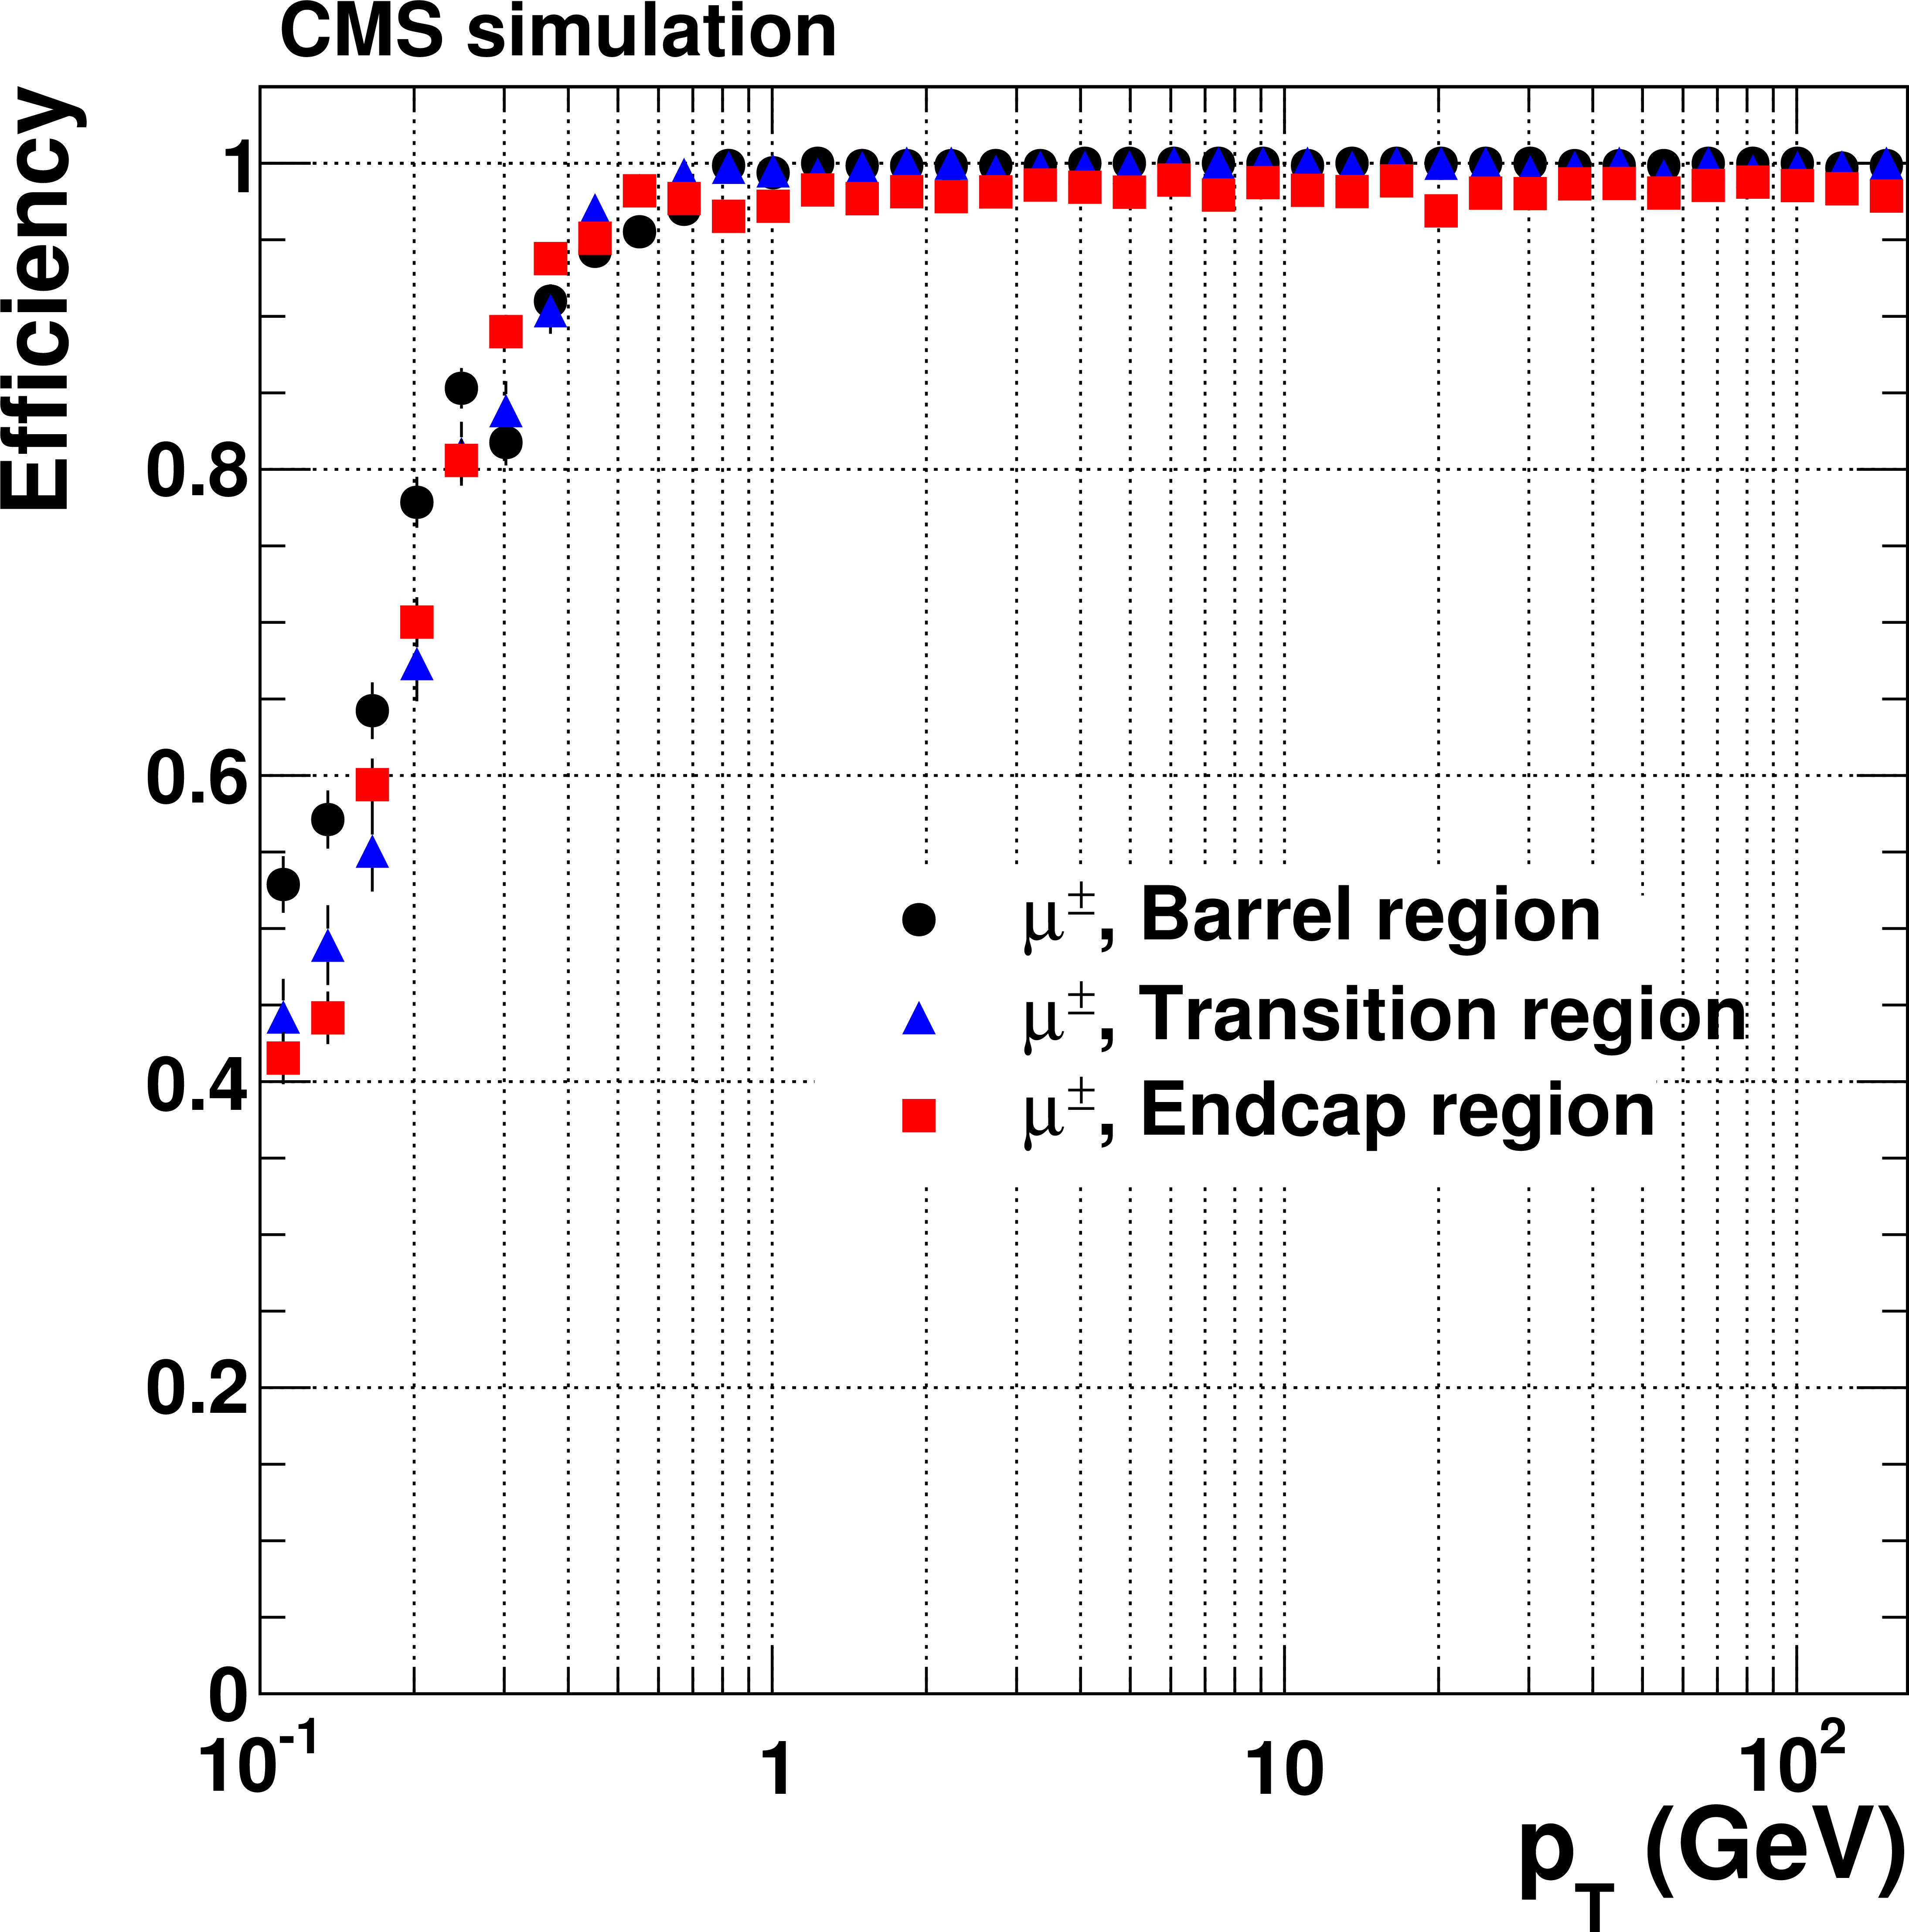
\includegraphics[width=0.35\textwidth]{figuras/Chapter3/TrackEff_Muon_pt.png}
    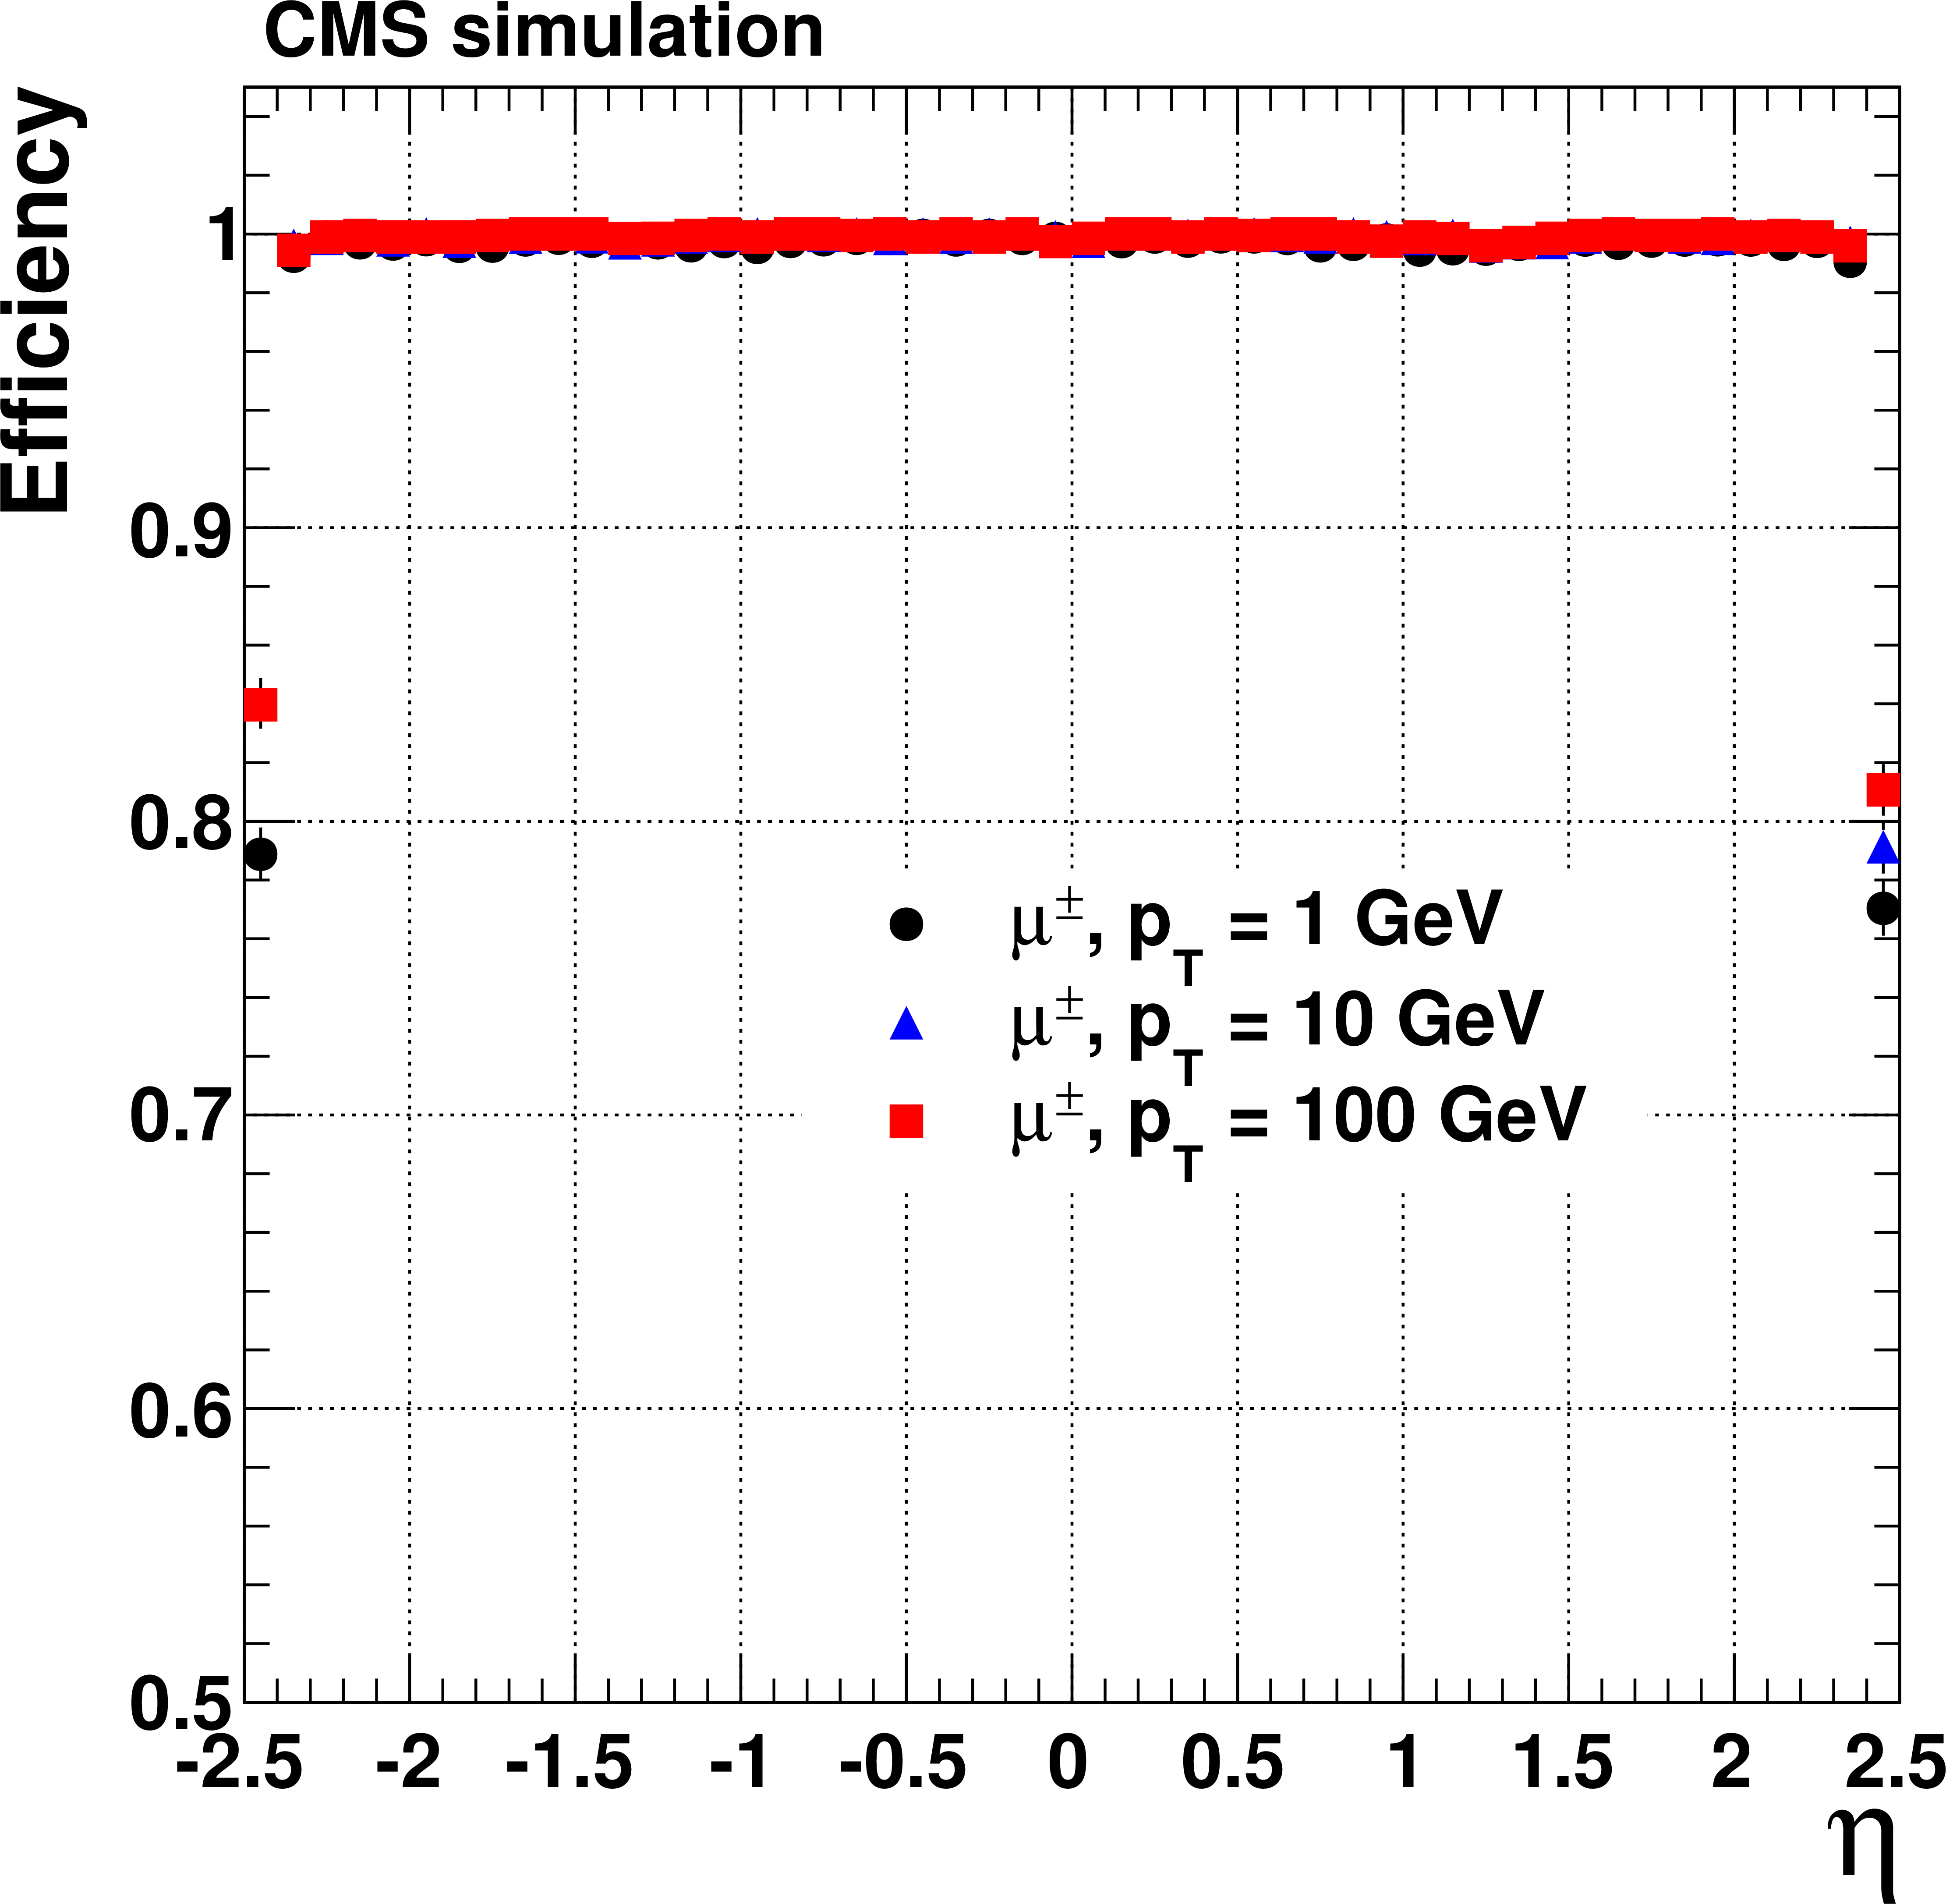
\includegraphics[width=0.35\textwidth]{figuras/Chapter3/TrackEff_Muon_eta.png}
    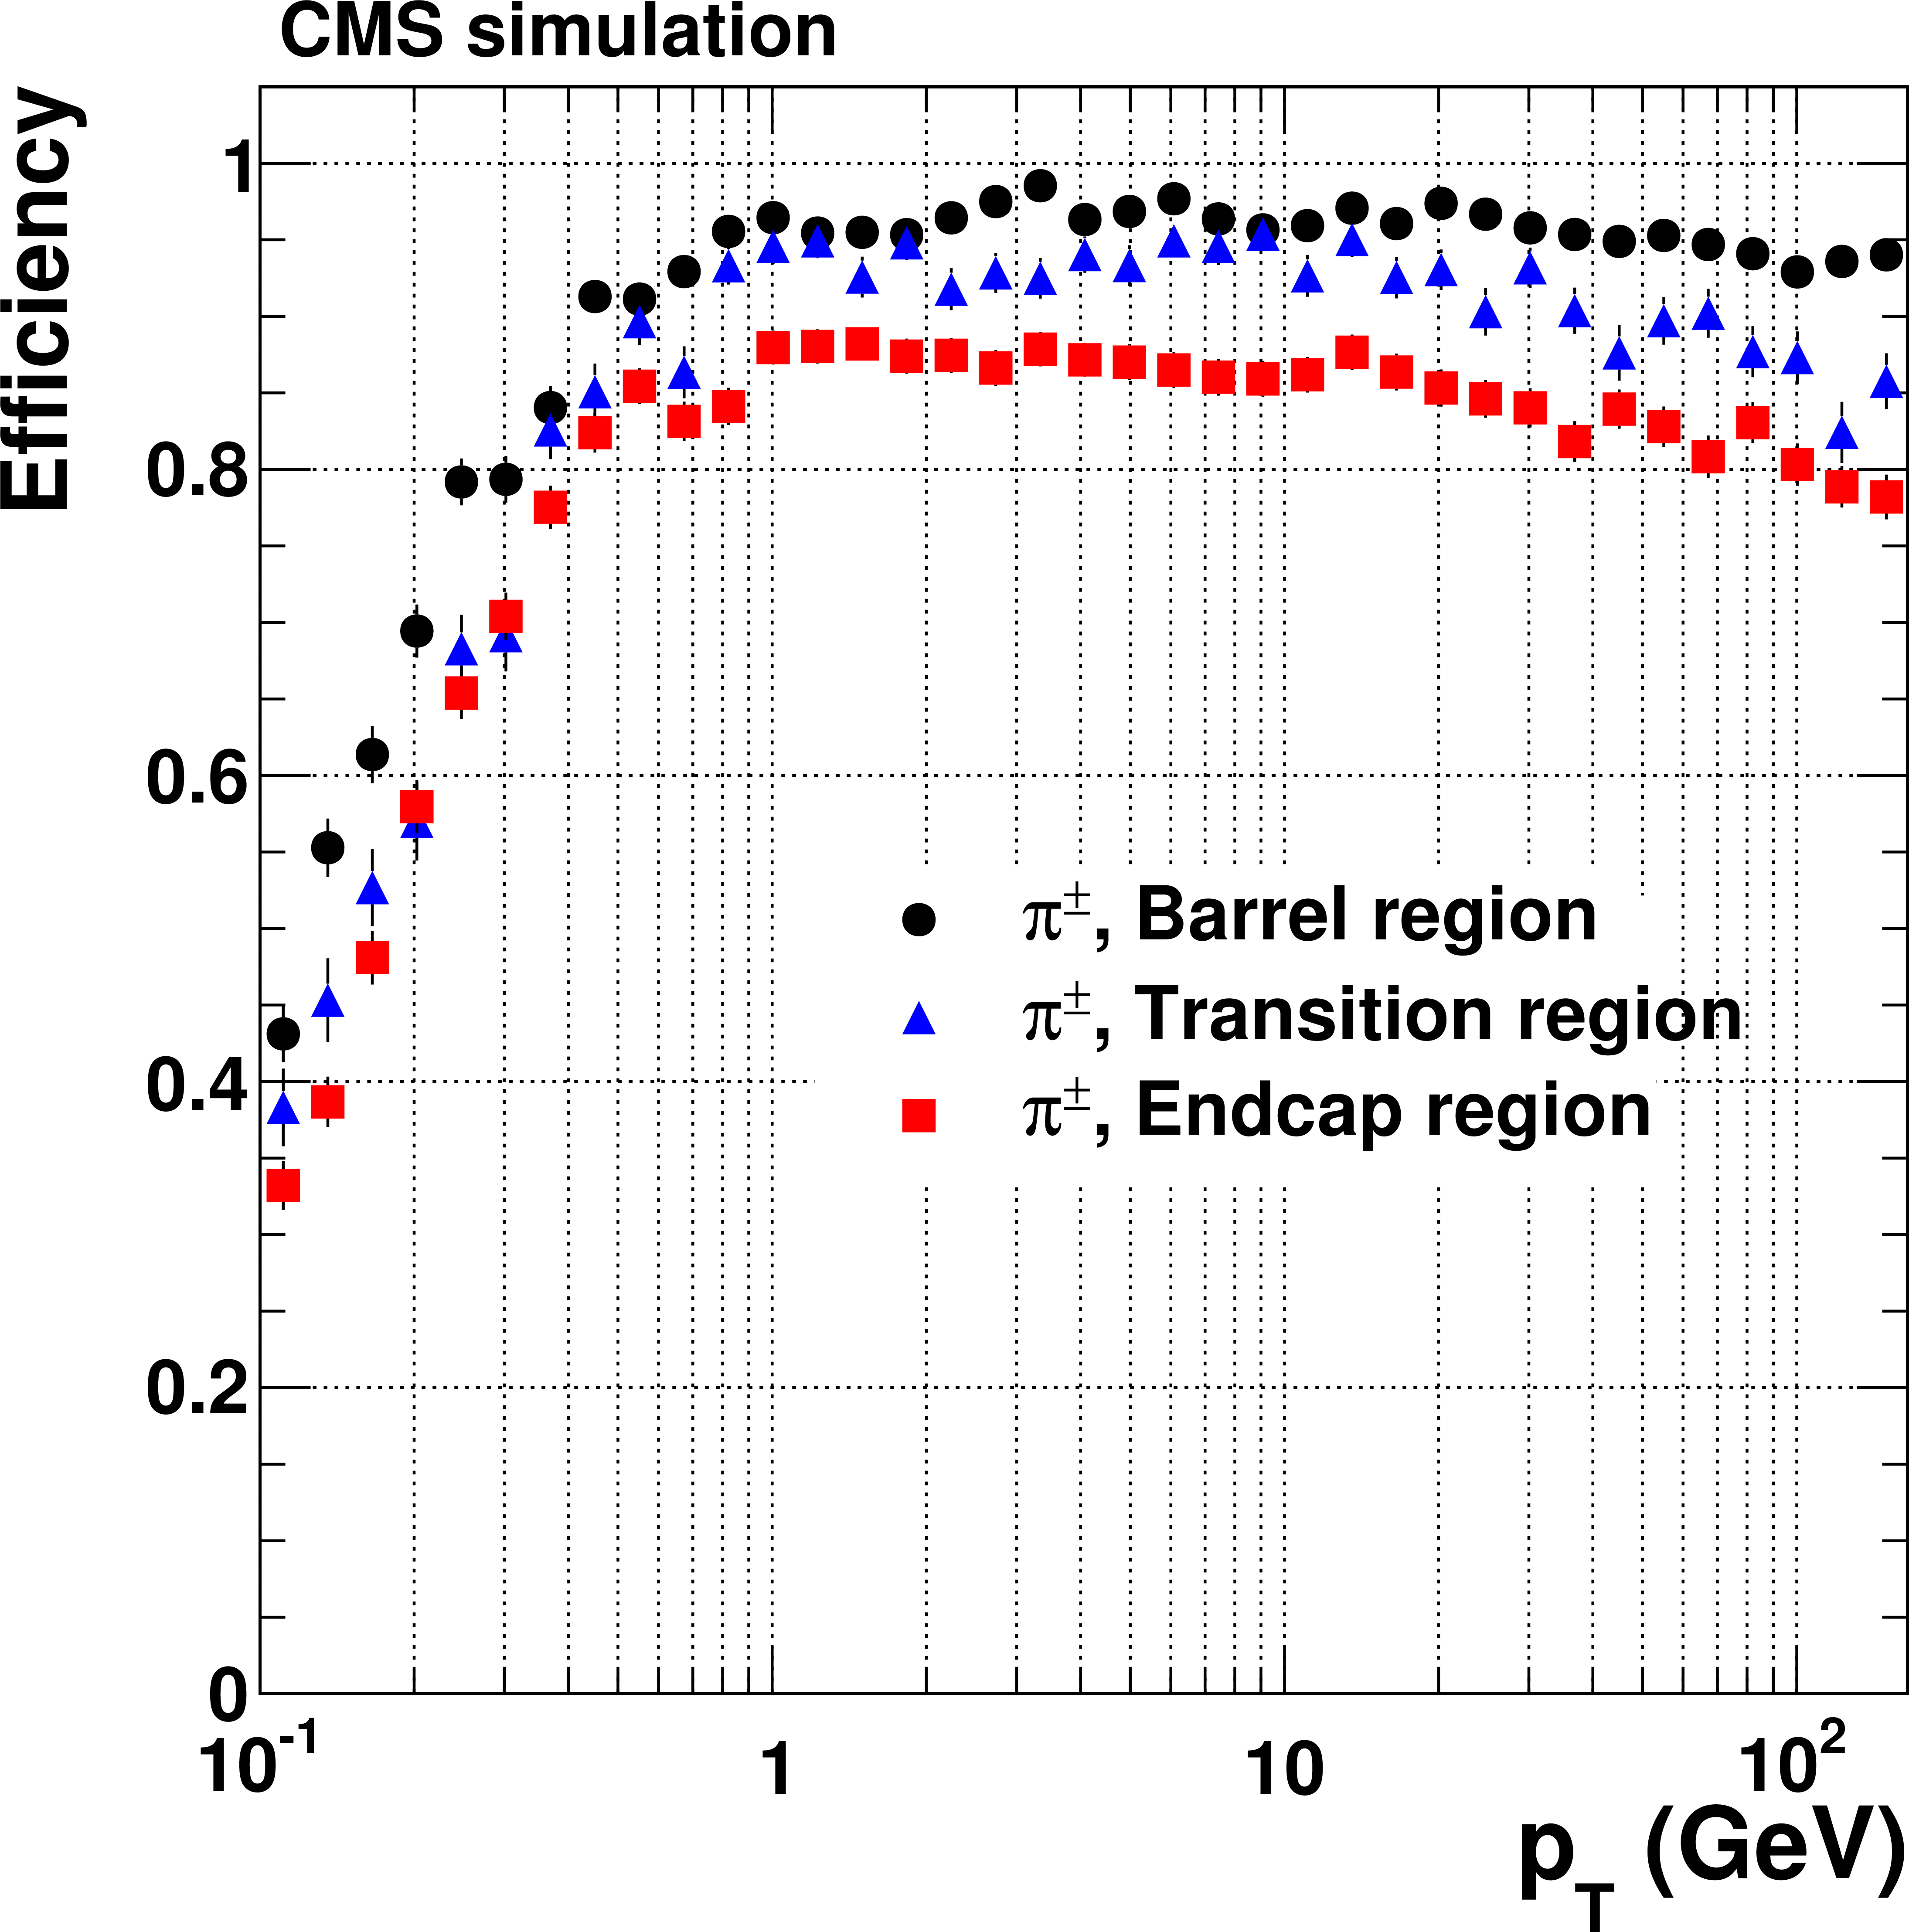
\includegraphics[width=0.35\textwidth]{figuras/Chapter3/TrackEff_Pion_pt.png}
    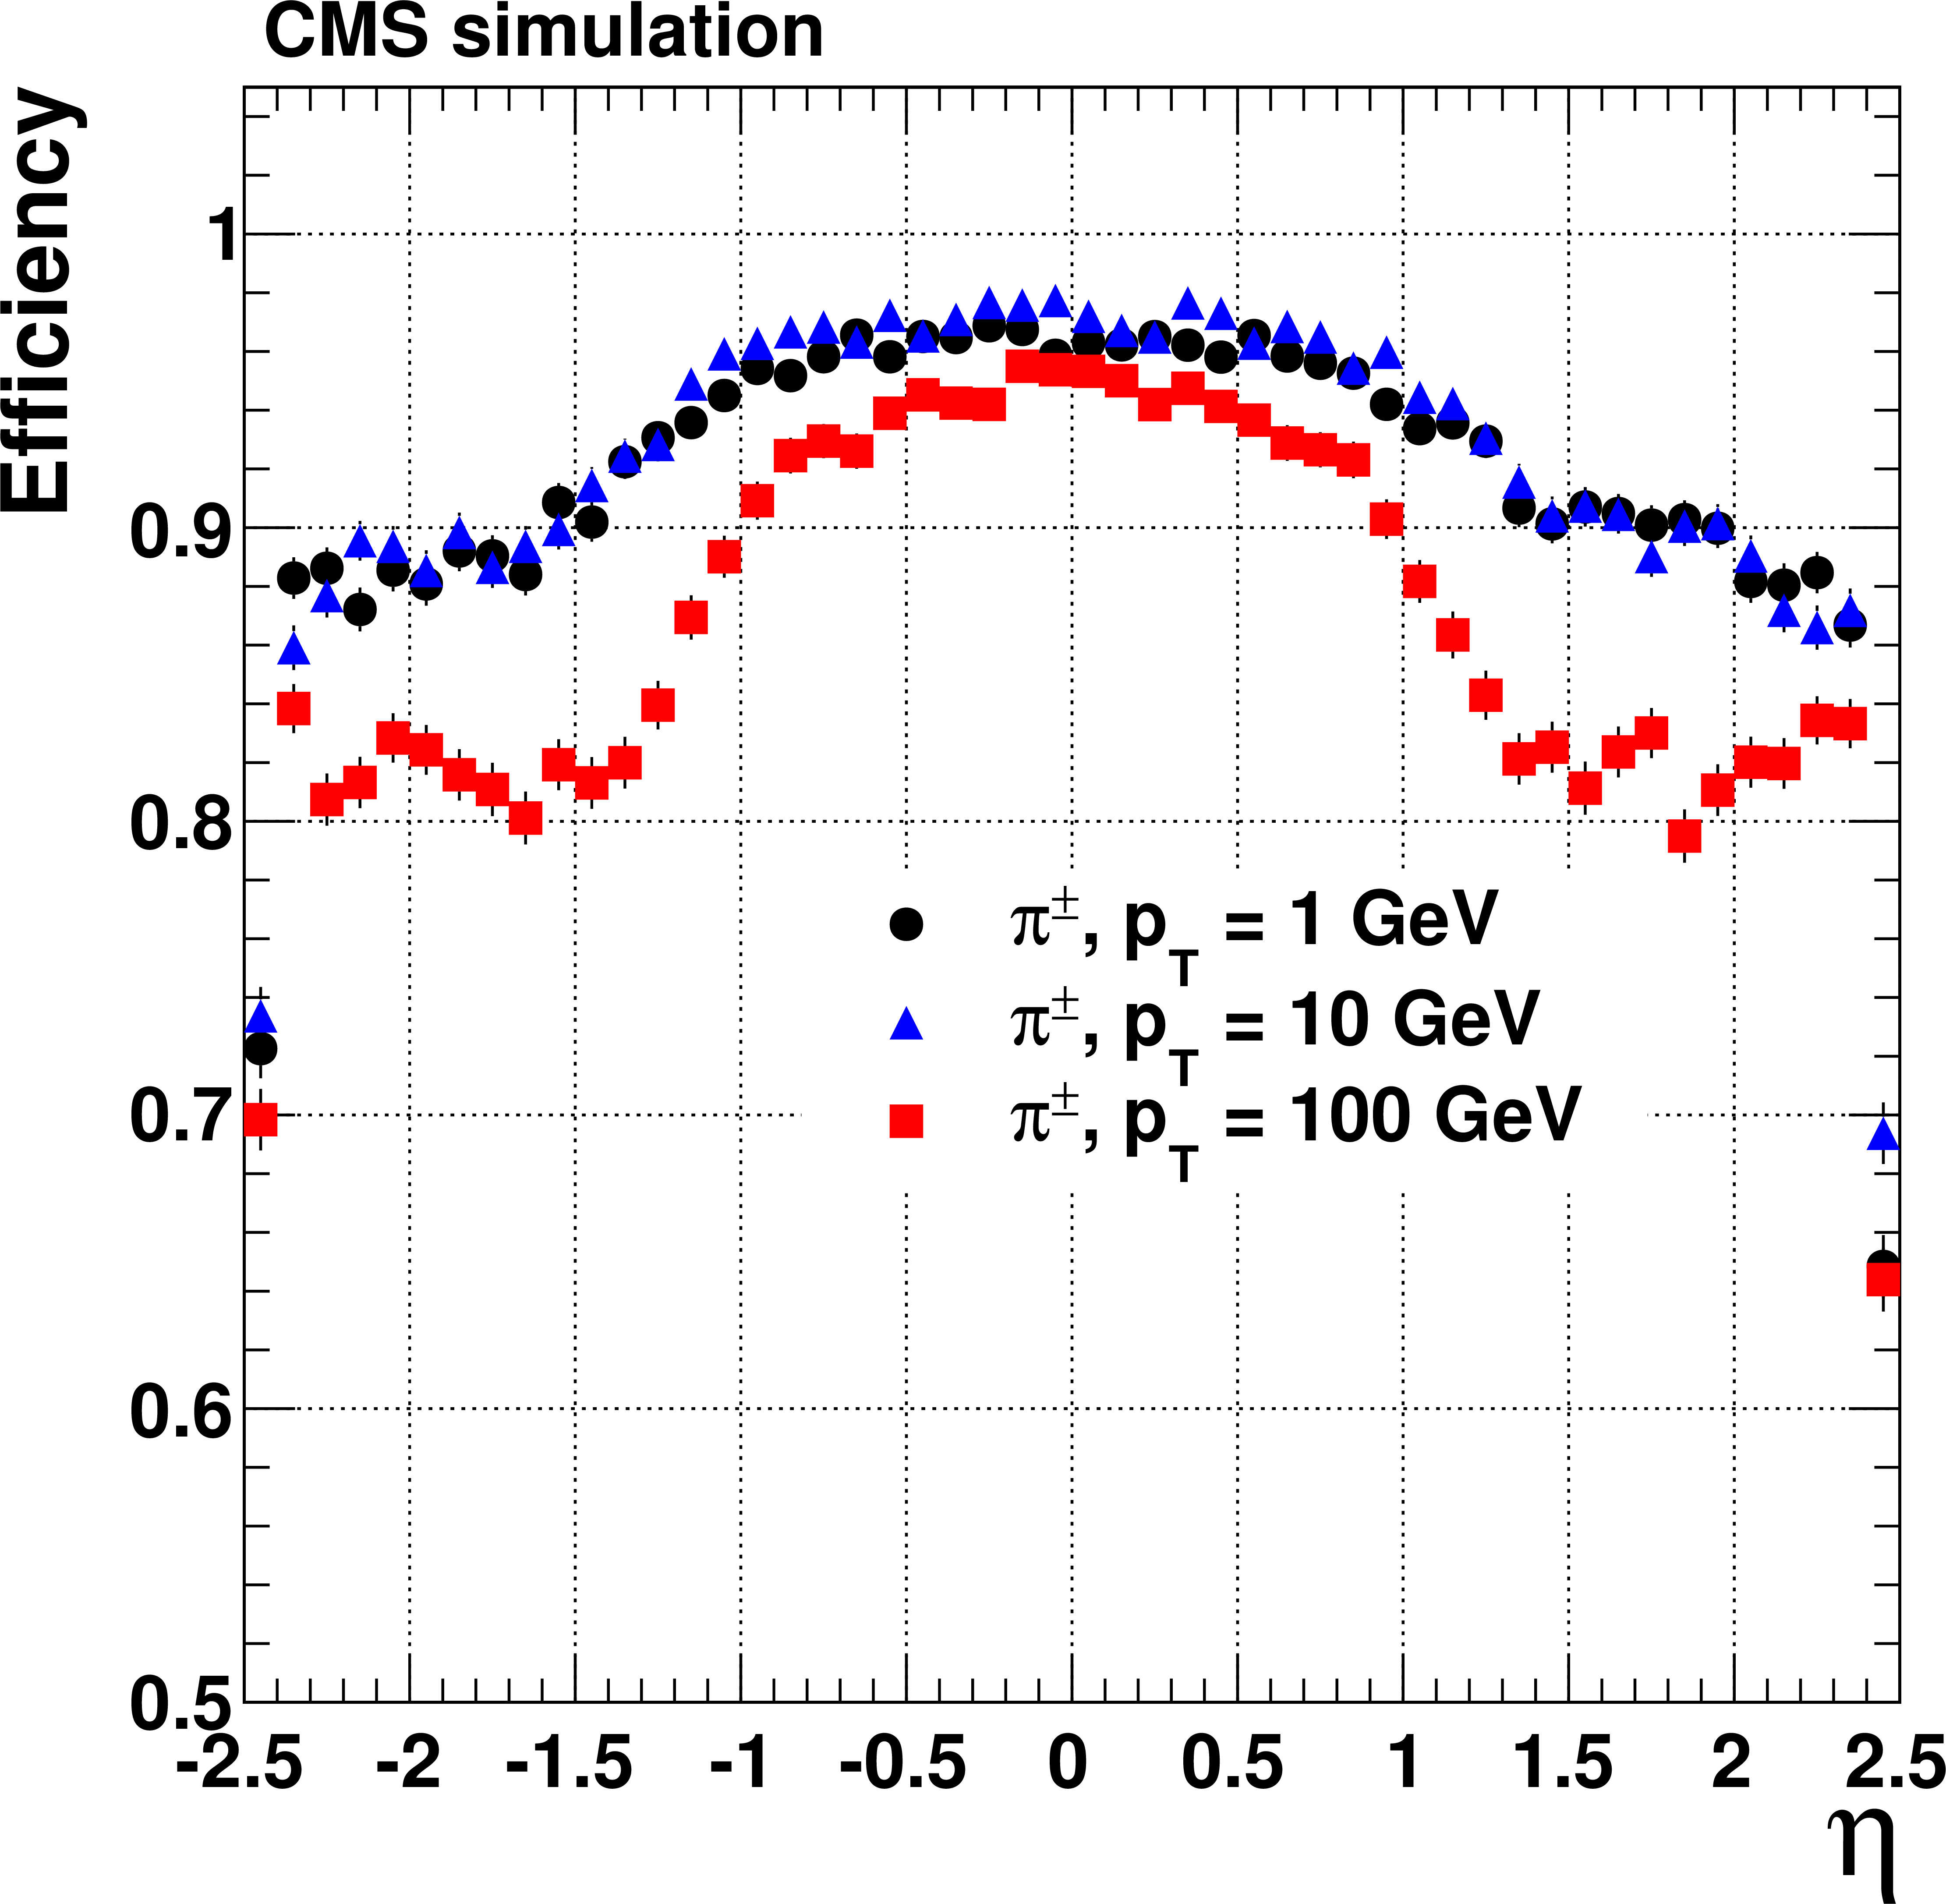
\includegraphics[width=0.35\textwidth]{figuras/Chapter3/TrackEff_Pion_eta.png}
    \caption{Efficiency of reconstructed tracks as a function of the \pt~(left) and the $\eta$ (right) for 
    muons (top) and charged pions (bottom). The efficiencies were obtained using data from pp collisions 
    with a \centermassenergy~of 7 \TeV, which corresponds to the 2011 data taking period. For simulated data 
    an average of 8 pileup events was used, which is roughly the amount delivered by the LHC in 2011. Figure taken from \cite{TrackAndVertexReconstruction}}.
    \label{fig:Track_Efficiencies}
  \end{center}
\end{figure}

\textbf{Vertex Reconstruction}\\

\noindent Vertex reconstruction is performed with the purpose to measure the position and the uncertainty
of all the vertices produced in the pp collision. It is performed in three stages: first, the 
algorithm selects the tracks that might come from the interaction region, according to 
their impact parameter, their number of the reconstructed hits associated
to the tracks (at least 2 hits in the pixel detector and at least 5 hits in the whole Tracker System) 
and the $\chi^{2}$ of their trajectory ($\leq $ 20). In the second step, the tracks
that might be produced from the same vertex are grouped into clusters; the track clustering 
is performed using the \textit{deterministic annealing} (DA) algorithm \cite{DAnnealing}, which 
identifies all the interaction points in a pp collision (even the inelastic collisions). Finally, 
the clusters of tracks associated to the same interaction point are fitted using an
\textit{adaptive vertex fitter} technique \cite{AdaptiveVertexFitting} with the purpose 
of estimating the vertex parameters, in particular its position. The primary vertex is identified
as the vertex with the higher sum of $\textrm{p}_{\textrm{T}}^{2}$ of the clusters of tracks.\\

\noindent The resolution of the primary vertex depends on the number of tracks associated to it. Figure \ref{fig:RecoVertex} 
shows the resolution of the x and z positions for the primary vertex reconstruction, using minimum-bias 
samples\footnote{Minimum-bias events pass a suit of triggers and minimum requirements on hit 
or track multiplicity.} and jet-enriched data samples \cite{TrackAndVertexReconstruction}. The resolution 
of the x position is less than 20 $\mu$m and of the z position is less than 25 $\mu$m, for the 
minimum-bias samples, while for jet-enriched samples are less than 10 $\mu$m and less than 
12 $\mu$m, respectively. Figure \ref{fig:RecoVertex} (c) shows
the efficiency of primary-vertex reconstruction as a function of the number of tracks. 

\begin{figure}[ht]
  \begin{center}
    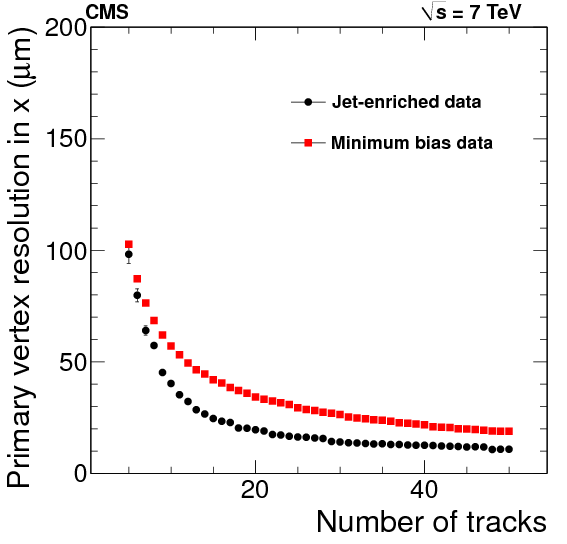
\includegraphics[width=0.3\textwidth]{figuras/Chapter3/RecoVertex_x_resolution.png}
    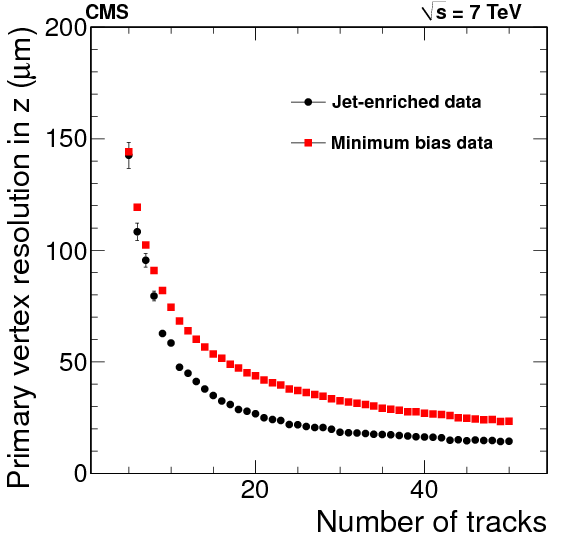
\includegraphics[width=0.3\textwidth]{figuras/Chapter3/RecoVertex_y_resolution.png}
    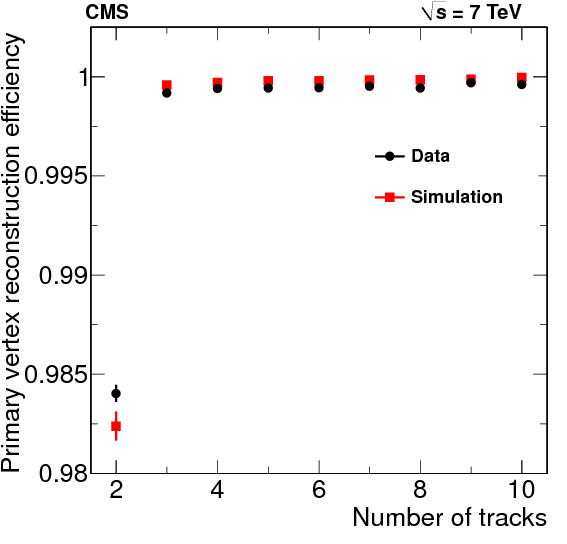
\includegraphics[width=0.3\textwidth]{figuras/Chapter3/Effciiency_vertex_resolution.png}
    \caption{Resolution of the x and z positions for primary vertex reconstruction, using a) minimum-bias samples and b) jet-enriched samples. 
    The resolution is improved using jet-enriched samples, since in these sample the \pt~mean is larger than minimum-bias samples.  
    For the primary vertex reconstruction efficiency shown in c), minimum-bias MC samples were used. These results were estimated 
    with pp collisions with a \centermassenergy~of 7 \TeV. Figures were taken from \cite{TrackAndVertexReconstruction}.}
    \label{fig:RecoVertex}
  \end{center}
\end{figure}


\subsection{Clustering}
\label{subsec:Clustering}

\noindent Other important PF elements, besides of the reconstructed tracks, are the calorimetric clusters. This
clustering is used for several purposes: to identify the 
energy deposits of photons and hadrons, allowing to discriminate neutral 
hadrons from charged hadrons; to provide additional information in order to 
determine the track parameters of the charged hadrons that were not measured 
accurately in the track reconstruction, for example, charged hadrons that pass outside 
of the tracker acceptance, or charged hadrons with high \pt; to reconstruction
of electrons along with their associated Bremsstrahlung radiation. \\

\noindent The clustering is performed for each part of the CMS calorimeter system: ECAL, HCAL, HF and PS. The 
clustering algorithm proceeds from the ``cluster seeds'' identified at local level. These seeds are selected from 
individual calorimeter cells whose energy deposits surpass a well defined threshold. Once a cluster seed is selected,
the algorithm searches for energy deposits in the  boundary cells. The algorithm adds to the cluster surrounding cells 
that have a maximum energy higher than two standard deviations from the electronic noise: 80 \MeV~for the ECAL Barrel,
300 \MeV~for the ECAL Endcaps and 800 \MeV~for the HCAL \cite{PFAlgorithm}. These combined cells are 
known as ``topological clusters''. The PF clusters are constructed from the topological 
clusters, avoiding any overlapping between them. 

\subsection{Link algorithm}
\label{subsec:Linkalgorithm}

\noindent As mentioned earlier, a particle is expected to produce signatures in different sub-detectors, giving rise to one or more 
PF elements: Tracker tracks, clusters and Muon tracks; for example, a charged hadron as the pion, would produce a 
track in the inner tracker along with energy deposits in both calorimeters. PF uses the \textit{link algorithm} to perform 
a topological combination of the PF elements coming form the different sub-detectors with the aim 
of fully reconstructing each particle in the event. \\

\noindent The link between a charged-particle track and a calorimeter cluster is performed as follows:

\begin{itemize}
 \item The track is extrapolated from the last hit reconstructed in the tracker to the two detection layers 
 in the case of PS, or the expected depth of a typical electron shower in the case of the ECAL, or
 one interaction length for a typical hadron shower in the case of the HCAL. 
 \item The track is linked to a calorimeter cluster if its extrapolated position is within the cluster boundaries. 
 \item The distance between the extrapolated track position and the cluster position, in the $\eta-\phi$ plane, defines the quality of the link. 
\end{itemize}

\noindent Similarly, the link of two calorimeter clusters (i.e. links between PS and ECAL clusters or links 
between ECAL and HCAL clusters) is performed when the extrapolated position from the more granular calorimeter (PS or ECAL) is within 
the boundaries of the less granular calorimeter (ECAL or HCAL). For example, the link between the ECAL and HCAL clusters
produced by one pion is established when the extrapolated position from the ECAL is within the HCAL cluster boundary. Finally, the 
link between a charged-particle track reconstructed in the Tracker System and a track reconstructed in the muon system is 
established by a global fit between the two tracks; its $\chi^{2}$ defines the quality of the link. This link is known as global
muon REF MUON RECO.

\subsection{PF Candidates}
\label{sec:PFCandidates}

\noindent Once the links are performed, the physics objects are identified by 
the Particle Flow algorithm according to their signatures in each sub-detector. The following
list shows the physics objects reconstructed individually:
\begin{itemize}
 \item \textbf{Muons} are reconstructed from the link between their signatures in the 
 Tracker System and the Muon Chambers. A PF muon is selected if the momentum measured 
 by the muon chambers is consistent with that measured by the Tracker within three standard deviations.
 \item \textbf{Electrons} are reconstructed from the link between a track and an ECAL cluster. The
 identification of electrons relies on their short tracks and their energy losses 
 due to  Bremsstrahlung. Their reconstruction is a complex task since the emitted Bremsstrahlung converts 
 into electron-positron pairs, whose tracks are bended due to the strong magnetic field; this leads to 
 energy deposits enlarged in the $\phi-$direction. Therefore, the PF electrons are built 
 from short tracks consistent with clusters enhanced in the $\phi-$direction.
 \item \textbf{Charged hadrons} are reconstructed using a link between a Tracker track and 
 clusters in the ECAL and the HCAL, for each hadron. However, there are 
 two scenarios in which the momentum of the track is not consistent with the energy measured 
 in the calorimeters: First, if the energy measured is less than the momentum 
 of the track, cleaning procedures are performed in order to discard spurious or mis-reconstructed 
 tracks, and then if there is consistency, a PF charged hadron is built; in cases 
 when there is still a difference between the energy measured and the momentum, a relaxed muon 
 search is performed. Second, if the energy measured is greater than
 the momentum of the track, the energy excess is attributed to the presence 
 of neutral particles: photons or neutral hadrons.
 \item \textbf{Neutral particles (photons and neutral hadrons)}, as mentioned above, are reconstructed 
 from the energy excess measured by the calorimeters compared with the momentum measured by the Tracker. Specifically, if
 this excess surpasses the total energy deposited in the ECAL, a PF photon is built with 
 the ECAL energy, while a PF neutral hadron is built using the remaining energy excess, otherwise
 only one PF photon is reconstructed. Additionally, PF photons and PF neutral hadrons can be 
 reconstructed from isolated ECAL clusters and isolated HCAL clusters, respectively.
\end{itemize}

\noindent Once all the visible particles are reconstructed individually, specific algorithms 
are used to reconstruct higher level objects such as jets, missing transverse energy and 
tau-leptons. The reconstruction of these objects which will describe in the following sections 
making emphasis in the case of the taus since they are crucial for this thesis. Besides, the jet, muon and 
electron reconstruction will also be described in detail since these physics objects can 
fake the tau signature.

\section{Muon Reconstruction and Identification}
\label{sec:Muon}

Muons are minimum ionizing particles with a long lifetime ($c\tau$ = 659 m); for 
this reason, they are capable to cross through the whole CMS detector 
without significant energy deposits and before their decay. In consequence, 
the muon identification is performed using the tracking information 
provided by the Tracker System (\textit{tracker tracks}) and by the Muon 
Chambers (\textit{standalone-muon tracks}). The tracker tracks were described
in section \ref{subsec:TrackReco}; the standalone-muon tracks are 
reconstructed through a linear fit of the hits detected
in the DT and CSC sub-systems, using the Kalman fitting 
technique \cite{KalmanAlgorithm}. Based on these two PF objects,
the muon reconstruction \cite{MuonID7TeV} is performed with 
three different approaches: 

\begin{itemize}
 \item \textbf{Global muon reconstruction (outside-in)}. Once a standalone-muon 
 track or hit is identified,  an extrapolation from the innermost muon stations to 
 the outer tracker surface is performed. If a tracker track is found and its 
 parameters (as its momentum) are consistent with those of the standalone-muon track, both trajectories
 are associated to the same muon. Then, all the hits coming from the Tracker System
 and the Muon Chambers are combined and fitted using the Kalman 
 filter technique \cite{KalmanAlgorithm}, which results in a reconstruction known as \textit{Global Muon}.
 This is particularly important for high-\pt~muons (\pt~$>$ 200 \GeV), since 
 the global fit can improve the momentum resolution compared with the one measured only with the 
 Tracker System information. 
 \item \textbf{Tracker muon reconstruction (inside-out)}. In this approach, the muon reconstruction 
 starts from the tracker tracks, with \pt~$>$ 0.5 \GeV, and 
 with a total momentum higher than 2.5 \GeV; these tracks are considered as 
 possible muon candidates and, consequently, they are extrapolated towards 
 the Muon Chambers. In order to match a tracker track with a standalone-muon 
 track, additional information is taken into account, such as the magnetic field,
 the energy losses and the multiple Coulomb scattering in the 
 detector material \cite{MuonID7TeV}. If at least one segment reconstructed in the Muon Chambers\footnote{
 A segment refers to the fit among the hits reconstructed in only one Muon Chamber (DT or CSC).} 
 is associated with the tracker track, the match is 
 classified as \textit{Tracker Muon}. The tracker muon reconstruction is especially
 important for low-\pt~muons (\pt~$>$ 5 \GeV~and \pt~$<$ 200 \GeV) due 
 to its high efficiency (since it requires only one muon-segment), 
 and to its high energy resolution in this kinematic range. 
 % reduces the hadron-to-muon misidentification rate.   
 \item \textbf{Standalone muon reconstruction}. When no tracker track is matched with the standalone muon track,
 the reconstruction results in a \textit{Standalone Muon}. They are not commonly used in CMS analyses since they 
 have the worst momentum resolution compared with the Global Muons and the Tracker Muons. Additionally, their 
 signature can come from cosmic-ray muons.
\end{itemize}

\noindent The high efficiency of the tracker tracks and the standalone tracks
allows to reconstruct 99$\%$ of the muons produced in the pp collisions within the geometrical 
acceptance \cite{MuonID7TeV}. A muon can be built as a Global Muon or as a Tracker Muon using either 
of both approaches; besides, in the case that one muon is reconstructed using both of 
them, the information is merged into one single muon candidate. Once the muon 
candidate is selected, several algorithms are applied in order to 
identify it from background processes that can fake the muon 
signature, such as charged hadrons. Charged hadrons can cross the whole 
Calorimeter System and can reach the Muon Chambers, producing similar signatures tho those of a muon,
with the exception of the energy deposits in the calorimeters. Therefore, the energy-loss requirement 
 allows to discriminate muons from charged hadrons. There are three basic muon identification 
 algorithms: the soft muon selection, the tight muon selection, and the global 
 selection (a more detailed description of each algorithm can be found in 
 reference \cite{MuonID7TeV}). The PF algorithm uses these identification
 requirements and, along with the energy deposits in the Calorimeter System, it selects 
 the so called PF Muon Candidates. \\

\noindent  The PF Muons are identified using three different selections known as ``isolation'', ``pf-tight''
 and ``pf-loose'' \cite{PFMuonAndElectron}. The isolation selection looks for muons with low neighboring activity, defining 
 a cone of \DR~$=$ 0.4 around the muon trajectory. If the sum of the \pt~of the tracks and the 
 transverse energy deposited in the calorimeters, within the cone, is less than 15$\%$ of the muon \pt, an ``isolated'' muon 
 is selected. The main goal of pf-tight and pf-loose selections is the identification of muons within jets. The 
 pf-tight selection requires a minimum amount of hits in the Muon Chambers and searches for compatibility between 
 the momentum measured and the energy deposited in the calorimeters. When the momentum is 
 significantly higher than the energy deposits, which is compatible with the muon signature, 
 but not with the charged hadron signature, the pf-loose selection is applied. In consequence, the last selection 
 discriminates between muons and charged hadrons in a jet, relaxing the number of hits required 
 and looking for matches between the tracker track and the standalone-muon track. \\
  
 %The performance of the muon identification and the relative isolation for 
 %the operating points used this analysis is shown in Figure \ref{fig:MuonPerformance}.
 
 %\begin{figure}[ht]
 % \begin{center}
 %   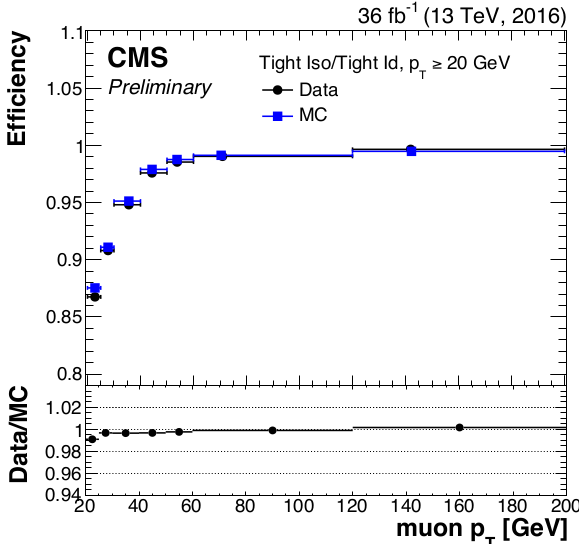
\includegraphics[width=0.4\textwidth]{figuras/Chapter3/MuonIsoPT.png}
 %   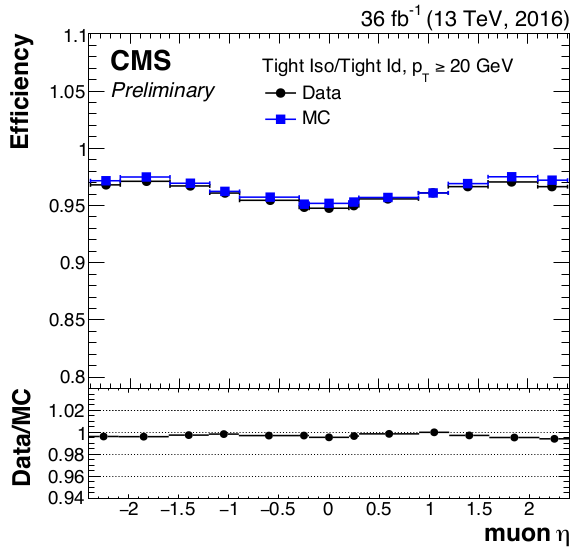
\includegraphics[width=0.4\textwidth]{figuras/Chapter3/MuonIsoEta.png}
 %   \caption{ \cite{MuonPerformance}.}
 %   \label{fig:MuonPerformance}
 % \end{center}
%\end{figure}

\section{Electron Reconstruction and Identification}
\label{sec:Electron}

\noindent The electron reconstruction relies on the association of an ECAL cluster
and a track reconstructed in the Tracker System. This is challenging 
since electrons lose energy through Bremsstrahlung radiation
while crossing the Tracker material, therefore, their energy deposits are 
spread out in several ECAL crystals, mostly in the $\phi$-direction,
due to the bending of the electron tracks caused by the magnetic 
field (see Figure \ref{fig:ElectronScketch}). Because of its
interactions with the Tracker material, an electron can lose of the order of 33$\%$ of its 
energy crossing the central region of the Tracker System ($|\eta| \sim 0$) where 
the material budget is minimum, whereas 86$\%$ of its energy is 
lost by photon radiation if it passes through the Tracker at $|\eta| \sim 1.4$ \cite{ElectronID8TeV}. In 
consequence, the collection of the energy coming from Bremsstrahlung radiation is crucial for an accurate 
measurement of the initial energy of the electron. \\


\begin{figure}[ht]
  \begin{center}
    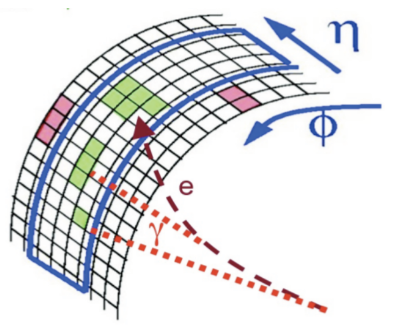
\includegraphics[width=0.4\textwidth]{figuras/Chapter3/ElectronCluster.png}
    \caption{Schematic view of energy deposited by an electron in the ECAL.}
    \label{fig:ElectronScketch}
  \end{center}
\end{figure}


\noindent There are two algorithms to measure the initial energy of the 
electron using the information provided by the ECAL: the ``hybrid'' algorithm for 
the barrel and the ``multi-5$\times$5'' algorithm for the endcaps. The hybrid algorithm
searches for several clusters consistent with energy deposits enlarged in the $\phi$-direction, as 
was mentioned above. It starts selecting the seed crystal\footnote{The seed crystal has 
the higher collected energy in a defined region.} and then, it looks 
progressively for crystals, in both $\phi$ directions, that exceed a threshold 
energy. These crystals are grouped, resulting in the so called \textit{supercluster} (SC). In the 
case of the ``multi-5$\times$5'' algorithm, since the endcap crystals are not arranged in 
a $\eta-\phi$ geometry, a crystal is selected based on the high energy deposit and an 
arrange of 5$\times$5 crystals centered on it are selected. The cluster reconstruction is complemented 
with the PF algorithm, adding the contiguous crystals to the seed, whose 
energy collected exceeds two standard deviations above the electronic noise
(230 \MeV~in the barrel and 600 \MeV~in the endcaps). \\

%it selects the crystal seed and defines the SC as an arrange of 5$\times$5 crystals centered on it. 


\noindent The electron track reconstruction is also challenging due to the significant energy losses by 
Bremsstrahlung in each Tracker layer, which can cause a considerable variation in the 
curvature of its trajectory; this results in a degradation of the performance of the track reconstruction.
For this reason, the Kalman Fitter (KF) algorithm used for all charged particles is not appropriated to reconstruct
the electron track and instead a Gaussian Sum Filter (GSF) \cite{ElectronGSF} algorithm has been developed with 
this purpose. Since the pattern recognition procedure can be very time consuming, the algorithm
starts preselecting tracks seeds. There are two algorithms used for the electron track reconstruction:
the first one is called \textit{seeding} and the other one is called \textit{tracking}. The seeding
algorithm performs an extrapolation from the SC to the Tracker System in order to 
select hits compatible with, either positive or negative charge hypotheses; then, the selected hits  are 
used as input for a preliminary track reconstruction, which is performed with the
the general algorithm for charged particles, extrapolating the track towards the ECAL 
and matching it to a SC. The tracking algorithm looks for additional
hits consistent with the electron track, discarding any ambiguity; it uses the Kalman Fitter method 
in each successive layer, including the energy loss by the electron. Once the hits collection is set, 
without ambiguities, a GSF fit is performed to estimate the track parameters. As a result, 
the algorithm provides an electron track that can be extrapolated to the ECAL, whose
energy loss by Bremsstrahlung can be estimated as: $f_{brem} = (p_{in}-p_{out})/p_{in}$, where
$p_{in}$ is the momentum measured in the inner-most layer of the Tracker system, while $p_{out}$
is the momentum at the ECAL surface, estimated from the extrapolation.  This variable is useful
for the electron identification.\\

\noindent Once the PF cluster candidates and the GSF tracks are selected, the algorithm builds 
the PF electron candidates, looking for geometrical matches between them. The matching is set 
when $|\Delta \eta| = | \eta_{SC} -\eta_{in}^{extra} | <$ 0.02, where $\eta_{SC}$ is the
$\eta$ position of the SC energy and $\eta_{in}^{extra}$ is the $\eta$ position of the 
extrapolated track from the inner track layer to the ECAL surface. Similarly, for the $\phi$-direction,
 $|\Delta \phi| = | \phi_{SC} -\phi_{in}^{extra} | <$ 0.15 is required.\\
 
\noindent CMS uses several algorithms to identify isolated electrons (signal) and to distinguish
them from processes that can fake their signature, such as photon conversions, jets 
misidentified as electrons,  hadronic taus misidentified as electrons, or electrons 
produced from semileptonic decays of b and c quarks. In this analysis, a MVA-based
algorithm is used for electron identification, exploiting  the information of the
track-cluster matches, the SC geometrical structure, the $f_{brem}$ fraction, among others. 
Different working points are defined according to the desired reconstruction efficiency for 
each analysis (see Table \ref{eIDtable}). In order to reduce the electron-to-tau 
misidentification rate, the 90$\%$ efficiency working point of the MVA 
electron ID is selected for this analysis.\\

\begin{table}[ht]                                                                                                                              
\begin{center}
  \begin{tabular}{| l | c | c | }
 \hline\hline
       Category                             & MVA$_{\textrm{min cut}}$ (80\% signal eff)    & MVA$_{\textrm{min cut}}$ (90\% signal eff)  \\ \hline 
       Barrel ($\eta < 0.8$) $p_{T}>10$     & 0.941                                         & 0.837                     \\
       Barrel ($\eta > 0.8$) $p_{T}>10$     & 0.899                                         & 0.715                     \\
       Endcap $p_{T}>10$                    & 0.758                                         & 0.357                     \\
 \hline
 \hline
 \end{tabular}
 \caption{Electron ID Selections.\label{eIDtable}}
\end{center}
\end{table}

\noindent An additional background reduction is obtained through an isolation requirement. Jets or
electrons coming from semileptonic decays of b or c quarks can fake the signature 
of electrons coming from the primary interaction. Since both cases have a significant
energy deposits around their tracks, an isolation requirement will reduce considerably 
these background contaminations. The relative isolation is defined as:

\begin{equation}
\text{Iso}_{\text{PF}}~= \frac{ \Sigma \text{p}_\text{T}^{\text{charged had}} + \text{max}[0, \Sigma \text{p}_\text{T}^{\text{neutral had}}
+ \Sigma \text{p}_\text{T}^{\gamma} - 0.5 \times \Sigma \text{p}_\text{T}^{\text{charged hadrons from PU}}]}{\text{p}_\text{T}^{\text{electron}}} \;,
\end{equation}

\noindent where the sums run over the charged hadron candidates, neutral hadrons and photons, within
a $\Delta R$ cone around the electron direction. The charged hadron candidates are required to be
originated from the primary vertex \cite{ElectronID8TeV} and a correction due to PU contributions is included 
($\text{p}_\text{T}^{\text{charged hadrons from PU}}$). In this analysis, the isolation requirement used is
$\Delta R <$ 0.4.


\section{Jet Reconstruction}
\label{sec:Jet}

\noindent Quarks and gluons produced by the pp collisions, at parton level, have a 
well defined color charge and, due to the confinement of the strong 
interaction, they can not exist as free particles; instead, they 
will follow a process of fragmentation and combination with quarks and gluons from the vacuum to form 
colorless bound states called hadrons; this process is known as hadronization. The hadronization will 
give rise to showers of particles, which propagate in a similar direction forming a cone; this set 
of particles is known as a jet (see Figure \ref{fig:JetScketch}). The aim of a jet reconstruction 
algorithm is to determinate the energy and the direction of the initial parton. The PF technique 
reconstructs all the particles individually, from the information collected by the CMS sub-detectors,
and then cluster them into the jet, determining the compositeness and, 
when possible, its the initial parton. \\

\begin{figure}[ht]
  \begin{center}
    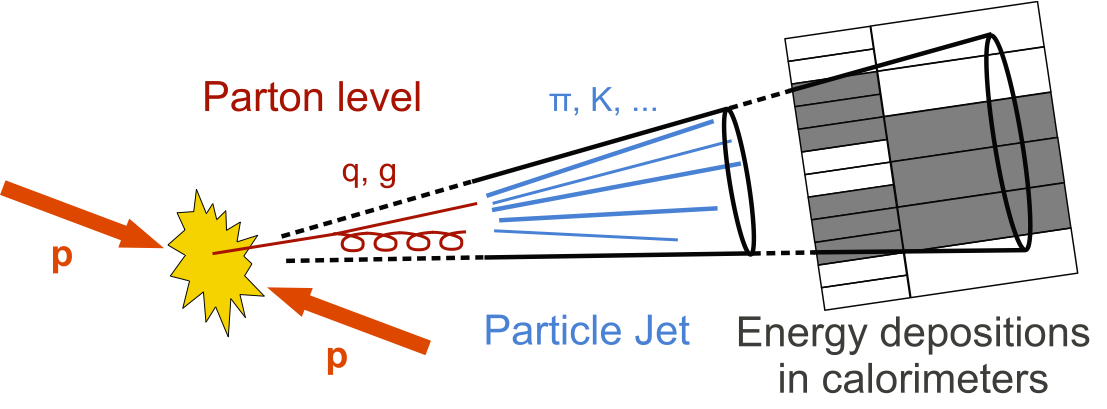
\includegraphics[width=0.6\textwidth]{figuras/Chapter3/JetSketch.png}
    \caption{Schematic diagram of the evolution and detection of a jet.}
    \label{fig:JetScketch}
  \end{center}
\end{figure}

\noindent The signature of the jet in each layer is expected to be located roughly 
into an area of $\pi R^{2}$, where $R$ is used as an input parameter of 
the reconstruction algorithms. The parameter $R$, and 
consequently the jet area in a given layer, determine the sensitivity of the algorithm to discriminate between 
jets and soft radiation processes. If the $R$ parameter is too large, not 
only all possible particles coming from the hadronization are included in the reconstruction,
but also those coming from the underlying event (UE) or pileup collisions (PU) might 
be included; this will lead to an overestimation of the jet energy. Additionally, the 
algorithm must consider other important circumstances that degrade
the jet-reconstruction efficiency, such as the \textit{infrared} and the \textit{collinear} 
scenarios. The infrared processes refer to soft QCD radiation that might be wrongly included in the jet 
reconstruction, altering the jet components. The collinear processes refer to parton 
splitting into collinear components, leading to the reconstruction of a different 
number of jets. The algorithms that avoid including these processes are known 
as infrared- and collinear-safe algorithms (ICR).\\

\noindent There are two different types of algorithms that have been used for jet reconstruction: the cone algorithms (SISCone)
and the sequential clustering algorithms (kT, Cambridge-Aachen, anti-kT). The main difference between them 
is the way how the particles which belong to a jet are clustered. The cone algorithms consider that the particles 
in a jet are spread out in a rigid conical region, which results in a fixed definition of the jet area, while the
sequential algorithms assume fluctuations on the jet area, where the boundaries are 
defined with a fixed maximum radius. The main features of these algorithms are:

\begin{itemize}
 \item \textbf{SISCone algorithm}: checks all the particles in the event in order to 
 identify stable combinations that are coherent with a jet. This algorithm explores randomly the $\eta-\phi$ plane
 using a circle, with a well defined area, until a particle matches with the circumference; then, the circumference
 is pivoted until a second particle comes in contact with it. The matches define the stable cones. The particles
 associated to an stable cone are removed from the list of particles of the event and the procedure is performed again 
 until no more stable cones are found. Finally, the stable cones are split or merged, according to an overlap parameter, in order to 
 reconstruct the jets \cite{ICRJet}. 
 \vspace{0.3cm}
 
 \item \textbf{kT-algorithm}: estimates the following distance variables for all pair of particles ($i,j$):
\begin{equation} \label{eq:kt}  
 \begin{aligned}
  d_{ij} &= min(p_{Ti}^{2},p_{Tj}^{2})\Delta R_{ij}^{2}/R^{2} \;,\\
  d_{iB} &= p_{Ti}^{2} \;,
  \end{aligned}
  \end{equation}

\noindent where $\Delta R_{ij}^{2}=\Delta(\eta_{i},\eta_{j})^{2}+\Delta(\phi_{i},\phi_{j})^{2}$ is the distance 
in the $\eta-\phi$ plane between the particles $i$ and $j$, $R$ is the radius parameter that 
defines the size of the jet, and $d_{iB}$ is the distance between the beam axis and the particle $i$. Then, the algorithm
proceeds by finding the minimum distances $d_{ij}$ and $d_{iB}$; if $d_{ij}$ is a minimum, the pair 
of particles $i,j$ are recombined adding their four-momenta; if $d_{iB}$ is a minimum, the algorithm
identify the particle $i$ as a jet. The distances are recalculated iteratively until all particles are  %%%OJO 
part of the jet \cite{ktalgorithm, ICRJet}. 
 \vspace{0.3cm}
\item \textbf{Cambridge-Aachen algorithm}: proceed similar to the kT algorithm, but defining 
 the variable distances:

 \begin{equation}   \label{eq:Cambridge-Aachen}
 \begin{aligned}
  d_{ij} &= \Delta R_{ij}^{2}/R \;,\\
  d_{iB} &= 1 \;.
  \end{aligned}
  \end{equation}
\noindent Since $d_{ij}$ is independent of the momentum, the jet size will not 
be clearly defined and UE and PU processes will be included in the jet reconstruction. In spite of 
that disadvantage, this algorithm is commonly used since it allows to determine the 
jet compositeness \cite{Cambrigdealgorithm}.
 \vspace{0.3cm}
 \item \textbf{anti-kT algorithm}: defines the following distance variables for all particles pairs ($i,j$):

 \begin{equation}   \label{eq:antikt}
 \begin{aligned}
  d_{ij} &= min\left(\frac{1}{p_{Ti}^{2}},\frac{1}{p_{Tj}^{2}}\right)\Delta R_{ij}^{2}/R^{2} \;,\\
  d_{iB} &= \frac{1}{p_{Ti}^{2}} \;. \\
  \end{aligned}
  \end{equation}
\noindent The anti-kT algorithm follows the same procedure as the kT algorithm. It calculates 
iteratively the variables $d_{ij}$ and $d_{iB}$, and searches 
for the minimum of the set $\{d_{ij},d_{iB}\}$. If $d_{ij}$ is a minimum, the 
particles $i$ and $j$ are merged by the algorithm and they are treated as one 
particle; the iterative procedure continues until the $d_{iB}$ minimum is found. If $d_{iB}$ is a
minimum distance, the particle $i$ is identified as a jet, which means that
all the particles merged by the algorithm associated with that particle $i$ 
are the constituents of the jet. Since the anti-kT $d_{ij}$  variable is 
dominated by high $p_{\textrm{T}}$ particles, the algorithm will first merge them, resulting 
in an accurate jet area estimation \cite{AntiKTAlgorithm}. %%%OJO
\end{itemize}

\noindent The anti-kT algorithm is used in most of the CMS and ATLAS analyses. The advantage of  
this algorithm is related with the jet area since, as mentioned above, it calculates first 
the distance for the high \pt~particles and then recalculates 
this distance, including low \pt~particles; this results in a slight 
fluctuation in the jet area, which is important for removing any 
contributions from UE and PU processes. Figure \ref{fig:JetsAlgos} presents an example of 
the jet area profile using the algorithms described above, showing the 
advantage of the anti-kT algorithm. \\

\begin{figure}[ht]
  \begin{center}
    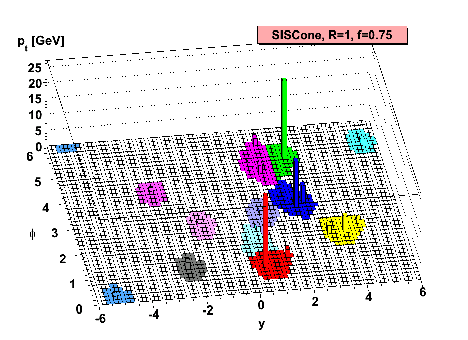
\includegraphics[width=0.43\textwidth]{figuras/Chapter3/herwig-parton-level-ev-siscone-R1-0-f0-75-ghosted4root.png}
    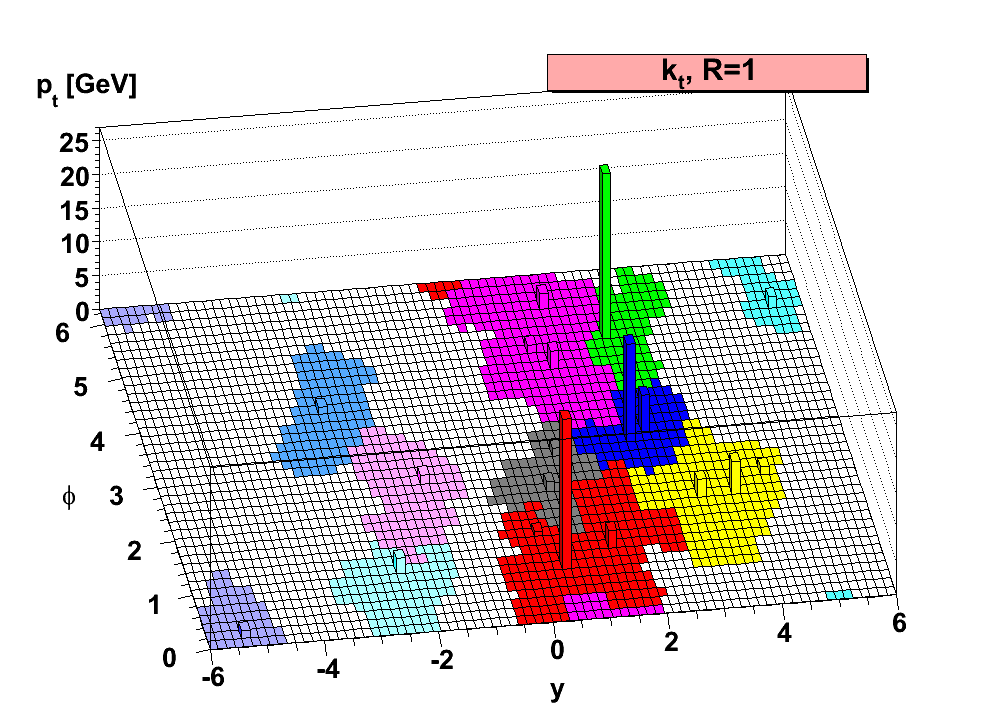
\includegraphics[width=0.43\textwidth]{figuras/Chapter3/herwig-parton-level-ev-kt-R1-0-ghosted4root.png}
    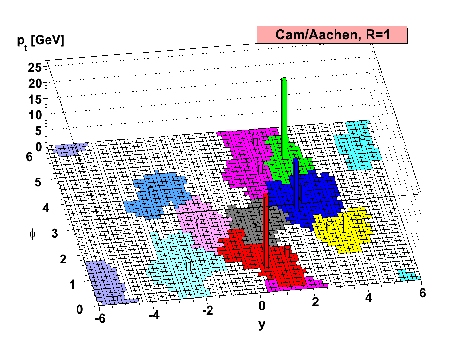
\includegraphics[width=0.43\textwidth]{figuras/Chapter3/herwig-parton-level-ev-cam-R1-0-ghosted4root.png}
    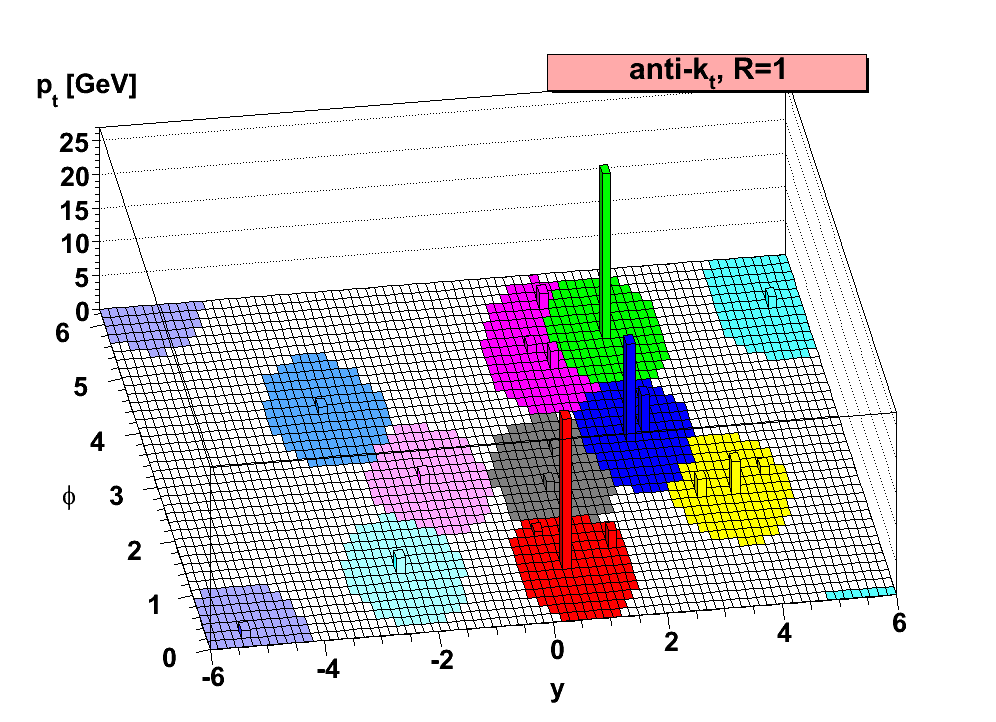
\includegraphics[width=0.43\textwidth]{figuras/Chapter3/herwig-parton-level-ev-antikt-R1-0-ghosted4root.png}
    \caption{Jets reconstruction using the algorithms: SISCone (left-top), kT (right-top), Cambridge-Aachen 
    (left-bottom) and anti-kT (right-bottom). The jet reconstruction was performed with MC samples using the same $R$
    for all the algorithms. The SISCone algorithm reconstructs jets in smaller well defined area 
   but it identifies two different jets instead of the one (see jet in color gray); the kT algorithm results an 
   irregular jet area since it starts the reconstruction using the low \pt~particles; the Cambridge-Aachen 
   algorithm also shows an irregular jet area, since the distances between particles are 
   independent of their momenta; and the anti-kT algorithm shows a well defined area, reconstructing 
   the proper number of jets \cite{Cambrigdealgorithm}.} \label{fig:JetsAlgos}
  \end{center}
\end{figure}
 
\noindent The CMS jet reconstruction is performed with the anti-kT algorithm, setting 
the distance parameter $R$ in the $\eta-\phi$ plane to $0.4$. The four-momentum of the 
reconstructed jet corresponds to the sum of the four-momenta of all 
the PF objects associated to it. However, 
due to detector response and experimental effects, the 
reconstructed PF jet four-momentum does not correspond to the one
at parton or hadron level, in consequence, corrections must be applied
to the jet energy. These corrections are known as 
\textit{Jet Energy corrections} (JEC) \cite{JECpileup,JESandJER}. Different levels of JEC 
(see Figure \ref{fig:JEC_levels}) are applied in a fixed sequence: \\

\begin{figure}[ht]%[!Hhtbp]
  \begin{center}
    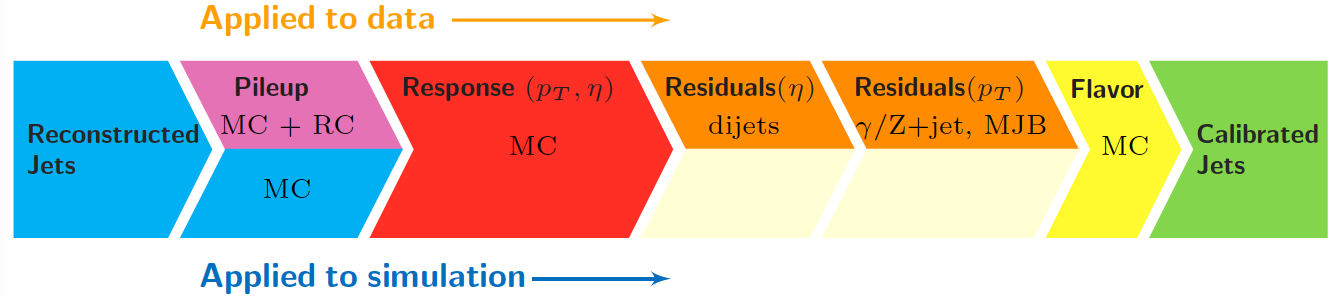
\includegraphics[width=0.9\textwidth]{figuras/Chapter3/JEC_levels.png}
    \caption{Levels of corrections for PF jet four-momentum. Figure taken from \cite{JESandJER}}
    \label{fig:JEC_levels}
  \end{center}
\end{figure}
% Jets are reconstructed with the Particle Flow technique (PF) using the anti$-$k$_{T}$ algorithm \cite{Alwall:2011uj}.
\begin{itemize}
 \item \textbf{Pileup correction}: Also referred as ``L1 correction''. This correction is applied to discard any 
 contribution to the jet reconstruction from PU processes. It corrects for the additional tracks and 
 the excess of energy deposits in the calorimeters due to pileup events. This contribution 
 is estimated using simulated di-jet events with and without PU, and it is 
 parameterized as a function of the offset energy density $\rho$, the jet area, the jet $\eta$-direction 
 and the jet \pt~\cite{JECpileup}. 
 \item \textbf{True response}: The second level of JEC (known as L2L3 MC-truth correction) is related to 
 the detector response and to its effect over the hadron distributions. It corrects for their 
 non-uniformity in the $\eta$ direction and their non-linearity in \pt, by comparing with MC generated 
 distributions in QCD-multijet events. 
 %The jet response is estimated 
 %comparing the distributions momentum of the reconstructed particles and the ones generated by MC in 
 \item \textbf{Residual corrections}: L2L3 residual corrections are applied to address 
 the remaining differences between the jet response on data and MC (of the order of $1 \%$). These corrections are 
achieved with data-driven methods, using di-jet samples for $\eta$-dependent part corrections,
and $\gamma /$Z+jets samples for \pt~part. 
 \item \textbf{Flavor correction}: This is an optional correction, useful for some analyses 
 focused in identifying, at some level, the initial parton of the jet. Since the true 
 response correction is performed using QCD samples with flavor mixture at parton level, this 
 correction assumes a specific flavor hypothesis for the initial parton of the jet and 
 considers the jet response for different initial parton flavors. For example, jets coming
 from light quarks have higher momentum particles than the ones coming from gluons \cite{JecJet}. 
\end{itemize}

% \textbf{\textcolor{red}{DECIR ALGUNA COSA DE CMS RECONSTRUCTION.}}

\noindent The jet reconstruction is important for this analysis, since jets are taken 
as an input in order to reconstruct the hadronic tau decay. In this work, the jet 
reconstruction is performed with the anti-kT algorithm, using the distance 
parameter $\Delta R(\phi,\eta) =$ 0.4. Jets are required 
to have \pt~$>$ 30 \GeV~ and $|\eta| <$ 2.4. For the jet identification, the 
the loose ID working point is used, which has a reconstruction efficiency in simulation greater than 98$\%$. The 
jet energy corrections recommended by the CMS collaboration were applied \cite{JetPOG}.

\section{b-jet Identification}
\label{sec:bJet}

The identification of jets originated from bottom quark decays, or \textit{b-tagging}, exploits 
the properties of the $B$-hadrons, such as their large decay life-times ($c\tau~$450 $\mu$m), which 
leads to displaced tracks as well as the presence of leptons in the final state 
coming from semileptonic decays. CMS has developed several algorithms for b-jet 
identification \cite{bjetID} based on features such as the large 
impact parameter of the b-jet candidate, with respect to the primary vertex;
%of charged particle tracks, 
a possible secondary vertex reconstructed inside the jet; the mass
and the number of tracks associated to the secondary vertex; the number of tracks in 
the jet and the possible presence of soft leptons. In this analysis we use the 
Combined Secondary Vertex algorithm (CSV), which shows the best 
performance for b-jet identification \cite{bjetperformance}. The CSV algorithm is based on a 
MultiVariate Analysis (MVA), combining the information
of  displaced tracks, secondary vertices and the jet kinematics. The method
provides a single discriminator to evaluate the compatibility of a given jet 
with a b-jet. The CSV discriminator defines three possible working points:
the CSVL, or loose working point, allows to select a high 
b-tagging efficiency; the CSVT, or tight working point, 
allows to select a high purity b-jet sample; and 
the CSVM, or middle working point, shows a high efficiency preserving 
high purity. The three working points have been defined 
according to their b-tagging misidentification rate (probability of a non b-jet being 
tagged as a b-jet) and their b-tagging efficiency (probability of a real b-jet being tagged 
by the algorithm). Table \ref{table:b-tagWP} shows the b-tagging efficiency for the three working points.\\
%\ref{table:b-tagWP} shows the b-tagging misidentification rate and the b-tagging efficiency
%for the three working points.\\

\begin{table}[ht]%[!Hhtbp]
\centering{
% TABLA CON MISTAG PROBABILITY FOR RUN I... NECESITA SER ACTUALIZADA
%  \begin{tabular}{ | c | c | c | c |} \hline 
%             \textbf{Working Point} & \textbf{CSVv2 discriminator} & \textbf{Mistag probability}  & \textbf{b-tagging efficiency} \\ \hline \hline
%	      Loose                 & $\geq$ 0.460               & 10 $\%$                      &  $\approx$ 83 $\%$ \\ \hline
%	      Medium                & $\geq$ 0.800               & 1 $\%$                       &  $\approx$ 69 $\%$ \\ \hline
%	      Tight                 & $\geq$ 0.935               & 0.1 $\%$                     &  $\approx$ 49 $\%$ \\ \hline
%  \end{tabular}
  \begin{tabular}{ | c | c | c |} \hline 
             \textbf{Working Point} & \textbf{CSVv2 discriminator}   & \textbf{b-tagging efficiency} \\ \hline \hline
	      Loose                 & $\geq$ 0.5426                   &  $\approx$ 83 $\%$ \\ \hline
	      Medium                & $\geq$ 0.8484                   &  $\approx$ 69 $\%$ \\ \hline
	      Tight                 & $\geq$ 0.9535                   &  $\approx$ 49 $\%$ \\ \hline
  \end{tabular}

\caption{CSVv2 discriminator threshold and corresponding efficiency for the three working points. 
The efficiencies have been determined using b-jets with transverse momentum above 30 \GeV, with simulated $t\bar{t}$ events 
in pp collisions at $\sqrt{s}=13$ \TeV. The numbers are presented just for illustration since they also depend 
on the $p_{T}$ and $\eta$ distributions of the jets \cite{bjetWP}.\label{table:b-tagWP}}
}
\end{table}

\noindent The b-tagging algorithm has been improved for Run II (CSVv2) with the main aim of reducing
the computing time. CVSv2 includes an updated multivariate algorithm that estimates the CSV discriminator
using a neural network method instead of a simple likelihood rate method; besides, it also uses a 
new algorithm for the secondary vertex reconstruction (Inclusive Vertex Finder, IVF) as well as   
an improved track selection. The improvement of the CSVv2 algorithm lead to an increase of about 10$\%$ in 
the b-jet identification efficiency compared to the CSV algorithm used for Run I 
(see Figure \ref{fig:bjetRun1vsRun2}) \cite{PerformancebJetjetmet}. The loose working point, which provides an 
efficiency of 83$\%$, is used in this analysis.

\begin{figure}[ht]%[!Hhtbp]
  \begin{center}
    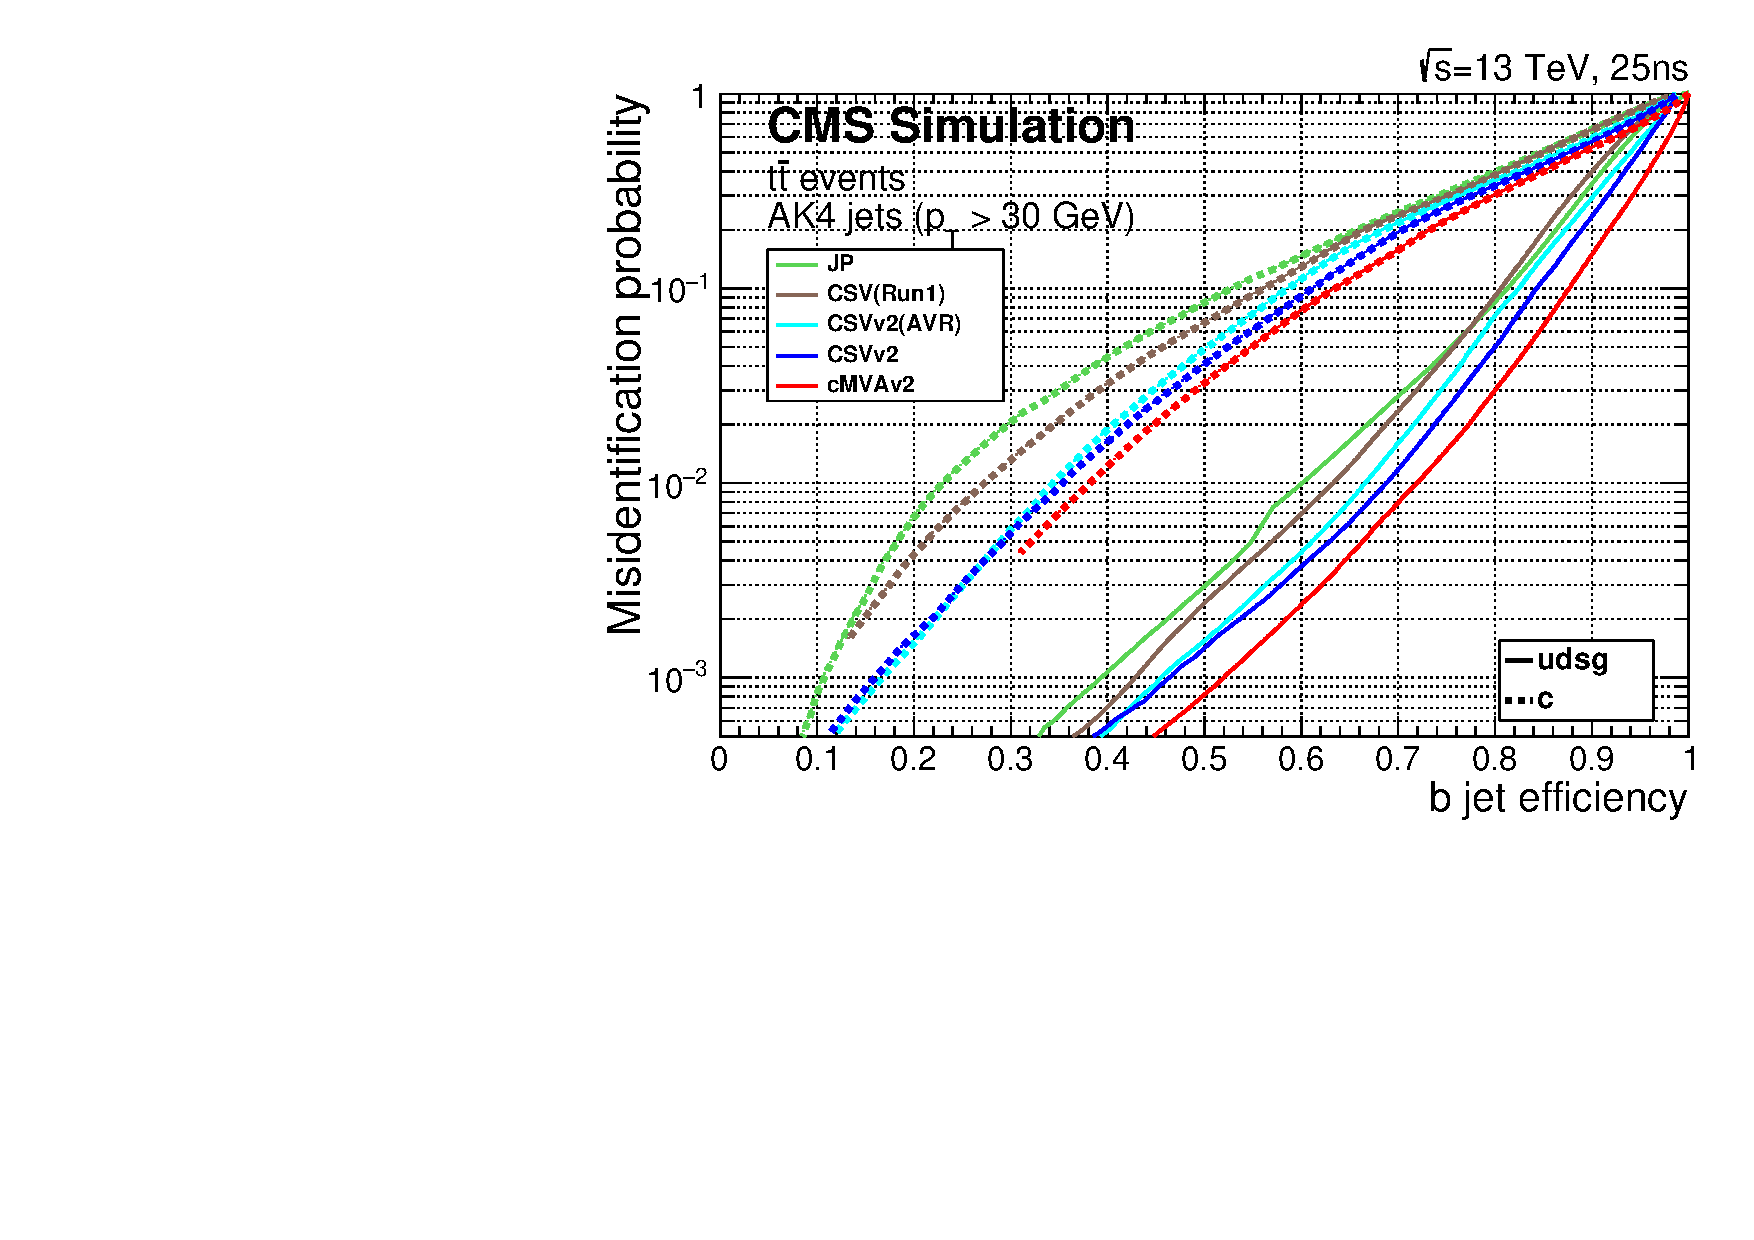
\includegraphics[width=0.6\textwidth]{figuras/Chapter3/bjet_performance_algos.pdf}
    \caption{Efficiency of non-b jets to be misidentified as b-jet, as a function of the b-jet efficiency 
	     for several jet-identification algorithms. An enriched $t\bar{t}$ sample with 2.6 fb$^{-1}$ 
	     from the data collected in 2015 at $\sqrt{s}=13$ \TeV~and a BX of 25 ns. Although cMVAv2 algorithm 
             shows the best performance, the CSVv2 algorithm is used for many analysis and shows 
             an improvement compared with the CSV algorithm used in Run I. Figure taken from \cite{bjetWP}}
    \label{fig:bjetRun1vsRun2}
  \end{center}
\end{figure}


\section{Missing Transverse Energy}
\label{sec:MET}

Almost all the final states coming from a pp collision 
can be detected and identified by the CMS experiment
with the exception of neutral particles, that only interact
weakly with matter, such as neutrinos or hypothetical 
neutralinos. Although these particles scape from CMS without detection, it is possible 
to infer the transverse momenta carried by all of them using the 
transverse momentum conservation. The transverse momentum carried 
out by all the weakly interacting particles, known as the missing 
transverse momentum, and denoted by \METv, is determined by the total 
momentum imbalance of the event in the orthogonal plane to the beam 
line. There are several algorithms for the \METv~reconstruction 
in CMS \cite{METPerformance}; the most common are: the PF \METv~algorithm 
which is based on the PF technique  and the Calo-\METv~algorithm which uses only
the energy deposited in the calorimeter towers. The PF \METv~reconstruction is widely 
used by the CMS analyses, and it is defined as the negative of the 
vectorial sum of transverse momenta of all PF particles. Its 
magnitude is known as missing transverse energy (MET or \MET):

\begin{equation} \label{eq:MET}
\begin{aligned}
\not\!\!\vec{E}_T &= -  \sum_{i \; \epsilon \; tracks} \vec{\textrm{p}}_{\textrm{T}, i} \; , \\
\not\!\!E_T &= \left| \not\!\!\vec{E}_T \right| \;.
\end{aligned}
\end{equation}

\noindent Similar to the case of the jet reconstruction, the missing transverse momentum
can be overestimated due to experimental effects such 
as the pileup and the non-linearity and non-uniformity of the detector response to 
hadrons (see Section \ref{sec:Jet}). With the purpose to address this overestimation, 
three kinds of corrections can be applied to the \METv~measurement:

\begin{itemize}
 \item \textbf{Type-0 Correction}: the purpose of this correction is to remove any contribution 
 from PU interactions to \METv. Although, PU processes produce few invisible particles (mainly
 neutrinos coming from kaon decays), they degrade the \METv~estimation due to the incapability
 to identify all the tracks coming from PU interaction. In consequence, this correction 
 removes all charged hadrons that might come from pile-up interactions from the \METv~estimation.
  \item \textbf{Type-I Correction}: this correction includes the JEC for the jets, in the 
  \METv~reconstruction. All the particles that can be clustered into jets are identified 
  and their momenta are replaced with the sum of the transverse momenta of the 
  jets that include JEC \cite{METPerformance2}. The correction is given by:
  \begin{equation}
  \label{eq:METcorrection}
  \not\!\!\vec{E}_T^{corr} =~\not\!\!\vec{E}_T - \sum_{jets} \left( \vec{\textrm{p}_{\textrm{T,}}}_{\textrm{jets}}^{JEC} - \vec{\textrm{p}_{\textrm{T,}}}_{\textrm{jets}} \right)
\end{equation} 
 
 \item \textbf{xy-Shift Correction}: the \MET~measurement should be independent of the $\phi$-direction,
 due to the cylindrical symmetry of the CMS detector. However, a dependency on $\phi$ is observed, which 
 might come from anisotropic detector responses, inactive calorimeter cells or detector 
 misalignments. Besides, the $\phi$ dependency on \MET~is also related with the pileup
 contributions and can be mitigated by shifting the origin of the transverse momentum plane.
\end{itemize}

\noindent The ``type-I'' correction to \METv~is widely preferred by CMS analyses. For Run II, 
the ``type-I'' correction requires jets with \pt~greater than 15 \GeV~(including JEC) whose  
energy fraction deposited in the ECAL is less than 0.9 \cite{METPerformance2}. \\

\noindent The performance of \MET  ~reconstruction is estimated from Z bosons
in di-lepton events. The \MET~resolution is dominated by the hadron activity 
in the event since the leptons have high momentum resolution, which varies 
from 1-6$\%$ for muons, 1-4$\%$ for electrons$/$photons and 5-15$\%$ for 
jets. Figure \ref{fig:MetPerfomance} shows a very good agreement between data and 
simulated events for the \MET~distribution in the $Z\rightarrow \mu^{-}\mu^{+}$ 
and $Z\rightarrow e^{-}e^{+}$ channels \cite{METPerformance2}.\\
 
\begin{figure}[ht]
  \begin{center}
    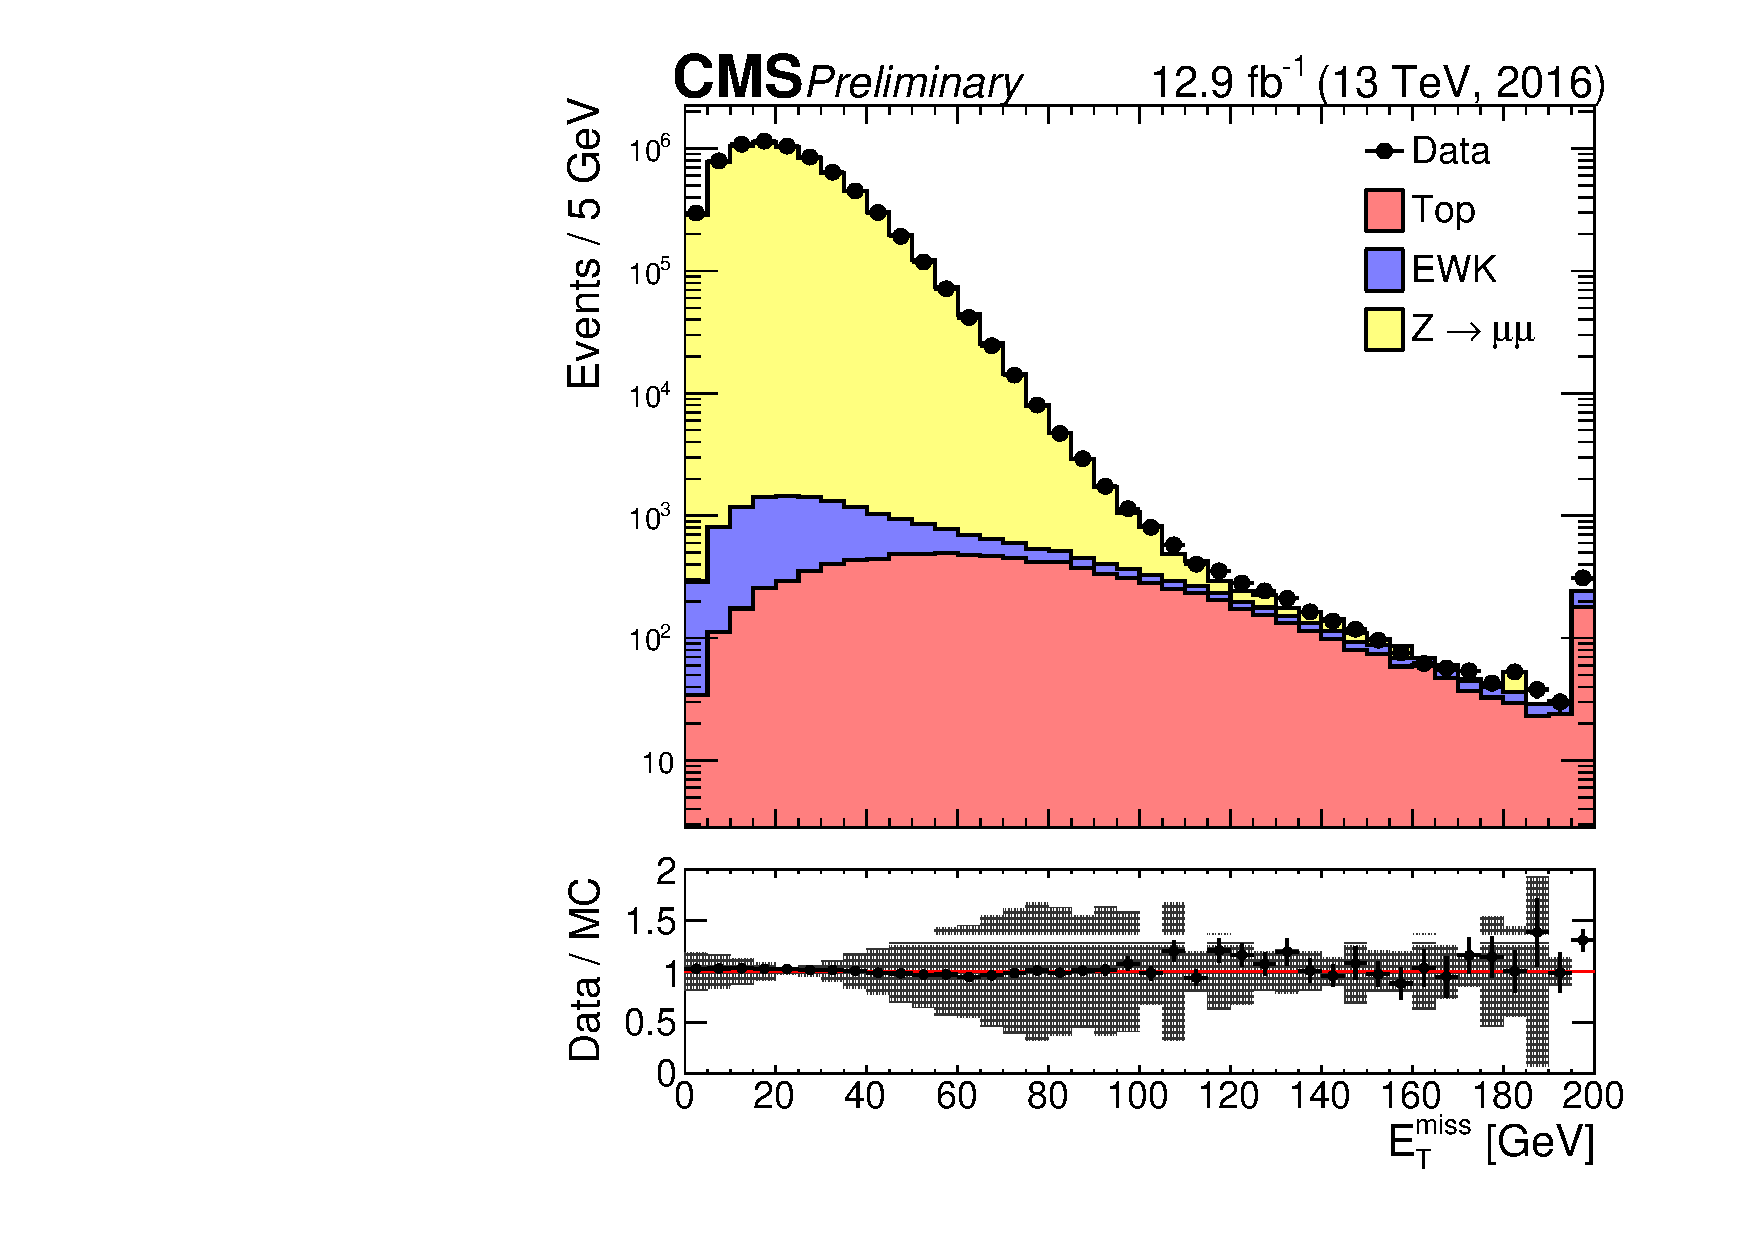
\includegraphics[width=0.43\textwidth]{figuras/Chapter3/METPerformancemumu.pdf}
    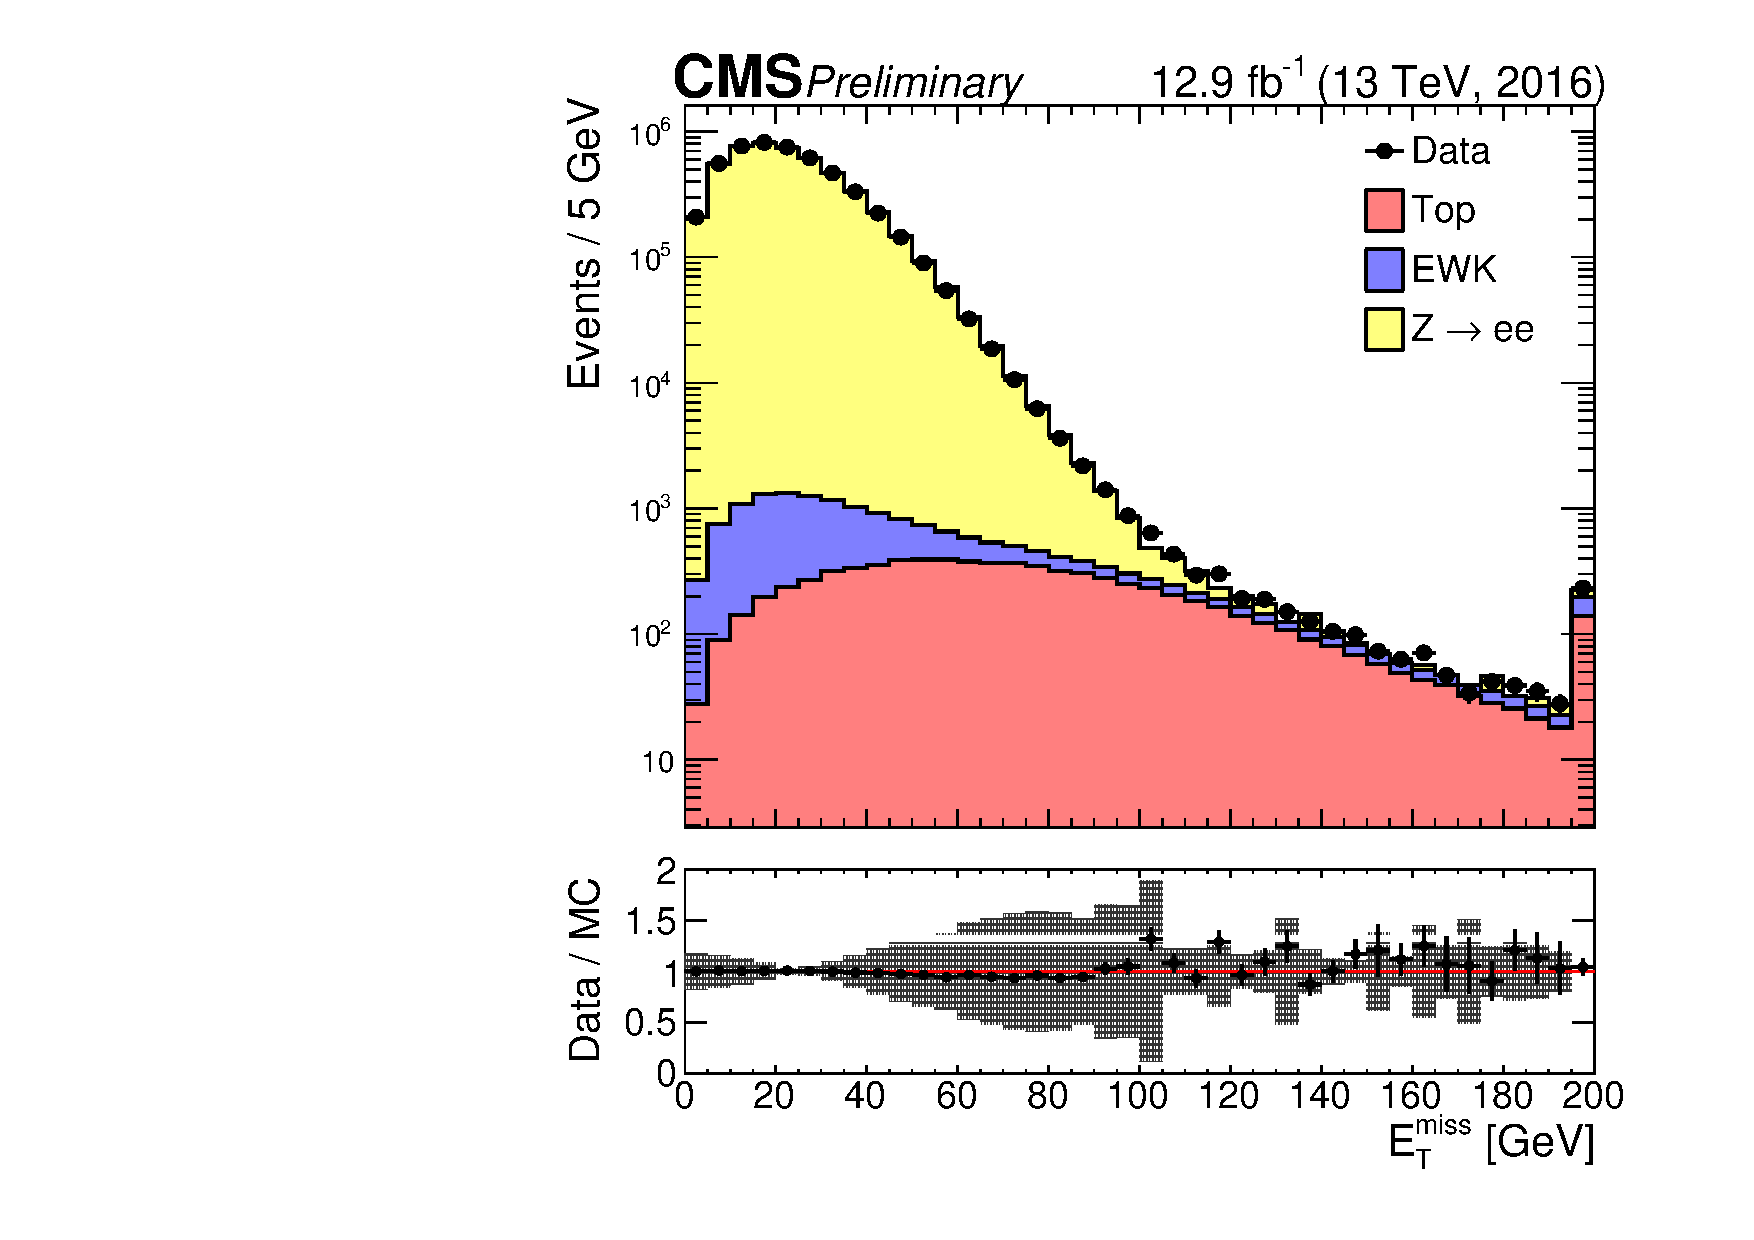
\includegraphics[width=0.43\textwidth]{figuras/Chapter3/METPerformanceee.pdf}
    \caption{\MET~distribution for $Z\rightarrow \mu^{-}\mu^{+}$ (left) and $Z\rightarrow e^{-}e^{+}$ (right). Data comes 
    from pp collisions at \sqrts 13 \TeV~ collected by CMS detector during 2016 (integrated luminosity up to 12.9 fb$^{-1}$).
    Figure taken from \cite{METPerformance2}.}
    \label{fig:MetPerfomance}
  \end{center}
\end{figure} 

\noindent In this analysis, the ``type-I'' correction to \METv~is applied. In order to reject 
any anomalous event with high-\MET, the filters recommended by the CMS Collaboration
were applied \cite{METPOG}. 

\section{Tau Reconstruction and Identification}
\label{sec:RecoTau}

As was mentioned in section \ref{sec:Taus}, the leptonic decays of the tau
cannot be distinguished from the leptons originated in the hard interaction and,
therefore, only the hadronic decays can be identified directly. The hadronic tau 
reconstruction is challenging, from the experimental point of view, since its
signature is pretty similar to the one of a QCD-jet, which is produced 
with a cross section eight order of magnitude larger. Additionally, 
the tau kinematic variables cannot be fully reconstructed due to the presence
of neutrinos in its decay modes. In most of the CMS analyses, the 
tau reconstruction and identification is performed 
using the \textit{Hadron-Plus-Strips} algorithm (HPS)\cite{CMS-PAS-TAU-16-002}. This 
algorithm has two stages:

\begin{itemize}
 \item \textbf{Reconstruction}: The algorithm searches for 
 charged and neutral PF objects that are compatible with the tau-decay modes, 
 in order to reconstruct a tau and to compute its kinematic variables.
 \item \textbf{Identification}: Discriminators are applied on the 
 reconstructed tau in order to distinguish it from background processes,
 such as QCD jets, electrons and muons, reducing the misidentification rates.
\end{itemize}

\subsection{Tau Reconstruction Algorithm}
\label{subsec:HPS}

 The HPS algorithm takes as input jets reconstructed with the anti-kT algorithm 
 (described in section \ref{sec:Jet}) and reconstructs individually the 
 hadronic tau decay modes, using the charged and neutral constituents of the jet 
 built by the PF algorithm. As can be seen in Table \ref{tab:taumodescomplete}, the 
 hadronic decays are composed by one neutrino, neutral pions and charged hadrons (mostly pions).
 In consequence, the HPS algorithm looks for charged hadrons  using the information 
 provided by the Tracker and Calorimeter Systems, and looks for energy deposits 
 in the calorimeters consistent with the signature of neutral pions. As was mentioned 
 in section \ref{sec:Tracker}, there is a high probability that a photon, coming from a 
  $\pi^{0} \rightarrow \gamma\gamma$ decay, can convert into 
  an electron-positron pair due to its interaction
 with the Tracker material; then, the electron and the positron 
 are  spread apart in opposite directions due to the bending of their tracks by 
 the magnetic field, resulting in energy deposits 
 enlarged in the $\phi$-direction (see Figure \ref{fig:taudecays2}). Therefore, 
 the HPS algorithm looks for ECAL strips in the $\eta-\phi$ plane 
 consistent with the \picero~signature. These strips are combined 
 with the charged hadrons with the aim to reconstruct 
 the possible tau decay modes. \\
 
\begin{table}[ht]
\begin{center}
\begin{tabular}{|l|c|c|c|}
  \hline \hline 
  Final State                                            &  Branching Fraction [$\%$] &  Resonance & Mass [\GeV]   \\ \hline\hline
   $e^{-}\bar{\nu}_{e}\nu_{\tau}$                        & 17.8                    &            &   \\ \hline
   $\mu^{-}\bar{\nu}_{\mu}\nu_{\tau}$                    & 17.4                    &            &   \\ \hline \hline 
   $h^{-}\nu_{\tau}$                                     & 11.5                    &            &   \\ \hline
   $h^{-}\pi^{0}\nu_{\tau}$                              & 25.9                    & $\rho$     & 770 \\ \hline
   $h^{-}\pi^{0}\pi^{0}\nu_{\tau}$                       &  9.5                    & $a_{1}$    & 1200  \\ \hline
%    $h^{-}\pi^{0}\pi^{0}\pi^{0}\nu_{\tau}$                &  1.0                    &            &   \\ \hline
   $h^{-}h^{+}h^{-}\nu_{\tau}$                           &  9.8                    & $a_{1}$    & 1200  \\ \hline
   $h^{-}h^{+}h^{-}\pi^{0}\nu_{\tau}$                    &  4.8                    & $a_{1}$    & 1200  \\ \hline
   Others                                                &  3.3                    &            &       \\ \hline 
   
%   $e^{-}\bar{\nu}_{e}\nu_{\tau}$                          & 17.83 $\pm$ 0.04          &            &   \\ \hline
%   $\mu^{-}\bar{\nu}_{\mu}\nu_{\tau}$                      & 17.41 $\pm$ 0.04          &            &   \\ \hline \hline 
%   $\pi^{-}\nu_{\tau}$                                     & 10.83 $\pm$ 0.06          &            &   \\ \hline
%   $\pi^{-}\pi^{0}\nu_{\tau}$                              & 25.52 $\pm$ 0.09          & $\rho$     & 770 \\ \hline
%   $\pi^{-}\pi^{0}\pi^{0}\nu_{\tau}$                       &  9.30 $\pm$ 0.11          & $a_{1}$    & 1200  \\ \hline
%   $\pi^{-}\pi^{0}\pi^{0}\pi^{0}\nu_{\tau}$                &  1.05 $\pm$ 0.07          &            &   \\ \hline
%   $\pi^{-}\pi^{-}\pi^{+}\nu_{\tau}$                       &  8.99 $\pm$ 0.06          & $a_{1}$    & 1200  \\ \hline
%   $\pi^{-}\pi^{-}\pi^{+}\pi^{0}\nu_{\tau}$                &  2.70 $\pm$ 0.08          & $a_{1}$    & 1200  \\ \hline \hline 
  \hline
\end{tabular}
\end{center}
 \caption{Branching fraction of $\tau^{-}$ modes \cite{bib:PDG}.}\label{tab:taumodescomplete}
\end{table}


\begin{figure}[ht]
  \begin{center}
    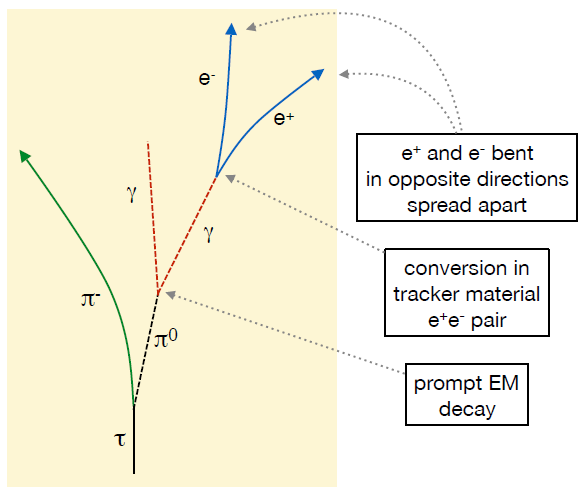
\includegraphics[width=0.53\textwidth]{figuras/Chapter3/taudecays2.png}
    \caption{Schematic view of the $\pi^{-}\pi^{0}\nu_{\tau}$ final state, which represents the 57$\%$ of all hadronic tau decays.}
    \label{fig:taudecays2}
  \end{center}
\end{figure} 

\begin{itemize}
 \item \textbf{Strip reconstruction}. \\

The electrons and photons constituents of the jet, which is used as an input 
for the \tauh~reconstruction, are clustered into $\Delta\eta \times \Delta\phi$ 
strips. The clustering starts with an iterative procedure in order to select 
the highest-\pt~electron, or photon, that has not been included yet in any 
strip; the $e/\gamma$ selected seeds the clustering algorithm. The position of 
the new strip corresponds to the $\eta$ and the $\phi$ positions of the 
$e/\gamma$~seed. Then, the next-larger \pt~electron ,or photon, is 
added to the strip, if it is within an $\Delta\eta \times \Delta\phi$ window. 
The iterative procedure ends when no electrons, nor photons, are found
within the size of the window. In the previous versions of the HPS algorithm,
the size of the $\Delta\eta \times \Delta\phi$ window was fixed to 0.05 $\times$ 0.20 in the $\eta-\phi$ 
plane \cite{TauReconstructionCMSRun1}. In some cases, all 
electrons and photons originated from the tau decay products are not 
included in the fixed size window, reducing the isolation efficiency. For instance,
a charged pion, coming from a \tauh~decay, can produce secondary 
low-\pt~particles due to its nuclear interaction with the tracker 
material, resulting in low-\pt~electrons and photons 
that can lie outside of the window. Therefore, it 
might be convenient to increase the window size, but it would represent a 
decrease in the isolation efficiency for high-\pt~taus, since 
their decay products tend to be boosted and localized into a smaller strip size. In 
consequence, a dynamic-strip reconstruction algorithm has been 
developed based on these considerations (see Figure \ref{fig:StripReco}). \\

\begin{figure}[ht]
  \begin{center}
    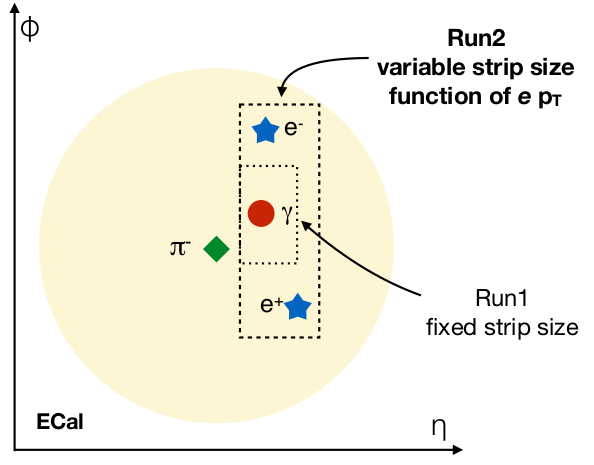
\includegraphics[width=0.53\textwidth]{figuras/Chapter3/StripReco.png}
    \caption{Representation of strip size definition during Run I and Run II.}
    \label{fig:StripReco}
  \end{center}
\end{figure} 

\noindent The dynamic-strip reconstruction selects iteratively the 
next-larger \pt~electron, or photon, and adds it to the strip, if 
it is within a range of:

\begin{equation} \label{eq:windowsize}
 \begin{aligned}
  \Delta\eta &= 0.20 \cdot \frac{(\textrm{p}_{\textrm{T},e/\gamma})^{-0.66}}{\textrm{GeV}} + 0.20 \cdot \frac{(\textrm{p}_{\textrm{T},strip})^{-0.66}}{\textrm{GeV}}  \;, \\
  \Delta\phi &= 0.35 \cdot \frac{(\textrm{p}_{\textrm{T},e/\gamma})^{-0.71}}{\textrm{GeV}} + 0.35 \cdot \frac{(\textrm{p}_{\textrm{T},strip})^{-0.71}}{\textrm{GeV}}  \;,
  \end{aligned}
\end{equation}

\noindent where $\textrm{p}_{\textrm{T},e/\gamma}$ is the $e/\gamma$-momentum and 
$\textrm{p}_{\textrm{T},strip}$ is the momentum associated to the strip. The window size is 
constrained up to 0.15 in $\Delta\eta$ and up to 0.3 
in $\Delta\phi$. As can be inferred from the equations \ref{eq:windowsize}, 
the window size depends on the momentum of both, the strip and the added
electrons or photons. This results in an improvement in the 
isolation efficiency compared to the fixed window size used in Run I,
since it reduces the QCD contamination. Then, 
the strip position is recalculated using a \pt-weighted average of all
electrons and photons included in the strip, as follows:

\begin{equation} \label{eq:stripposition}
 \begin{aligned}
  \eta_{strip} &=  \frac{1}{\textrm{p}_{\textrm{T},strip}} \sum \left(\textrm{p}_{\textrm{T},e/\gamma} \cdot \eta_{e/\gamma}\right) \;, \\
  \phi_{strip} &=  \frac{1}{\textrm{p}_{\textrm{T},strip}} \sum \left(\textrm{p}_{\textrm{T},e/\gamma} \cdot \phi_{e/\gamma}\right) \;,
  \end{aligned}
\end{equation}

\noindent where $\textrm{p}_{\textrm{T},strip} = \sum \textrm{p}_{\textrm{T},e/\gamma}$. The strip reconstruction
ends if no electrons, nor photons, are found within the window. In that case, the clustering 
looks for the highest-\pt~electron, or photon, which is not associated to any strip, and selects it 
in order to reconstruct a new strip. \\

\noindent Strips, whose \pt~is larger than 2.5 \GeV, are kept as \picero~candidates. A 
\picero~candidate can be identified as a tau decay product if the strip position 
is within the signal cone associated to the tau candidate.
 
 \item \textbf{Charged hadron reconstruction}. \\

\noindent As was mentioned above, the constituents of the jet are taken as input for the HPS algorithm,
which looks for charged hadrons consistent with the tau signature. The algorithm
requires charged particles with \pt~larger than 0.5 \GeV, whose transverse impact 
parameter, $d_{xy}$, is less than 0.1 cm. The \pt~requirement on the hadrons ensures 
the selection of high quality tracks, which have a reconstruction efficiency 
of $\sim$95$\%$, and have passed previous requirements, such as the number of reconstructed 
hits on the Tracker System and the $\chi^{2}$ of the fit 
(see Section \ref{subsec:TrackReco}). The criterion on the transverse impact
parameter reduces the background contamination coming from PU and spurious tracks; however, such 
criterion is not so restrictive in order to avoid any rejection of high-\pt~taus, which
would have a long lifetime. 
\end{itemize}

\noindent The set of charged hadrons and strips obtained from the PF jet are 
combined in order to reconstruct the tau decay modes individually. The visible tau decay
products are mainly one or three hadrons plus neutral pions. The 
algorithm aim is to reconstruct all the hadronic decay modes with 
exception of h$^{\pm}$h$^{\mp}$h$^{\pm}$\picero; this decay mode 
is not considered currently by the algorithm because, besides of its
relative low branching ratio ($4.8\%$), it has a significant
background contribution from QCD-jets. In summary, the reconstructed 
decay modes are: h$^{\pm}$, h$^{\pm}$\picero, h$^{\pm}$\picero\picero, 
and h$^{\pm}$h$^{\mp}$h$^{\pm}$ (see Table \ref{tab:taumodescomplete}). \\

\noindent There are three requirements on the hadron plus strip combination
in order to reconstruct the tau candidate: 

\begin{enumerate}
 \item A mass criterion is applied since the tau candidate mass ($m_{\tau}$) must be consistent with the 
 mass of either of the resonances, $\rho$ or $a_{1}$. The mass is optimized for each decay mode
in order to increase the reconstruction efficiency; the requirements are \cite{CMS-PAS-TAU-16-002}:
\begin{itemize}
\item a mass window of 
$(0.3~\textrm{GeV}-\Delta m_{\tau}) < m_{\tau} < (1.3~\textrm{GeV}\cdot\sqrt{\textrm{p}_{\textrm{T}} (\textrm{GeV})} + \Delta m_{\tau})$
 for the h$^{\pm}$\picero~decay mode. The mass upper limit is constrained further to be between 1.3 to 4.2 \GeV;
 \item a mass window of 
 $(0.4~\textrm{GeV}-\Delta m_{\tau}) < m_{\tau} < (1.2~\textrm{GeV}\cdot\sqrt{\textrm{p}_{\textrm{T}} (\textrm{GeV})} + \Delta m_{\tau})$
%  0.4 \GeV$-\Delta m_{\tau} < m_{\tau} < 1.2$ \GeV~$\cdot \sqrt{\textrm{p}_{\textrm{T}} (\textrm{GeV})} + \Delta m_{\tau}$
 for the h$^{\pm}$\picero\picero~ decay mode. The mass upper limit is constrained further to be between 1.2 to 4.0 \GeV;
 \item a mass window of
 $0.3~\textrm{GeV} < m_{\tau} < 1.3~\textrm{GeV}\cdot\sqrt{\textrm{p}_{\textrm{T}} (\textrm{GeV})}$ 
%  0.3 \GeV$< m_{\tau} <$ 1.3 \GeV~$\cdot \sqrt{\textrm{p}_{\textrm{T}} (\textrm{GeV})}$ 
 for the h$^{\pm}$h$^{\mp}$h$^{\pm}$ decay mode. The mass upper limit is constrained further to be between 1.3 to 4.2 \GeV. \\

 
 
 \end{itemize}
\noindent where $\Delta m_{\tau}$ corresponds to the mass change due to the addition of $e/\gamma$ candidates 
to the strip reconstruction. 
 \item The electric charge of the tau candidate must be $\pm$ 1, otherwise they will be rejected.
 \item The tau decay products must lie within the signal cone. The signal cone is centered in the 
 direction of the tau momentum, which initially is assumed as the direction of the hadron with highest momentum, and it 
 has a radius of $R_{sig}=3.0 / \textrm{p}_{\textrm{T}} (\textrm{GeV})$, where 
 \pt~corresponds to the sum of the charged hadrons momenta. The lower and upper limits on $R_{sig}$ are
 0.05 and 0.1, respectively.
\end{enumerate}

\noindent When multiple decay modes pass the tau requirements described above for the input jet, 
only the hypothesis with the highest-\pt~is selected. Then, a single 
tau candidate is reconstructed for each jet. The 4-momentum of the \tauh~candidate
is the sum of the 4-momenta of the charged hadrons and the one 
reconstructed from the strips.\\

\textbf{Decay Mode Reconstruction}\\

\noindent In the tau reconstruction jargon, the number of charged particles in a 
tau decay mode is known as \textit{prong}. Hereafter, the decay modes will 
be referred as:
\begin{itemize}
 \item \textbf{1 prong}: for h$^{\pm}$.
 \item \textbf{1 prong + \picero}: for h$^{\pm}$\picero and h$^{\pm}$\picero\picero.
 \item \textbf{3 prongs}: for h$^{\pm}$h$^{\mp}$h$^{\pm}$.
\end{itemize}

\begin{figure}[ht]
  \begin{center}
    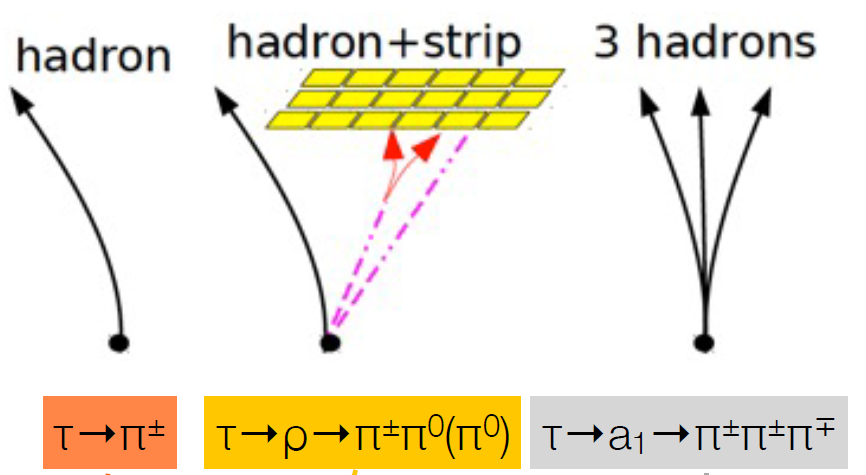
\includegraphics[width=0.5\textwidth]{figuras/Chapter3/taudecays.png}
    \caption{Tau decay modes reconstructed by the HPS algorithm.}
    \label{fig:taudecaysReco}
  \end{center}
\end{figure} 

\noindent In the previous version of the HPS algorithm, the decay mode 
reconstruction (\textbf{oldDMF}) only considers the final states listed 
above (see Figure \ref{fig:taudecaysReco}). However, an additional 2-prong unphysical 
final state can be considered, which results from high-\pt~taus in the 3-prong decay mode;
in this case, the tracks of the boosted charged hadrons are very close, 
and the  distance between two of them can be smaller than the spatial resolution 
of the Tracker System. Therefore, two of the three tracks are 
merged and reconstructed as a single charged hadron, resulting in an 
apparent 2-prong final state. In the latest version of the HPS algorithm, the decay mode 
reconstruction (\textbf{newDMF}) also considers the 2-prong final state. For this analysis,
the newDMF was used. The decay modes considered in the tau reconstruction 
affect the sensitivity of the \Zprime~identification, since they are correlated 
with the QCD contamination. The decay modes used for the 
tau reconstruction are 1or3-prongs, instead of 1or2or3-prongs, since a better 
significance is obtained. 

%  In order to reduce the computing time, only the highest-\pt~six charged 
% hadrons and six strips are selected as input.

\subsection{Tau Identification}
\label{subsec:TauIdentification}

\noindent Once the tau candidates are reconstructed, discriminants dedicated
to identify them from each background contamination are applied. As it has 
been mentioned before, jets, muons and electrons can fake the 
tau signature. In this section these discriminator algorithms
are described. 

\subsubsection{Tau Isolation Discriminator}
\label{subsubsec:IsoDiscriminators}

The purpose of the tau isolation discriminator is to reduce the background contribution
from QCD jets. Since the QCD jet energy is carried out by charged hadrons ($\sim65\%$), photons 
from $\pi^{0}$ decays ($\sim15\%$) and neutral hadrons ($\sim20\%$) \cite{CMS-PAS-PFT-10-001},
their signatures are similar to those produced by the hadronic tau decay modes; besides, QCD 
jets have a cross section around eight orders of magnitude larger, making the discrimination
against jets crucial for the \tauh~identification. The isolation discriminator
algorithm mainly exploits two variables that distinguish hadronic taus from 
QCD jets. The first one is the distance between the decay products of a hadronic tau, since 
it is correlated with the tau energy; therefore, the decay products of 
a high-\pt~tau lie within a narrower cone than the constituents of a QCD jet. The 
second one is the multiplicity of the particles, since the hadronic 
taus have few number of particles, each one with high momentum, whereas 
the QCD jet has a higher multiplicity of particles with 
a wider energy profile. For these reasons, the so 
called \textit{isolation-sum discriminator} uses a cone whose size 
should be big enough to contain all the decay products coming 
from the $\tau_{h}$ decay and small enough to reject the QCD events. The 
isolation cone has a size of $\Delta R =$ 0.5 and it 
is centered in the \tauh~direction (see Figure \ref{fig:taucone}). \\

\begin{figure}[ht]
  \begin{center}
    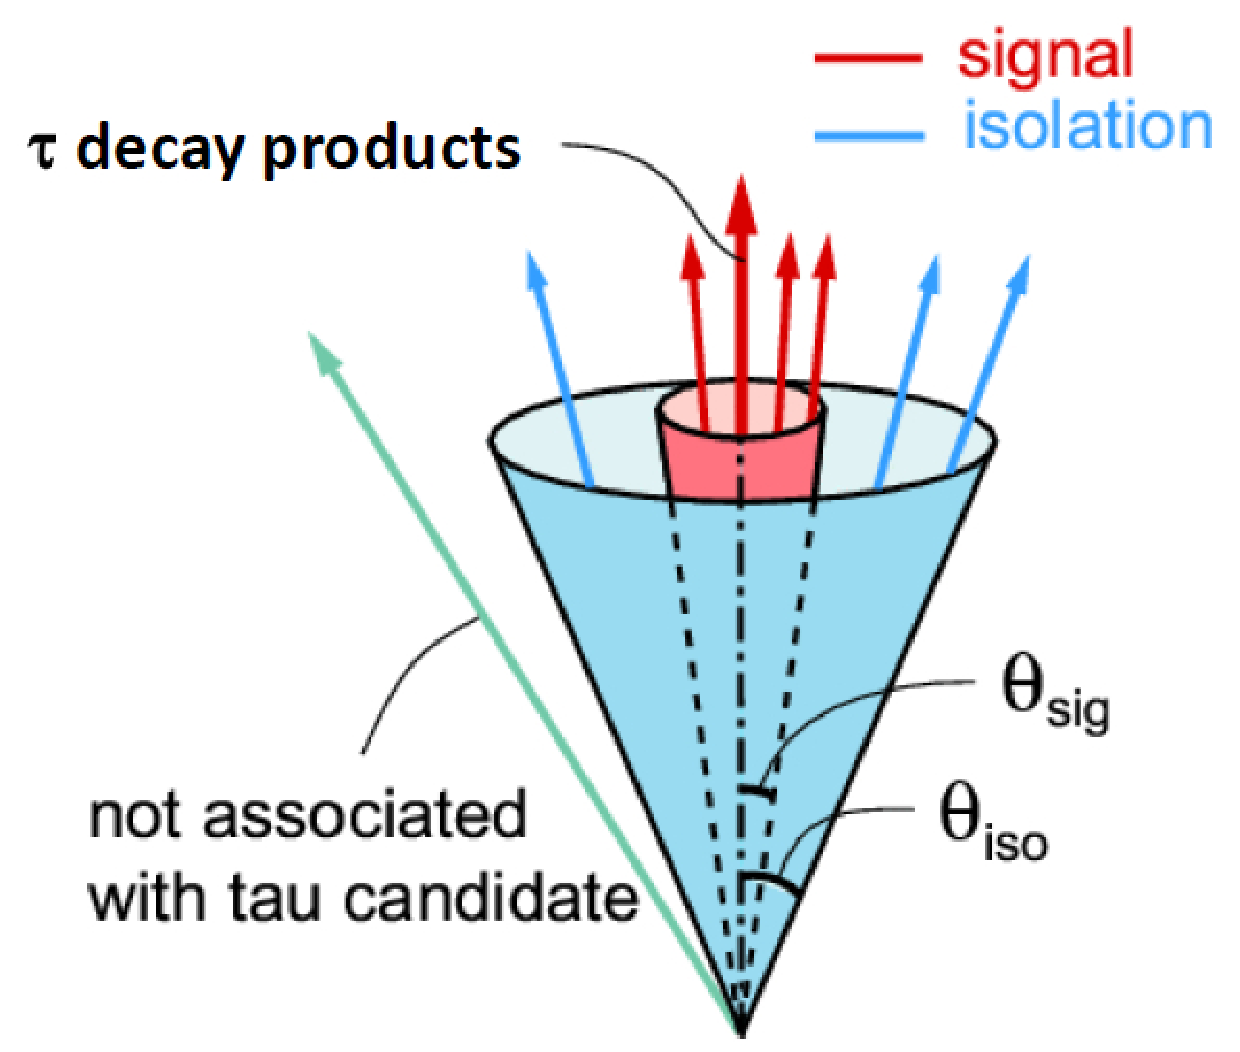
\includegraphics[width=0.48\textwidth]{figuras/Chapter3/taucone}
    \caption{Cone definition for tau  isolation discriminator.}
    \label{fig:taucone}
  \end{center}
\end{figure} 

\noindent The isolation-sum discriminator is computed using all the 
charged particles and photons reconstructed by the PF algorithm that lie 
within the cone, excluding those that are identified
as constituents of the tau candidate. It is defined as:

\begin{equation} \label{eq:TauIso}
I_{\tau} = \sum \textrm{p}_{\textrm{T}}^{charged} (d_{z} < 0.2 \textrm{cm}) + 
max\left(0, \sum \textrm{p}_{\textrm{T}}^{\gamma}- \Delta\beta \sum \textrm{p}_{\textrm{T}}^{charged} (d_{z} > 0.2 \textrm{cm}) \right) \; ,
\end{equation}

\noindent where any contribution coming from PU interactions are suppressed through 
requirements on the production vertex of the charged hadrons ($d_{z}$): 

\begin{itemize}
 %\item The ca PU contribution is suppressed requiring that the charged particles are 
 \item The charged hadrons that come from PU are suppressed, requiring that the tracks are originated 
 in the production vertex of the \tauh~($d_{z} < 0.2 \textrm{cm}$).
 \item The PU contribution to the photon reconstruction is suppressed requiring that the charged 
 particles, within a cone of size $\Delta R =$ 0.8, are not originated in the 
 production vertex  of the \tauh~($d_{z} > 0.2 \textrm{cm}$). The so-called 
 $\Delta \beta$-factor makes the tau efficiency independent of the PU \footnote{
 The $\Delta \beta$-factor is defined as the ratio between the energy of all 
 charged hadrons and the energy of all photons that come from PU.}. For Run II, the  $\Delta \beta$ value used is 0.2.
\end{itemize}

\noindent The loose, medium and tight working points (WP) for the 
isolation-sum discriminant are defined requiring $I_{\tau}$ to be 
less than 2.5 \GeV, 1.5 \GeV, and 0.8 \GeV, 
respectively \cite{CMS-PAS-TAU-16-002}. Figure \ref{fig:IsoSumPerformance} shows 
a comparison of the isolation-sum discriminators' performance for 
the previous and the current versions of the HPS algorithm. As was 
mentioned in the previous section, the main difference between them is
the size used for the strip reconstruction, which was fixed for 
Run I, while for Run II it depends on the \pt~of the electrons and photons
(dynamic-strip reconstruction). The dynamic-strip reconstruction
allows to include the photons (coming from the tau decay products)
that might lie outside of the signal cone, reducing the 
jet $\rightarrow$~\tauh~misidentification rate (see Figure \ref{fig:IsoSumPerformance}). In order to
% compare the performance of the working points (Figure \ref{fig:IsoPerformance}), MC signal
compare the performance of the working points, MC signal 
samples corresponding to $H \rightarrow \tau\tau$ and \Zprimetotautau~events were used, while 
MC background samples corresponding to QCD multijet processes were used. This study 
was performed using pp collisions at \sqrts 13 \TeV. For the current version of the HPS algorithm,
the tight isolation-sum discriminator has a $\tau$~identification efficiency 
of $\sim$60$\%$, and the QCD jet rejection rate is  $\sim$99.7$\%$.\\

\begin{figure}[ht]
  \begin{center}
    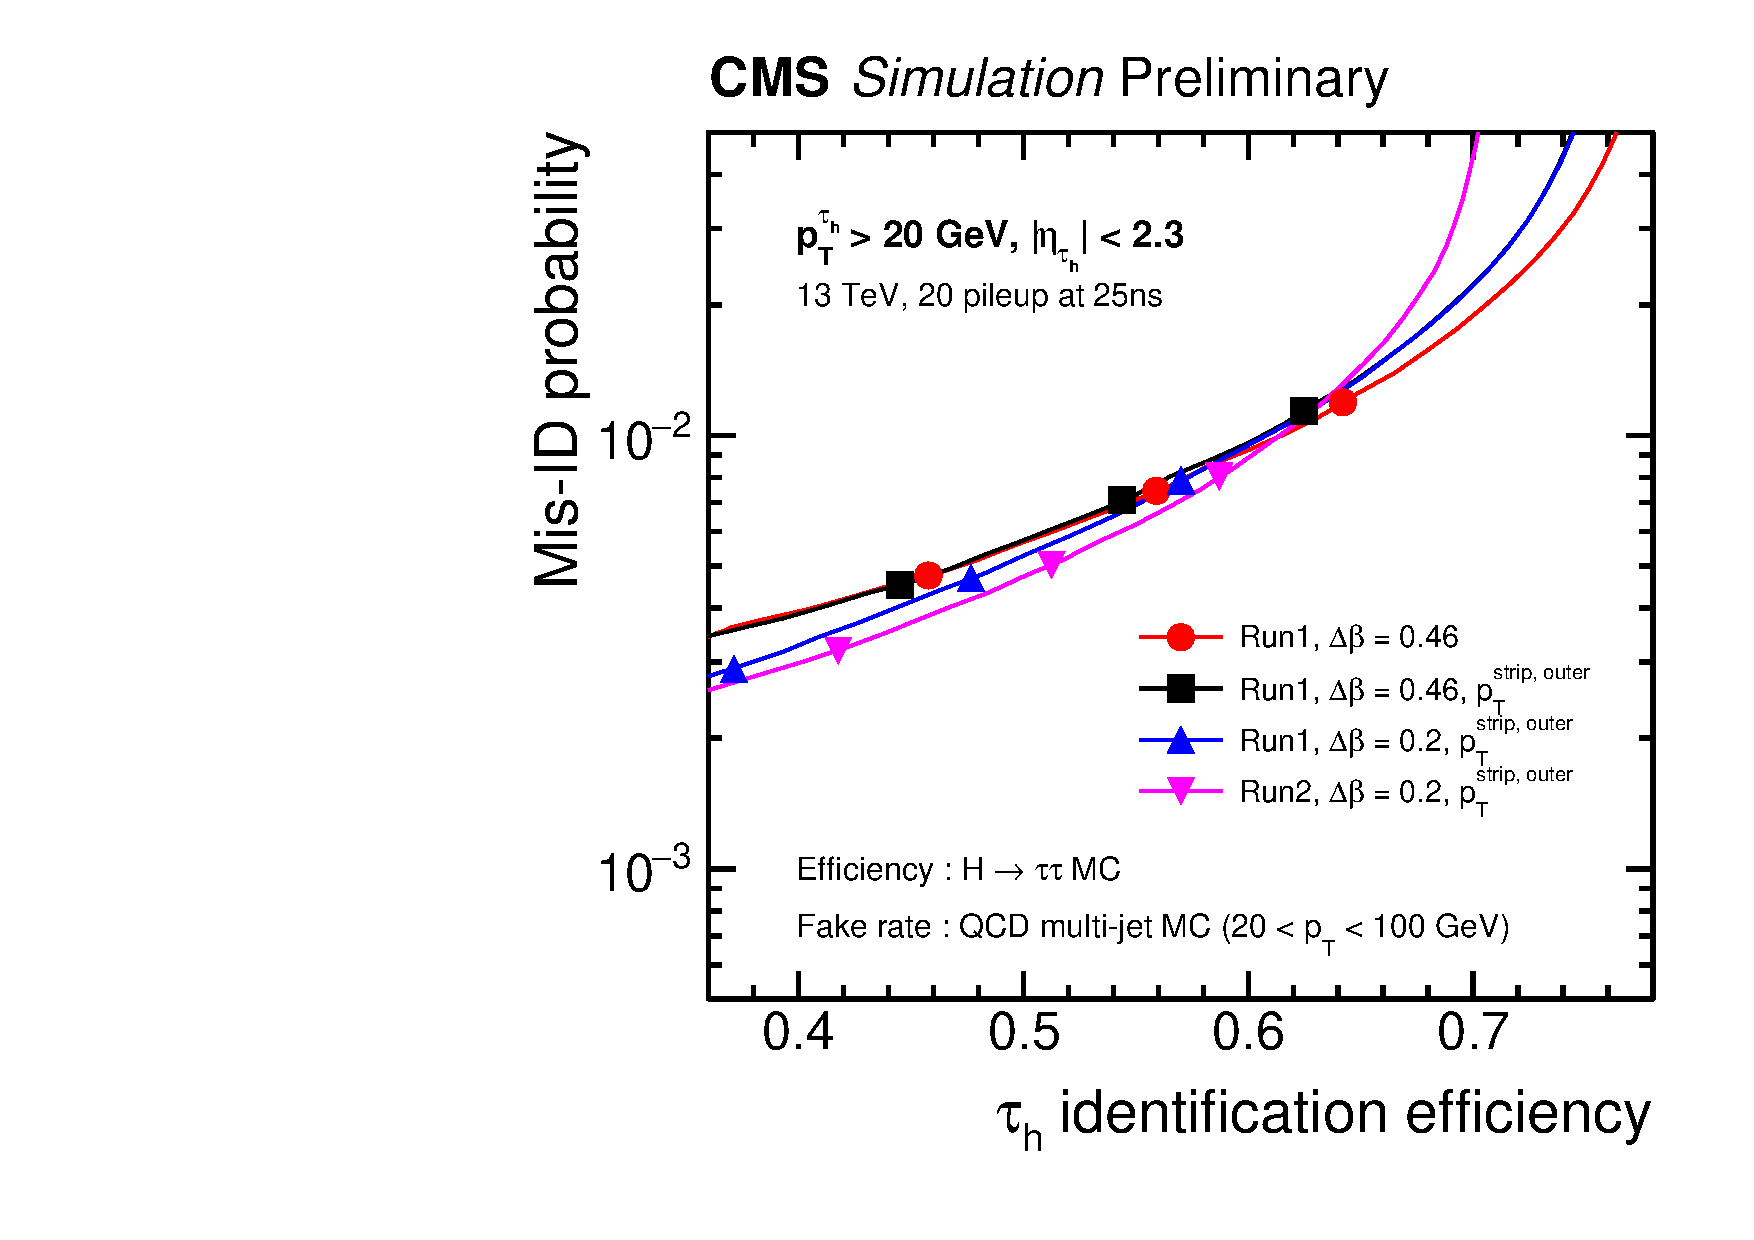
\includegraphics[width=0.4\textwidth]{figuras/Chapter3/IsoPerformanceHiggs}
    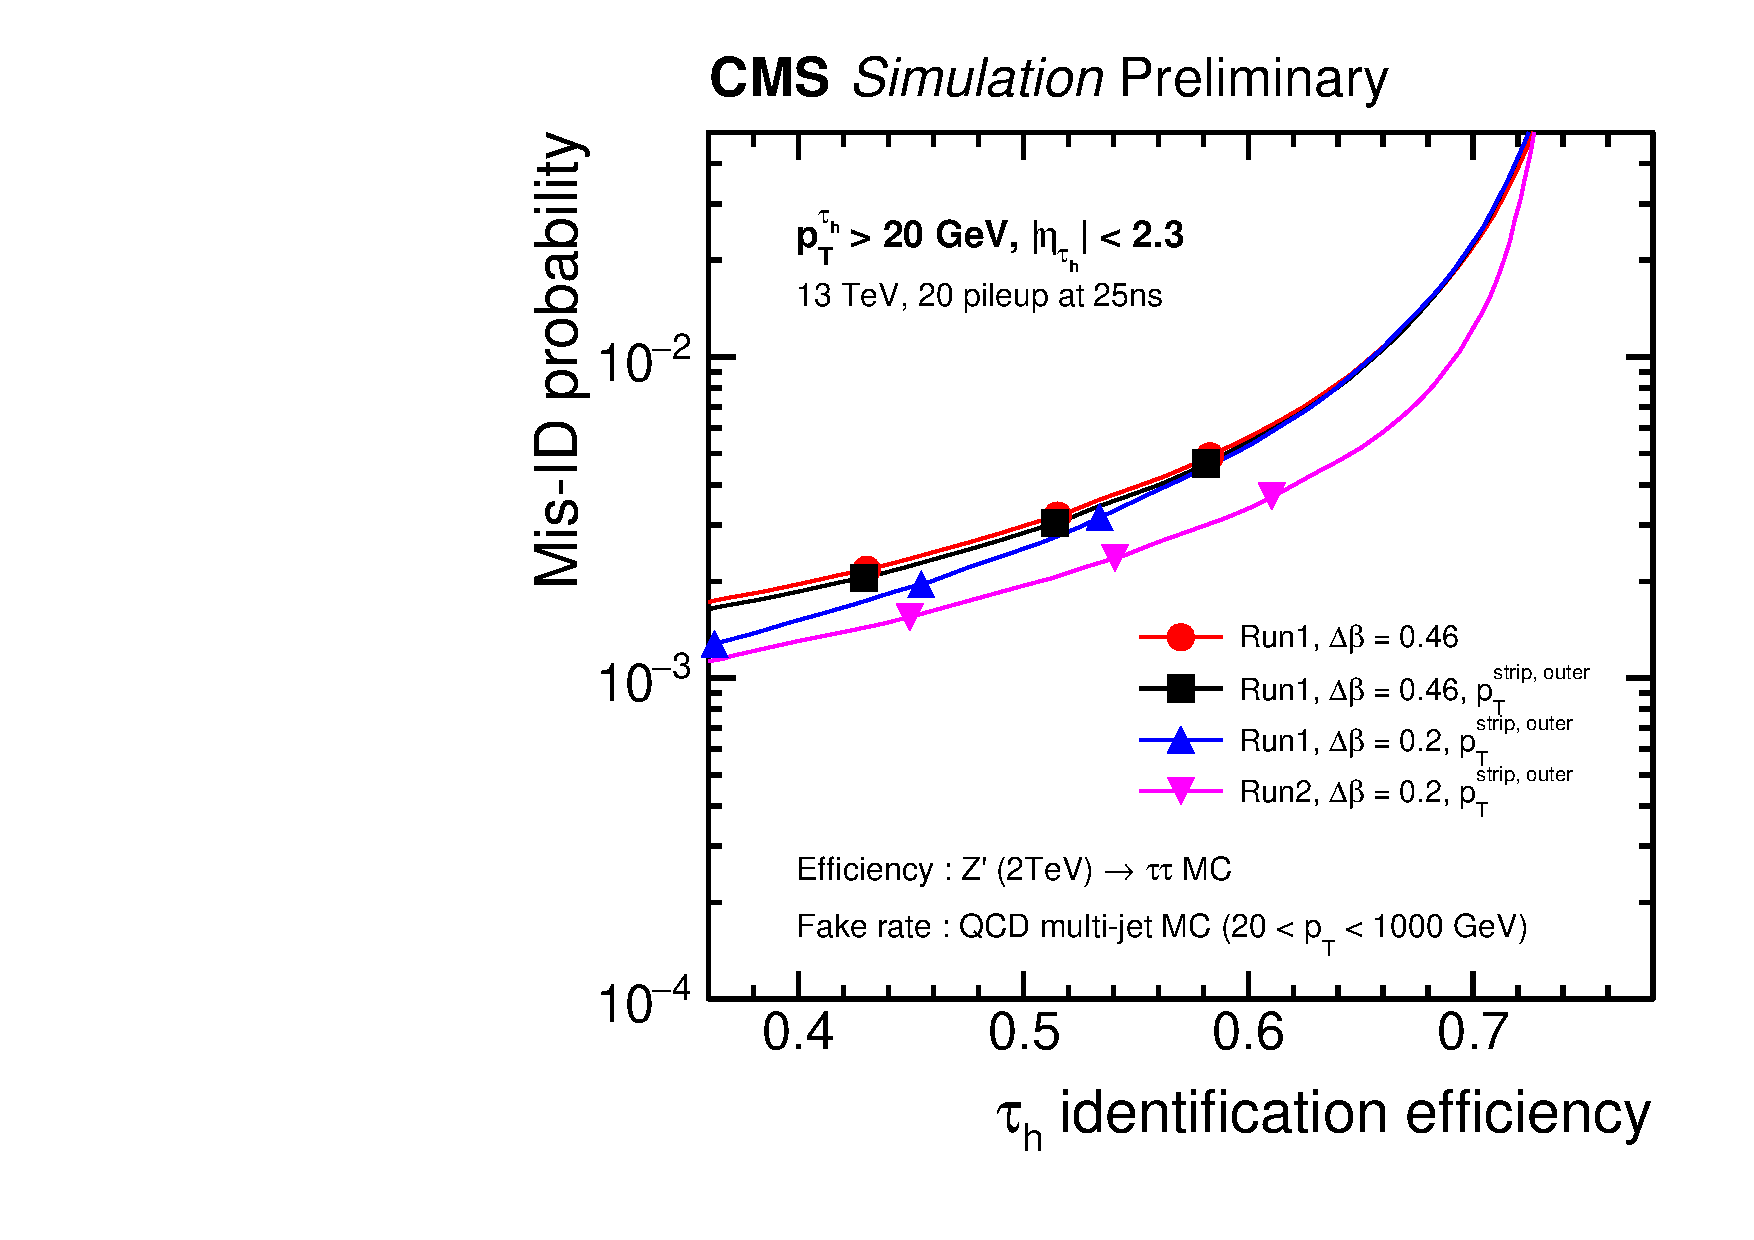
\includegraphics[width=0.4\textwidth]{figuras/Chapter3/IsoPerformanceZprime}
    \caption{Misidentification probability as a function of the \tauh~identification 
    efficiency, evaluated using $H \rightarrow \tau\tau$ (left) and \Zprimetotautau~(right), 
    and multijet MC samples. Four configurations of the reconstruction and 
    isolation method are compared (three of them for strip reconstruction using a 
    fixed  size, and the remaining one, for the dynamic-strip reconstruction). The three points 
    on each curve correspond to, from left to right, the tight, medium, and loose WPs. The
    misidentification probability is calculated relative to jets that pass minimal \tauh~reconstruction
    requirements. For the current version of the HPS algorithm (dynamic-strip reconstruction) the 
    tight isolation discriminator shows a better tau identification efficiency and a 
    lower misidentification rate. Taken from \cite{CMS-PAS-TAU-16-002}.
    }
    \label{fig:IsoSumPerformance}
  \end{center}
\end{figure} 

\noindent Additionally to the isolation-sum discriminator, in Run II, an \textit{MVA-based discriminator}
is applied for the tau identification. It has a better efficiency and a lower 
fake rate than the cutoff-based discriminator used in Run I. The MVA-based discriminator 
uses the following variables as input:
% Although they are less comprehensible, 
\begin{itemize}
 \item the \pt~and the $\eta$~direction of the \tauh~candidate,
  \item the transverse impact parameter $d_{0}$ of the \textit{leading} (highest-\pt) 
  track of the \tauh~candidate and its significance ($d_{0}/\sigma_{d_{0}}$),
 \item the isolation variable defined in equation \ref{eq:TauIso},
 \item the reconstructed decay mode,
 \item the multiplicity of photons an electrons, with \pt~$>$ 0.5 \GeV, that lie 
 within the signal and the isolation cones,
 \item the distance between the primary and secondary vertices and its significance, when
 the secondary vertex is identified.
\end{itemize}

\noindent The MVA-based discriminator is trained to distinguish the 
\tauh~candidate (signal) from QCD-jets (background). The MC samples used are: 
in the case of the signal, $Z/\gamma \rightarrow \tau\tau$, 
$H \rightarrow \tau\tau$, \Zprimetotautau, and $W^{\prime} \rightarrow 
\tau\bar{\nu_{\tau}}$; and in the case of the background, multijet, W+jets, and 
$t\bar{t}$. All the events were weighted such that the 
training of the MVA-discriminator was independent of the \pt~and 
$\eta$~distributions of the \tauh. Once the discriminator was trained, five working points were
defined according to the \tauh~identification efficiency. Figure \ref{fig:IsoPerformance} shows 
a comparison among the working points of the MVA-based and 
cutoff-based (Run I) discriminators, which were estimated 
with $H \rightarrow \tau\tau$ and \Zprimetotautau~MC samples for the 
signal, and QCD multijet MC samples for the background. 

\begin{figure}[ht]
  \begin{center}
    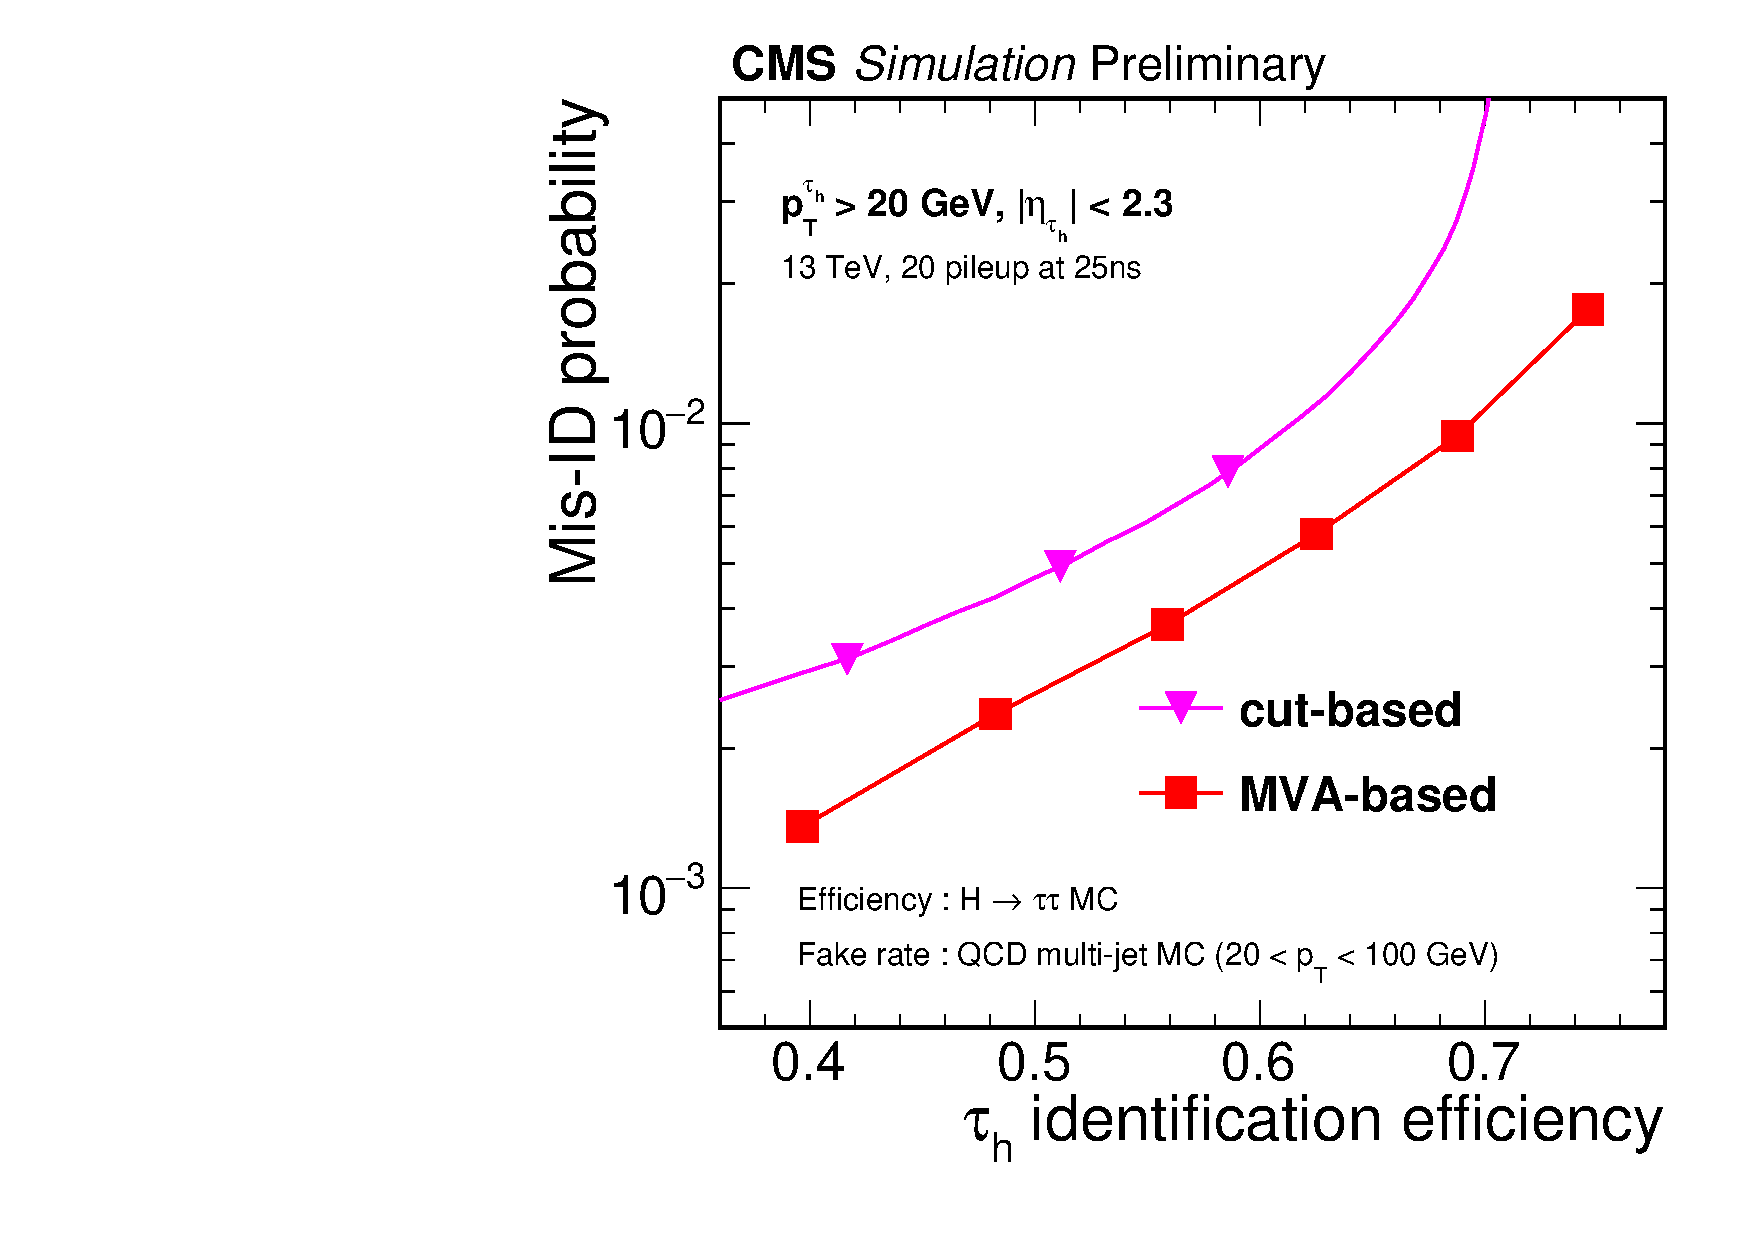
\includegraphics[width=0.4\textwidth]{figuras/Chapter3/MVAIsoPerformanceHiggs}
    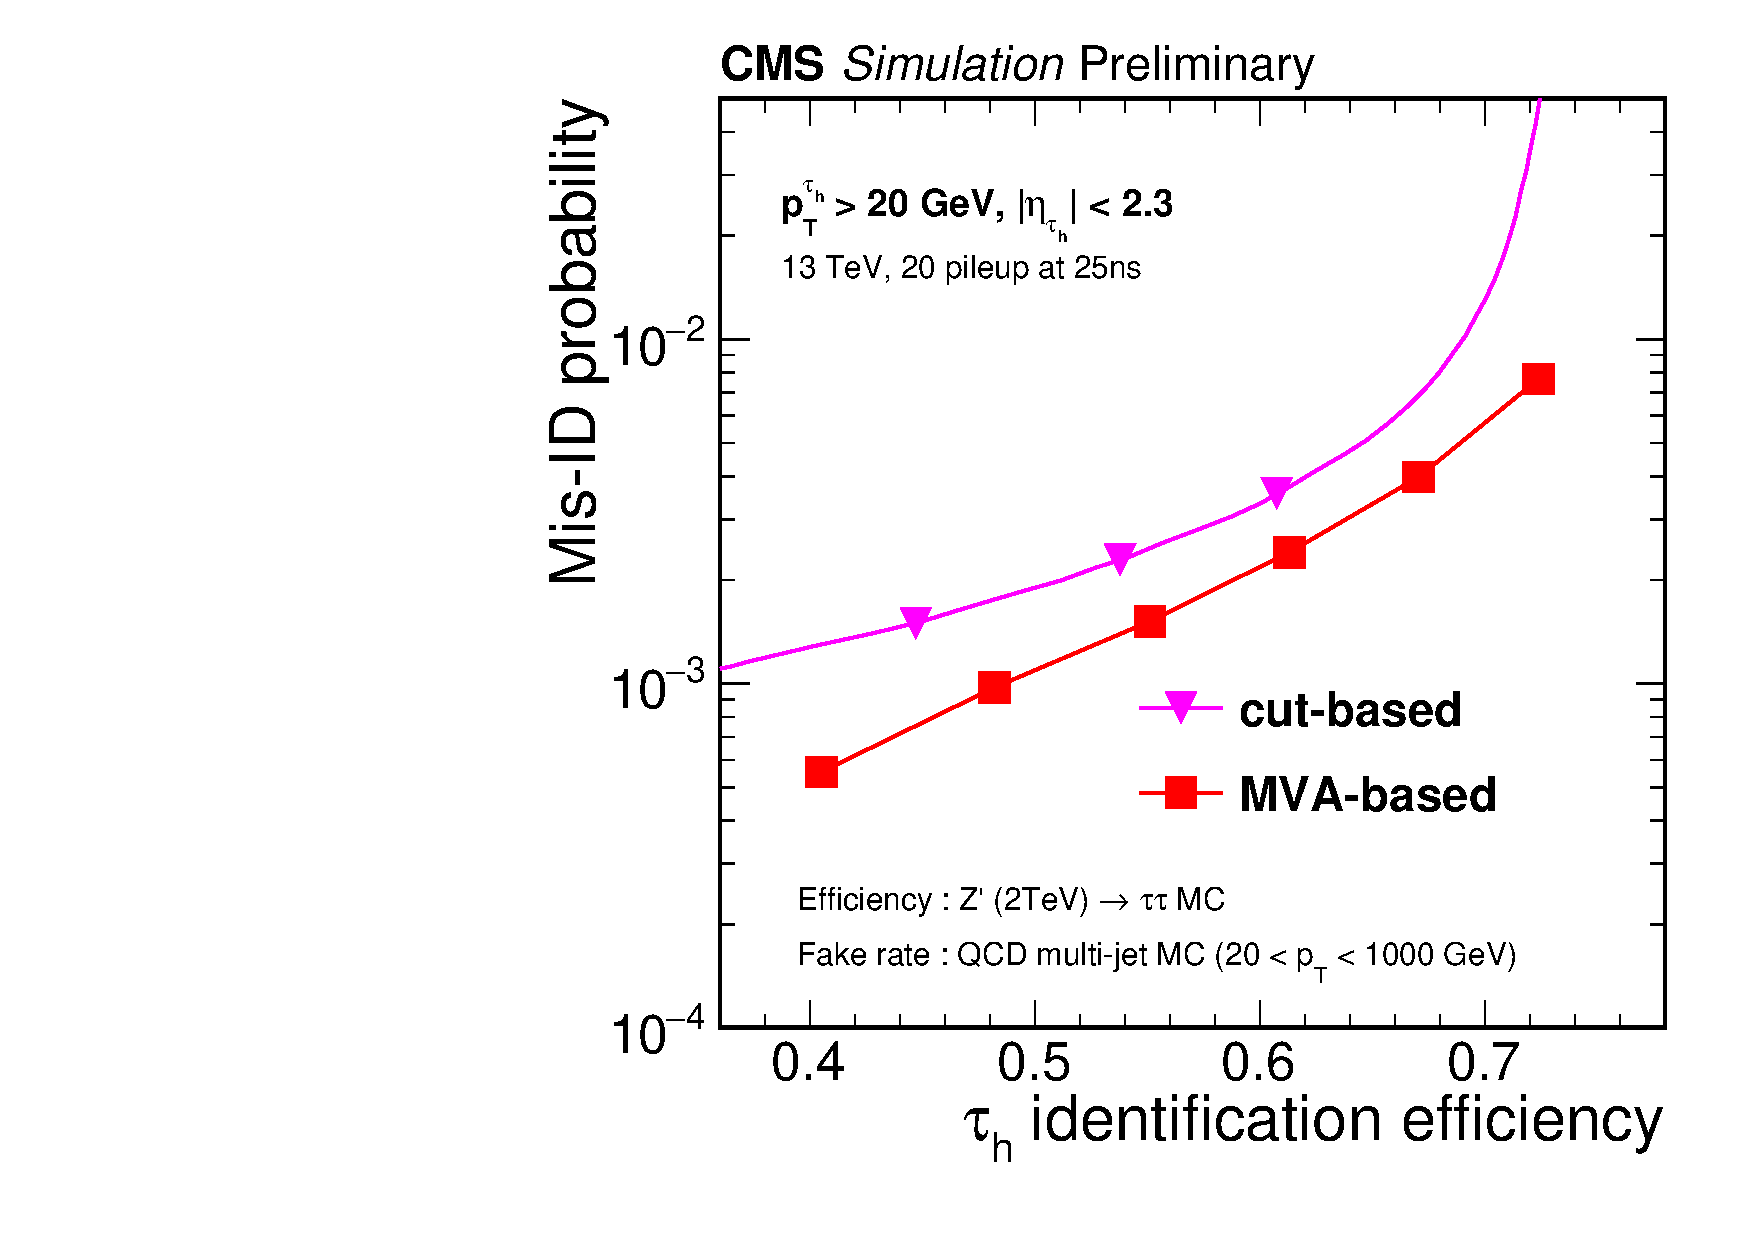
\includegraphics[width=0.4\textwidth]{figuras/Chapter3/MVAIsoPerformanceZprime}
    \caption{Misidentification probability as a function of \tauh~identification 
    efficiency, evaluated using $H \rightarrow \tau\tau$ and QCD MC samples (left), and \Zprime~(2 \TeV) 
    and QCD MC samples (right). The MVA-based discriminators are compared to 
    that of the isolation sum discriminators. The points correspond to working points 
    of the discriminators. The three working points of the isolation-sum discriminator 
    are Loose, Medium, and Tight working point. The six working points of the MVA-based 
    discriminators are Very Loose, Loose, Medium, Tight, Very Tight, and Very Very
    Tight working point, respectively. The misidentification probability is calculated with respect
    to jets, which pass minimal $\tau$~reconstruction requirements. Taken from \cite{CMS-PAS-TAU-16-002}.
    }
    \label{fig:IsoPerformance}
  \end{center}
\end{figure} 

\noindent Figure \ref{fig:TauEff} shows the expected identification 
efficiency and the misidentification rate, as a function of \pt, for each 
MVA-based working point. In this analysis, the MVA-based Tight 
discriminator WP is used in order to achieve a high purity in 
the di-$\tau$~selection, while keeping a considerable 
QCD-jet background rejection. For the current 
%since the dominant background comes from di-QCD jet events. For the current 
version of the HPS algorithm, the MVA-based tight discriminator 
has a $\tau$~identification efficiency of $\sim$60$\%$, and the 
QCD jet rejection rate is  $\sim$99.8$\%$. 

\begin{figure}[ht]
  \begin{center}
    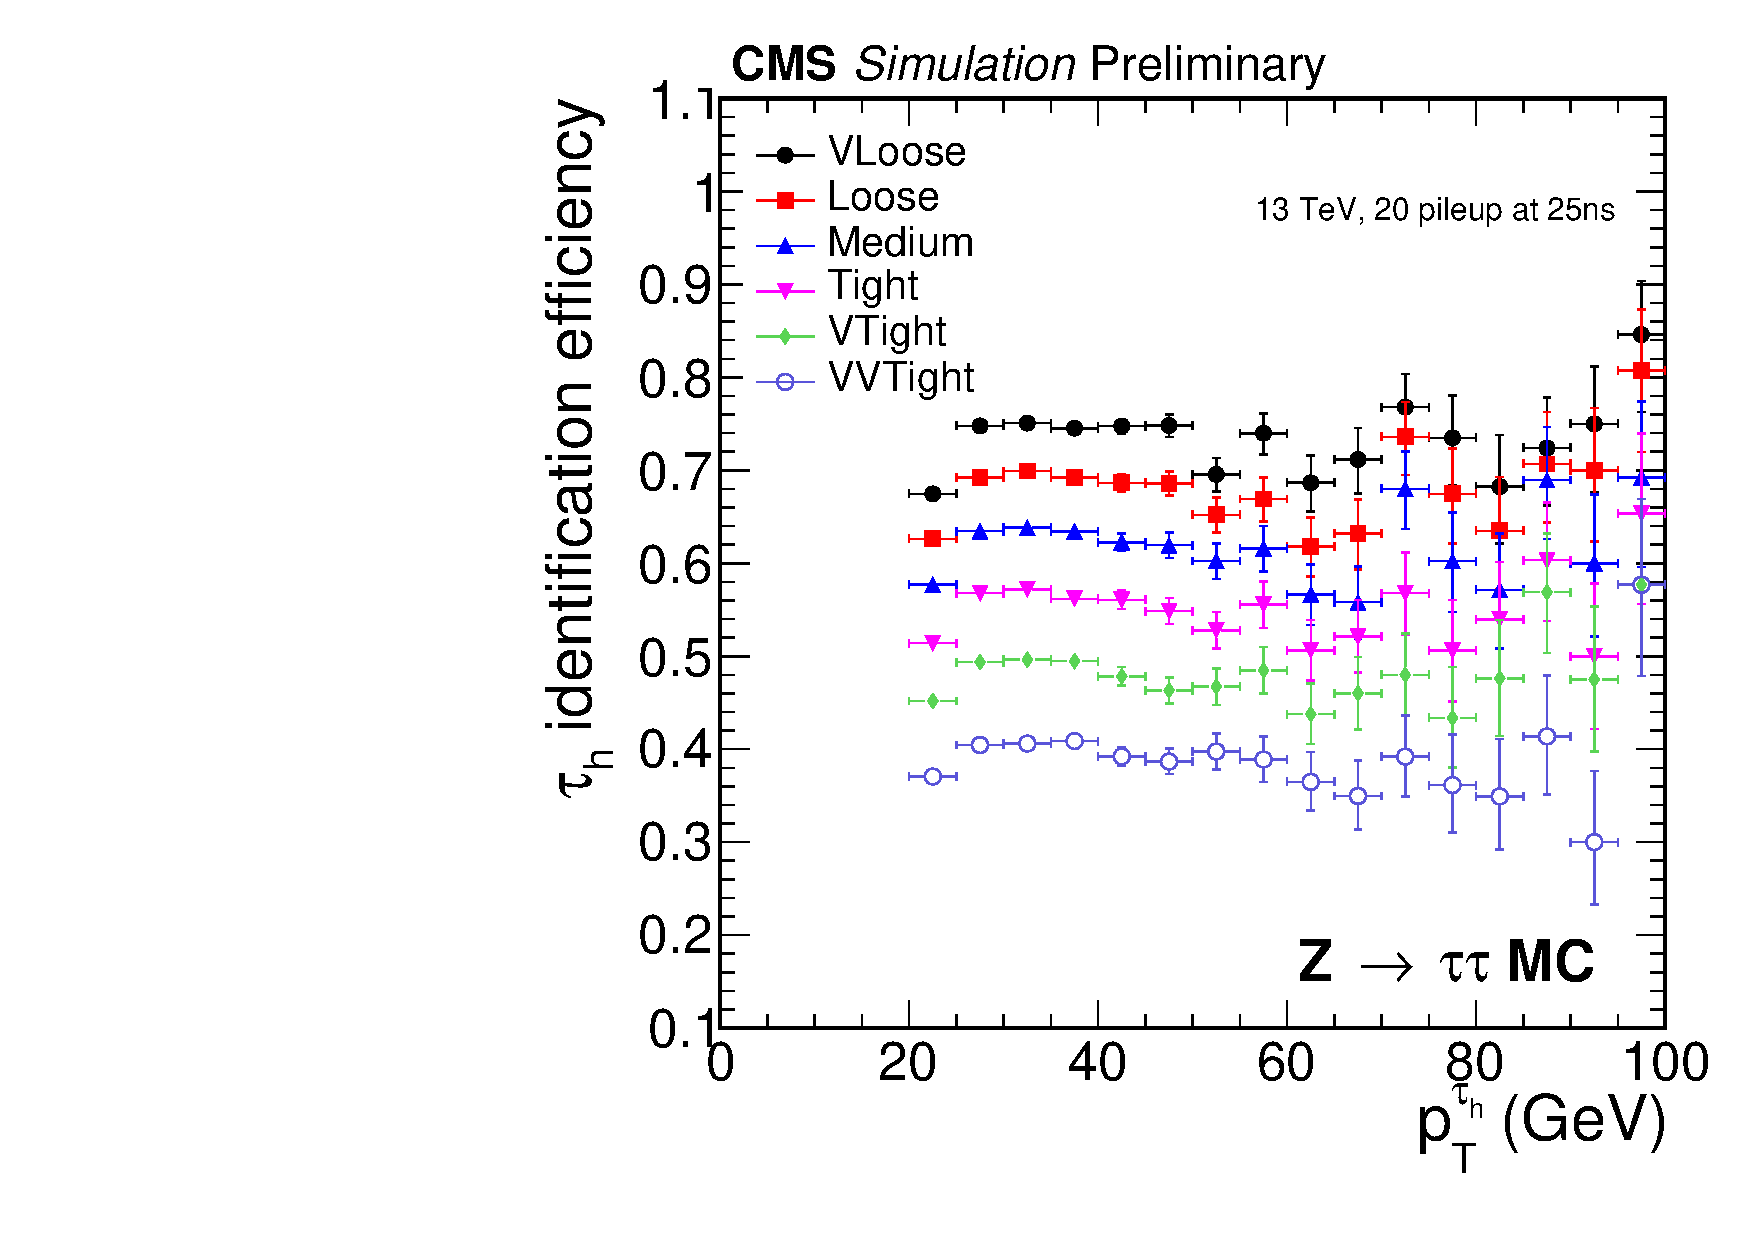
\includegraphics[width=0.4\textwidth]{figuras/Chapter3/TauEfficiency}
    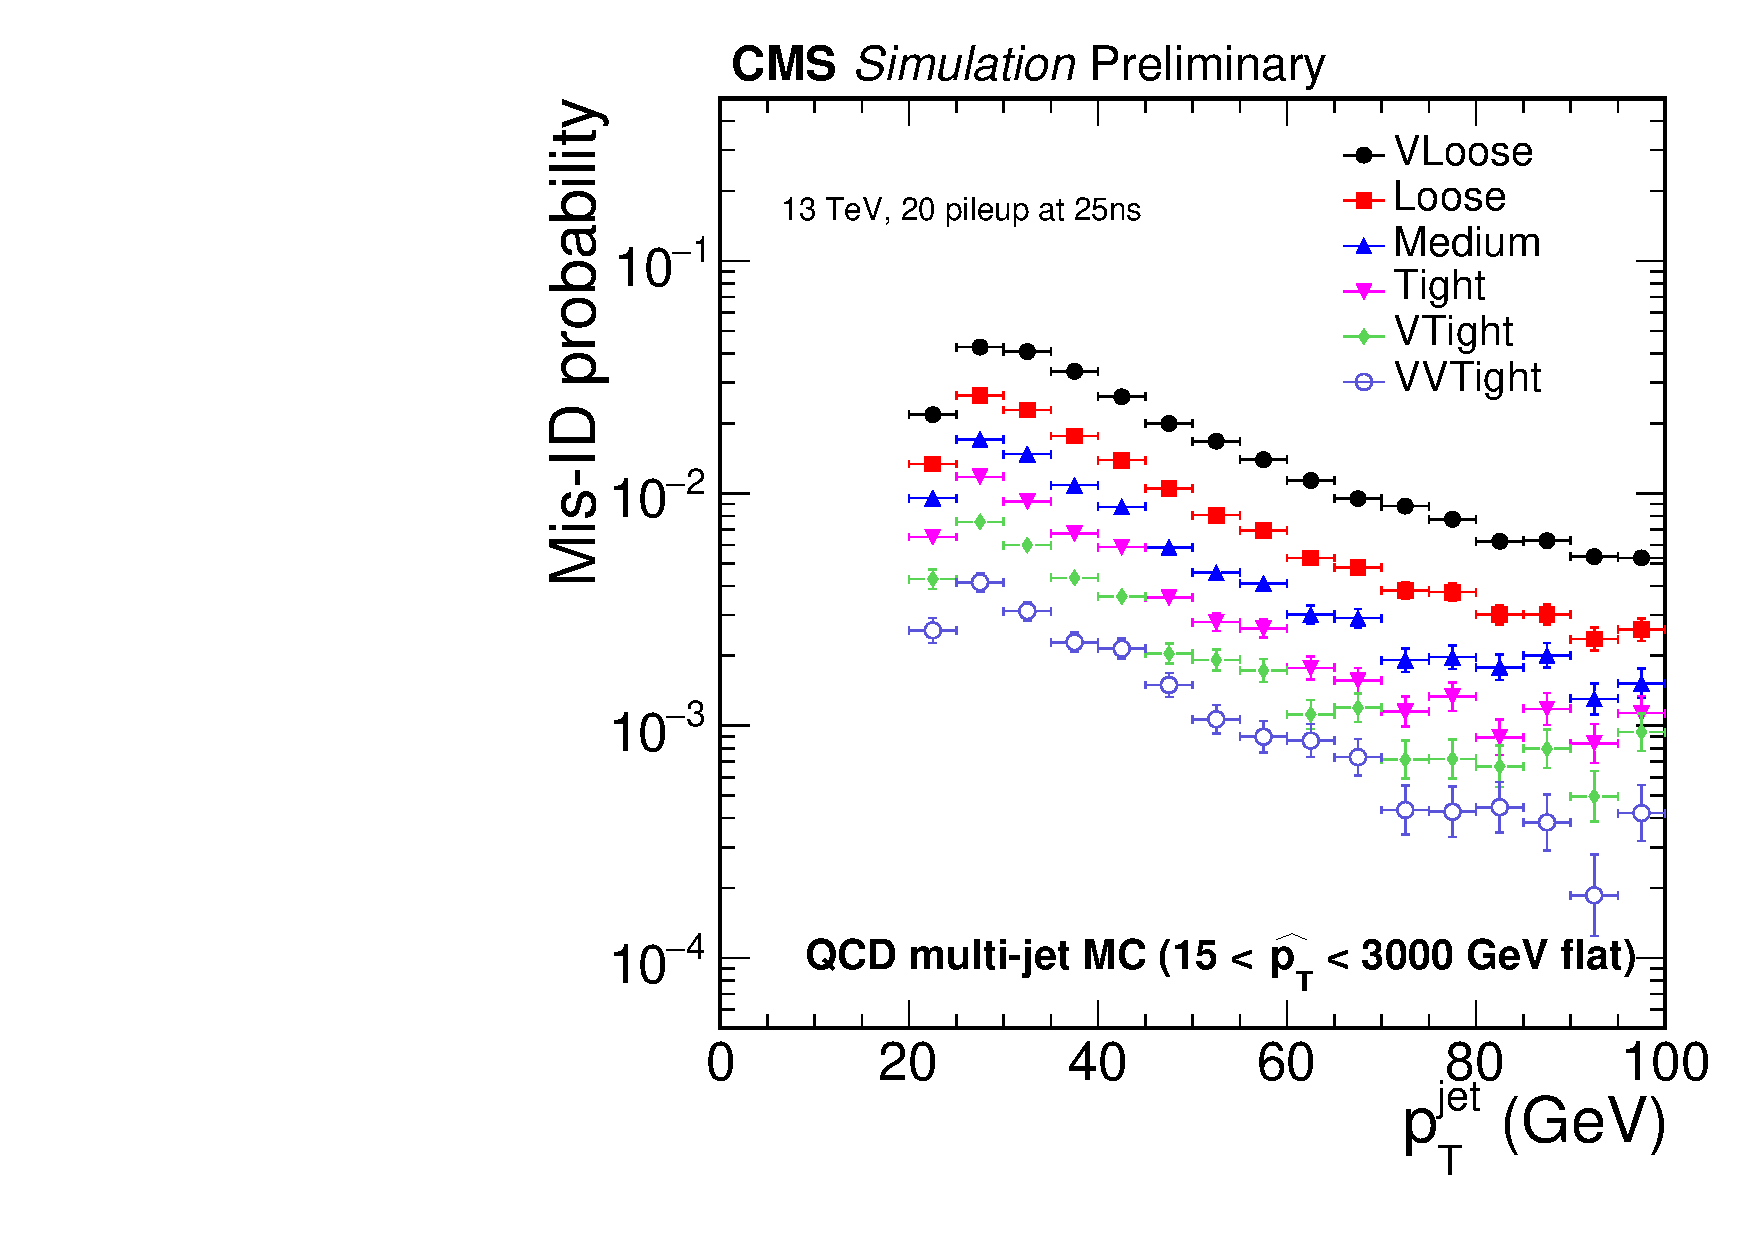
\includegraphics[width=0.4\textwidth]{figuras/Chapter3/TauMissID}
    \caption{
    Efficiency of the \tauh~identification estimated with simulated $Z/\gamma \rightarrow \tau\tau$ events (left)
    and the misidentification probability estimated with simulated QCD multi-jet events (right) for 
    the Very Loose, Loose, Medium, Tight, Very Tight, and Very Very Tight working points of the MVA 
    based \tauh-isolation algorithm. The efficiency is shown as a function of the \tauh~transverse 
    momentum while the misidentification probability is shown as a function of the jet transverse momentum. Taken from \cite{CMS-PAS-TAU-16-002}.
    }
    \label{fig:TauEff}
  \end{center}
\end{figure} 

\subsubsection{Tau Discrimination against electrons}
\label{subsubsec:DiscriminatorsAgainstElectron}

\noindent An electron signature has some probability to be misidentified as 
a $h^{\pm}$, or a $h^{\pm}$ \picero, decay modes of a tau. The probability 
is higher in the last case, since electrons emit bremsstrahlung that
can convert into photons in the tracker material, faking the \picero~signature. In 
consequence, a MVA-algorithm has been developed in order to discriminate 
electrons from taus, exploiting \tauh~features like the amount of 
Bremsstrahlung associated to the leading track and the low 
multiplicity of particles. The MVA-based against electrons discriminator 
uses the following variables as input:
\begin{itemize}
 \item the \pt~and the $\eta$~direction of the \tauh~candidate,
 \item the mass of the \tauh~candidate,
 \item the Electromagnetic energy fraction, $E_{ECAL}/(E_{ECAL}+E_{HCAL})$, of all 
 PF candidates associated to the \tauh,
 \item the ECAL and HCAL energies relative to the momentum of the leading charged-hadron 
 track ($E_{ECAL}/\textrm{p}_{\textrm{T}}^{\textrm{lead}}$ and $E_{HCAL}/\textrm{p}_{\textrm{T}}^{\textrm{lead}}$),
 \item the \pt-weighted root-mean-squared distances in the $\eta$ and the $\phi$ directions 
 ($\sqrt{\sum(\Delta \eta)^{2}\textrm{p}_{\textrm{T}}}$ and 
 $\sqrt{\sum(\Delta \phi)^{2}\textrm{p}_{\textrm{T}}}$) between the strips and the leading 
 charged-hadron track,
 \item the fraction of the tau energy carried by the photons ($\sum E_{\gamma} / E_{\tau}$),
 \item the ratio between the ECAL energy and the inner tracker momentum, $(E_{e}+\sum E_{\gamma})/p_{in}$,
 \item the Bremsstrahlung fraction $f_{brem}$ measured by the GSF (see Section \ref{sec:Electron}),
 \item the $\chi^{2}/N_{dof}$ of the GSF,
 \item the fraction $(N_{hits}^{\textrm{GSF}}-N_{hits}^{\textrm{KF}})/(N_{hits}^{\textrm{GSF}}+N_{hits}^{\textrm{KF}})$, where
 $N_{hits}^{\textrm{GSF}}$ and $N_{hits}^{\textrm{KF}}$ are the number of hits associated to the track by the GSF and the KF algorithms,
 respectively since they will show up any Bremsstrahlung emission in the Tracker System. 
\end{itemize}
 
\noindent The MVA-based against discriminator is trained with the MC samples: 
$Z/\gamma \rightarrow \tau\tau$, $H~\rightarrow \tau\tau$, \Zprimetotautau, and $W^{\prime}~
\rightarrow \tau\bar{\nu_{\tau}}$ for the signal, while
$Z/\gamma \rightarrow ee$, $H \rightarrow ee$, \Zprime~$\rightarrow ee$, and $W^{\prime}~
\rightarrow e\bar{\nu_{e}}$ for the background. Five WP are defined according to the 
tau-reconstruction efficiency. The efficiency and the misidentification rate are uniform over 
\pt~(see Figure \ref{fig:AgainstElectron}). In this 
analysis the Loose MVA-based against electron discriminator is used 
since it keeps a high tau reconstruction efficiency ($\sim$83$\%$) and a relative 
low fake rate ($10 ^{-2}$).

 \begin{figure}[ht]
   \begin{center}
     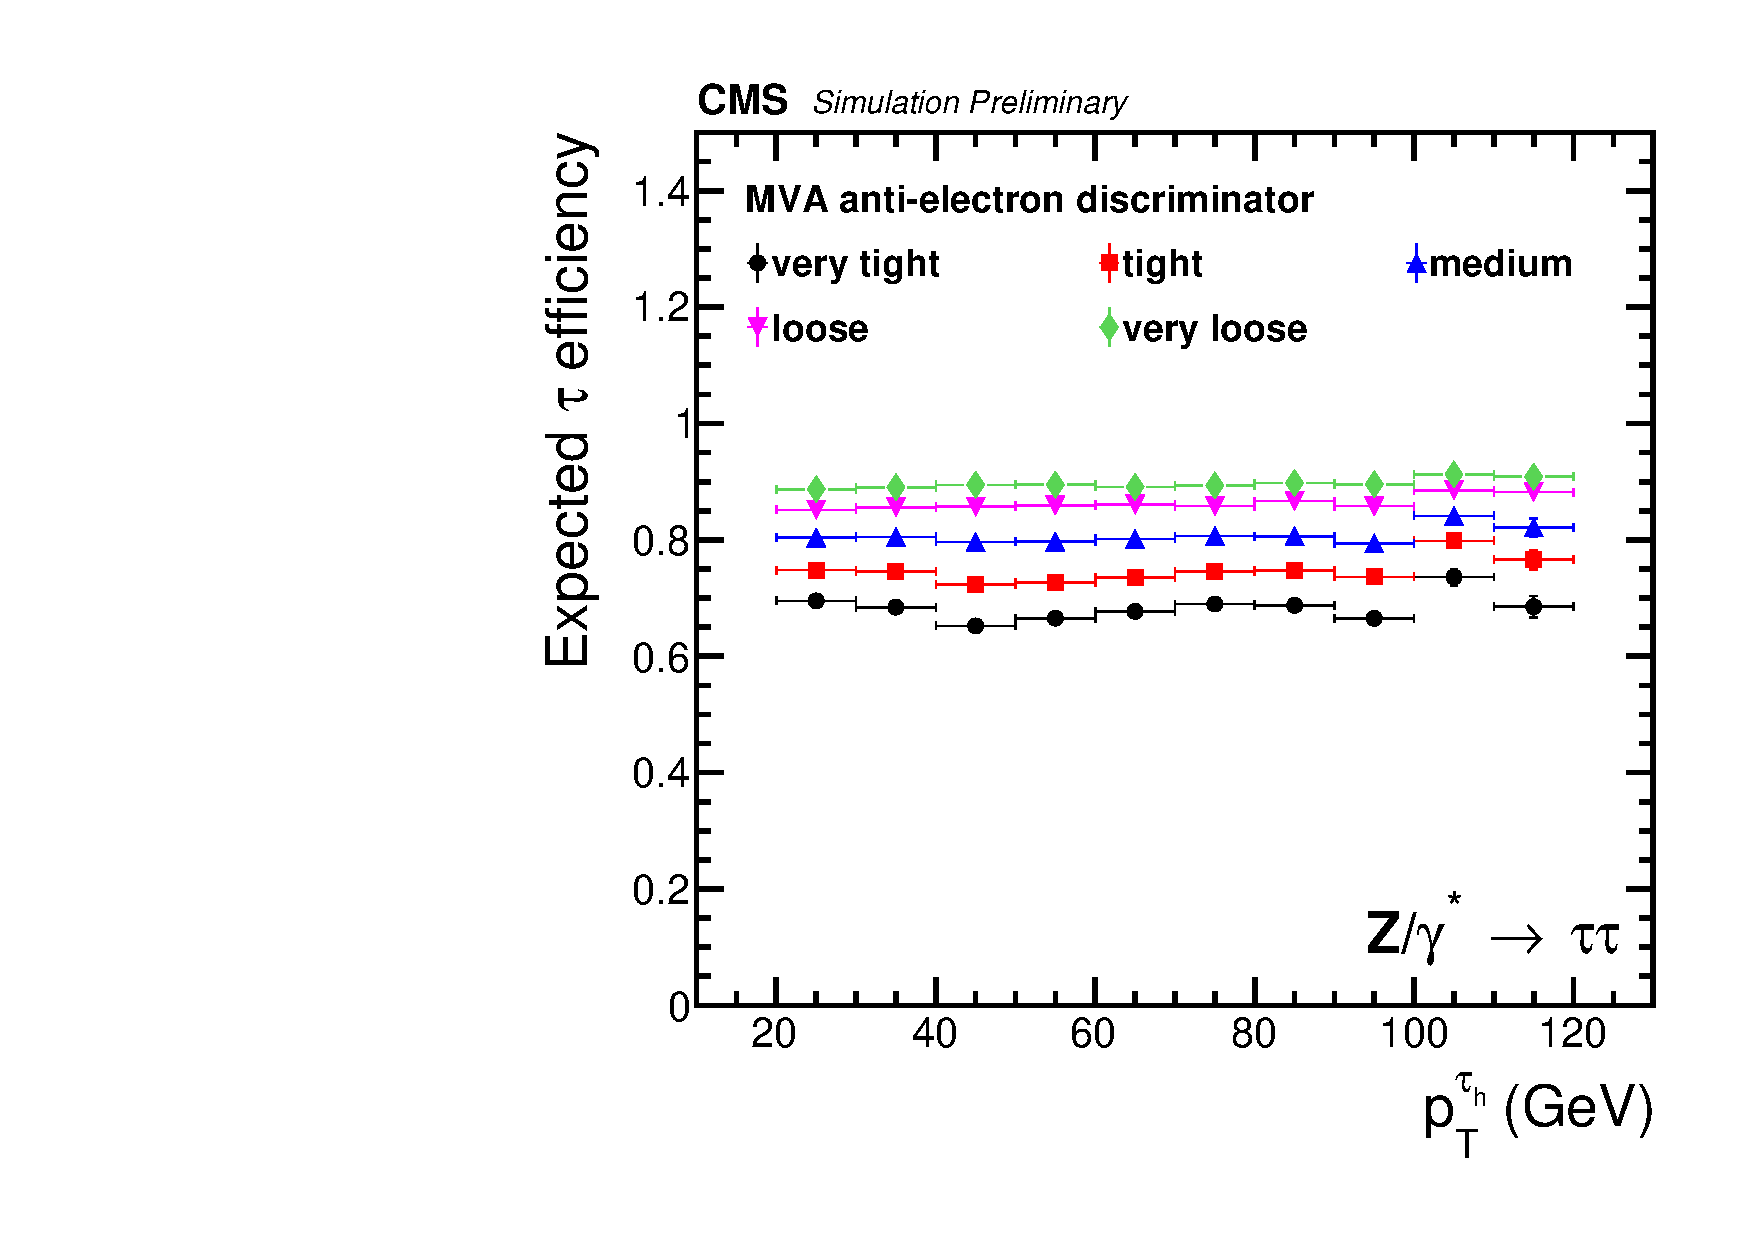
\includegraphics[width=0.4\textwidth]{figuras/Chapter3/TauEffAgainstElectrons}
     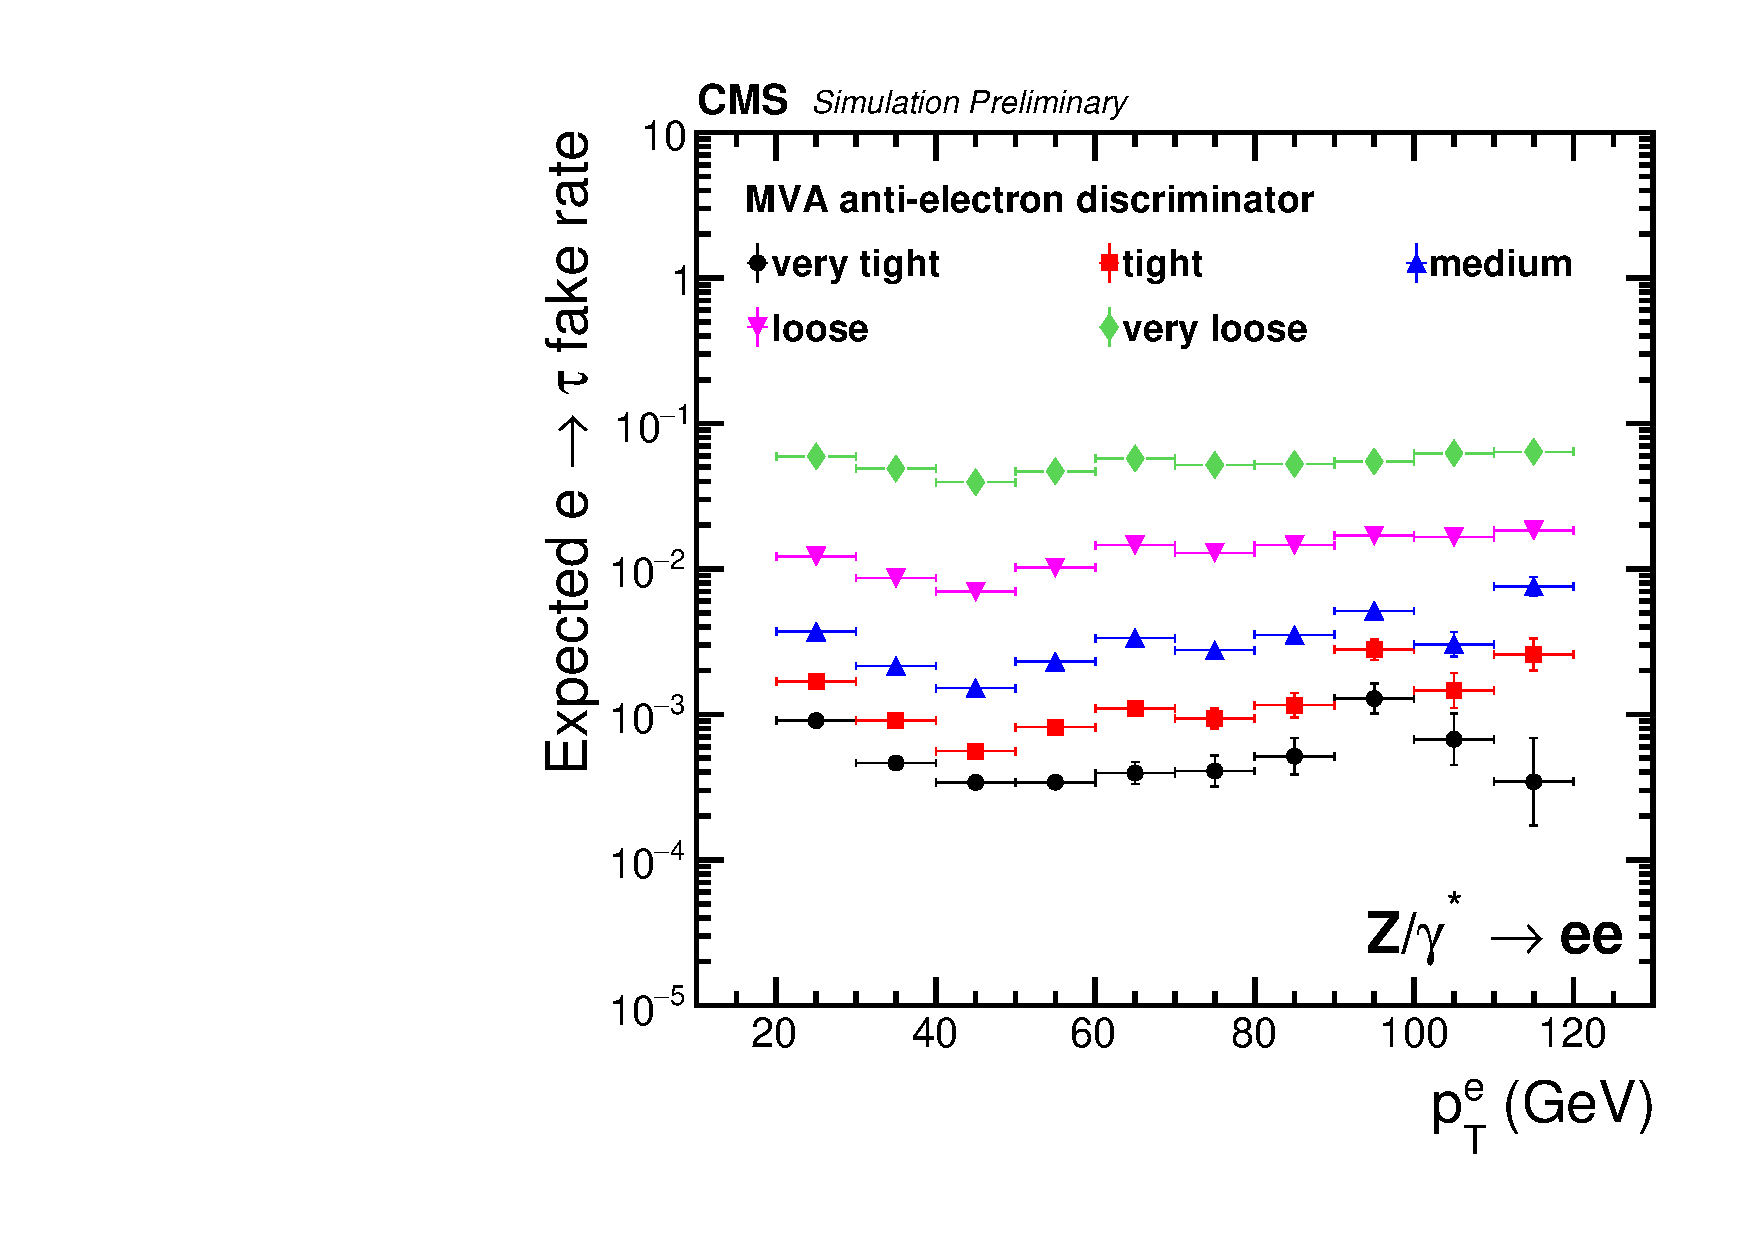
\includegraphics[width=0.4\textwidth]{figuras/Chapter3/FakeRateAgainstElectrons}
     \caption{
     Efficiency of the \tauh~identification estimated with simulated $Z/\gamma^{*}\rightarrow\tau\tau$ (left) 
      and the $e \rightarrow \tau_{h}$ misidentification probability estimated with simulated $Z/\gamma^{*}\rightarrow ee$ 
    events (right) for the Very Loose, Loose, Medium, Tight and Very Tight working points of the MVA based 
    anti-$e$ discrimination algorithm. The efficiency is shown as a function of the \tauh~transverse momentum 
    while the misidentification probability is shown as a function of the $e$ transverse momentum. Both 
    efficiency and misidentification probability are calculated for \tauh~candidates with a reconstructed 
    decay mode and passing the Loose working point of the isolation sum-discriminator. Taken from \cite{CMS-PAS-TAU-16-002}.
     }
     \label{fig:AgainstElectron}
   \end{center}
 \end{figure} 


\subsubsection{Tau Discrimination against muons}
\label{subsubsec:DiscriminatorsAgainstMuon}

\noindent A muon signature can fake the one produced by a $h^{\pm}$ decay mode 
of a \tauh; due to this, discriminants have been developed in order to 
distinguish between them. The cutoff-based discriminator
is used since it has a similar efficiency than the MVA-based one. Two 
working points have been defined:

\begin{itemize}
 \item \textbf{Loose}: A \tauh~candidate fails this discriminant when at least two track segments are found 
 in the Muon Chambers within a cone of size $\Delta R < 0.3$ and centered in the \tauh~direction, or when 
 the sum of the ECAL and HCAL energy deposits are less than 20$\%$ of the momentum of the leading track
 of the \tauh~candidate.
 \item \textbf{Tight}: A \tauh~candidate passes this discriminant when it has passed the Loose WP and no hits are found in 
 the CSCs, DTs and RPCs located in the two outermost Muon stations, within a cone of size $\Delta R < 0.3$ and 
 centered in the \tauh~direction.
\end{itemize}

\noindent The tau identification efficiency for both WPs is more that 99$\%$ and
the misidentification probability is 3.5 $\times 10^{-3}$ and 1.4 $\times 10^{-3}$
for the loose and tight WP, respectively. In this analysis, the tight working point is used.\\


\noindent In summary, in this analysis the hadronic taus are reconstructed using the HPS algorithm,
requiring 1or3-prongs with the \textit{newDMF} discriminator. The signal cone has 
a radius of $R_{sig}=3.0 / \textrm{p}_{\textrm{T}} (\textrm{GeV})$ and it is centered in 
the direction of the tau momentum. Since jets are used as input for 
the HPS algorithm, its reconstruction is also crucial in this analysis. Jets are reconstructed 
using anti-kT algorithm (loose WP), with the distance parameter $\Delta R(\phi,\eta) =$ 0.4.
Jets are required to have \pt~$>$ 30 \GeV~ and $|\eta| <$ 2.4. In order to identify
the hadronic taus from QCD-jets, the \textit{tight} WP of MVA-based isolation discriminator was 
 used, reaching a $\sim$60$\%$  of $\tau$~identification efficiency and 
 a $\sim$99.8$\%$ of rejection rate against QCD jets. The isolation cone has a 
size of $\Delta R =$ 0.5 and it is centered in the \tauh~direction. Since
b-jets can be misidentified as a hadronic taus, their identification are also 
important for the \Zprimetotauh~search. The b-Jets are reconstructed using 
the \textit{loose} working point of the CSVv2 algorithm, which provides an efficiency of
83$\%$. In order to discriminate taus from electrons, the \textit{loose} MVA-based discriminator 
was used, achieving a tau reconstruction efficiency of $\sim$83$\%$ and keeping a misidentification
 rate of the order of $10 ^{-2}$. The electrons are reconstructed using the 90$\%$ efficiency 
 working point of the MVA-based electron ID algorithm, with the isolation requirement of $\Delta R <$ 0.4.
 In order to discriminate taus from muons, the \textit{tight} WP of cutoff-based discriminator was
 required, which reaches a 99$\%$ of tau reconstruction efficiency and a 1.4 $\times 10^{-3}$ 
 of misidentification rate. For the muon reconstruction, ``global muons'' with an 
 isolation cone of $\Delta R <$ 0.4 are required. The \METv~is reconstructed
 with the PF algorithm, where the “type-I” correction is applied. 

%The jet p T resolutions are determined with both dijet and photon+jet events, as discussed in
%section 8. The reference resolutions obtained from simulation are parameterized as a function of
%particle-level jet p T, ptcl (defined in section 2) and average number μ of pileup interactions in bins
%of jet η. Corrections for differences between data and MC simulation are applied as η-binned scale
%factors

%PF jet momentum and spatial resolutions are greatly improved with respect to calorimeter jets, as
%the use of the tracking detectors and high granularity of the ECAL improves the energy resolution
%through the independent measurements of charged hadrons and photons inside a jet, which together
%2.1constitute ≈85% of the average jet energy. In reconstructing the PF candidate four-momentum,
%photons are assumed massless and charged hadrons are assigned the charged pion mass.
